\newif\ifws
%\wstrue
\ifws


%  LaTeX support: latex@mdpi.com
%  For support, please attach all files needed for compiling as well as the log file, and specify your operating system, LaTeX version, and LaTeX editor.

%=================================================================
\documentclass[entropy,article,submit,pdftex,oneauthor]{Definitions/mdpi}
%\documentclass[entropy,article,submit,pdftex,moreauthors]{Definitions/mdpi}
%\documentclass[preprints,article,submit,pdftex,moreauthors]{Definitions/mdpi}
% For posting an early version of this manuscript as a preprint, you may use "preprints" as the journal. Changing "submit" to "accept" before posting will remove line numbers.

% Below journals will use APA reference format:
% admsci, behavsci, businesses, econometrics, economies, education, ejihpe, games, humans, ijfs, journalmedia, jrfm, languages, psycholint, publications, tourismhosp, youth

% Below journals will use Chicago reference format:
% arts, genealogy, histories, humanities, jintelligence, laws, literature, religions, risks, socsci

%--------------------
% Class Options:
%--------------------
%----------
% journal
%----------
% Choose between the following MDPI journals:
% accountaudit, acoustics, actuators, addictions, adhesives, admsci, adolescents, aerobiology, aerospace, agriculture, agriengineering, agrochemicals, agronomy, ai, air, algorithms, allergies, alloys, amh, analytica, analytics, anatomia, anesthres, animals, antibiotics, antibodies, antioxidants, applbiosci, appliedchem, appliedmath, appliedphys, applmech, applmicrobiol, applnano, applsci, aquacj, architecture, arm, arthropoda, arts, asc, asi, astronomy, atmosphere, atoms, audiolres, automation, axioms, bacteria, batteries, bdcc, behavsci, beverages, biochem, bioengineering, biologics, biology, biomass, biomechanics, biomed, biomedicines, biomedinformatics, biomimetics, biomolecules, biophysica, biosensors, biosphere, biotech, birds, blockchains, bloods, blsf, brainsci, breath, buildings, businesses, cancers, carbon, cardiogenetics, catalysts, cells, ceramics, challenges, chemengineering, chemistry, chemosensors, chemproc, children, chips, cimb, civileng, cleantechnol, climate, clinbioenerg, clinpract, clockssleep, cmd, cmtr, coasts, coatings, colloids, colorants, commodities, complications, compounds, computation, computers, condensedmatter, conservation, constrmater, cosmetics, covid, crops, cryo, cryptography, crystals, csmf, ctn, curroncol, cyber, dairy, data, ddc, dentistry, dermato, dermatopathology, designs, devices, diabetology, diagnostics, dietetics, digital, disabilities, diseases, diversity, dna, drones, dynamics, earth, ebj, ecm, ecologies, econometrics, economies, education, eesp, ejihpe, electricity, electrochem, electronicmat, electronics, encyclopedia, endocrines, energies, eng, engproc, ent, entomology, entropy, environments, epidemiologia, epigenomes, esa, est, famsci, fermentation, fibers, fintech, fire, fishes, fluids, foods, forecasting, forensicsci, forests, fossstud, foundations, fractalfract, fuels, future, futureinternet, futureparasites, futurepharmacol, futurephys, futuretransp, galaxies, games, gases, gastroent, gastrointestdisord, gastronomy, gels, genealogy, genes, geographies, geohazards, geomatics, geometry, geosciences, geotechnics, geriatrics, glacies, grasses, greenhealth, gucdd, hardware, hazardousmatters, healthcare, hearts, hemato, hematolrep, heritage, higheredu, highthroughput, histories, horticulturae, hospitals, humanities, humans, hydrobiology, hydrogen, hydrology, hygiene, idr, iic, ijerph, ijfs, ijgi, ijmd, ijms, ijns, ijpb, ijt, ijtm, ijtpp, ime, immuno, informatics, information, infrastructures, inorganics, insects, instruments, inventions, iot, j, jal, jcdd, jcm, jcp, jcs, jcto, jdad, jdb, jeta, jfb, jfmk, jimaging, jintelligence, jlpea, jmahp, jmmp, jmms, jmp, jmse, jne, jnt, jof, joitmc, joma, jop, jor, journalmedia, jox, jpbi, jpm, jrfm, jsan, jtaer, jvd, jzbg, kidney, kidneydial, kinasesphosphatases, knowledge, labmed, laboratories, land, languages, laws, life, lights, limnolrev, lipidology, liquids, literature, livers, logics, logistics, lubricants, lymphatics, machines, macromol, magnetism, magnetochemistry, make, marinedrugs, materials, materproc, mathematics, mca, measurements, medicina, medicines, medsci, membranes, merits, metabolites, metals, meteorology, methane, metrics, metrology, micro, microarrays, microbiolres, microelectronics, micromachines, microorganisms, microplastics, microwave, minerals, mining, mmphys, modelling, molbank, molecules, mps, msf, mti, multimedia, muscles, nanoenergyadv, nanomanufacturing, nanomaterials, ncrna, ndt, network, neuroglia, neurolint, neurosci, nitrogen, notspecified, nri, nursrep, nutraceuticals, nutrients, obesities, oceans, ohbm, onco, oncopathology, optics, oral, organics, organoids, osteology, oxygen, parasites, parasitologia, particles, pathogens, pathophysiology, pediatrrep, pets, pharmaceuticals, pharmaceutics, pharmacoepidemiology, pharmacy, philosophies, photochem, photonics, phycology, physchem, physics, physiologia, plants, plasma, platforms, pollutants, polymers, polysaccharides, populations, poultry, powders, preprints, proceedings, processes, prosthesis, proteomes, psf, psych, psychiatryint, psychoactives, psycholint, publications, purification, quantumrep, quaternary, qubs, radiation, reactions, realestate, receptors, recycling, regeneration, religions, remotesensing, reports, reprodmed, resources, rheumato, risks, robotics, rsee, ruminants, safety, sci, scipharm, sclerosis, seeds, sensors, separations, sexes, signals, sinusitis, siuj, skins, smartcities, sna, societies, socsci, software, soilsystems, solar, solids, spectroscj, sports, standards, stats, std, stresses, surfaces, surgeries, suschem, sustainability, symmetry, synbio, systems, tae, targets, taxonomy, technologies, telecom, test, textiles, thalassrep, therapeutics, thermo, timespace, tomography, tourismhosp, toxics, toxins, transplantology, transportation, traumacare, traumas, tropicalmed, universe, urbansci, uro, vaccines, vehicles, venereology, vetsci, vibration, virtualworlds, viruses, vision, waste, water, wem, wevj, wild, wind, women, world, youth, zoonoticdis

%---------
% article
%---------
% The default type of manuscript is "article", but can be replaced by:
% abstract, addendum, article, benchmark, book, bookreview, briefcommunication, briefreport, casereport, changes, clinicopathologicalchallenge, comment, commentary, communication, conceptpaper, conferenceproceedings, correction, conferencereport, creative, datadescriptor, discussion, entry, expressionofconcern, extendedabstract, editorial, essay, erratum, fieldguide, hypothesis, interestingimages, letter, meetingreport, monograph, newbookreceived, obituary, opinion, proceedingpaper, projectreport, reply, retraction, review, perspective, protocol, shortnote, studyprotocol, supfile, systematicreview, technicalnote, viewpoint, guidelines, registeredreport, tutorial,  giantsinurology, urologyaroundtheworld
% supfile = supplementary materials

%----------
% submit
%----------
% The class option "submit" will be changed to "accept" by the Editorial Office when the paper is accepted. This will only make changes to the frontpage (e.g., the logo of the journal will get visible), the headings, and the copyright information. Also, line numbering will be removed. Journal info and pagination for accepted papers will also be assigned by the Editorial Office.

%------------------
% moreauthors
%------------------
% If there is only one author the class option oneauthor should be used. Otherwise use the class option moreauthors.

%---------
% pdftex
%---------
% The option pdftex is for use with pdfLaTeX. Remove "pdftex" for (1) compiling with LaTeX & dvi2pdf (if eps figures are used) or for (2) compiling with XeLaTeX.

%=================================================================
% MDPI internal commands - do not modify
\firstpage{1}
\makeatletter
\setcounter{page}{\@firstpage}
\makeatother
\pubvolume{1}
\issuenum{1}
\articlenumber{0}
\pubyear{2025}
\copyrightyear{2025}
%\externaleditor{Firstname Lastname} % More than 1 editor, please add `` and '' before the last editor name
\datereceived{ }
\daterevised{ } % Comment out if no revised date
\dateaccepted{ }
\datepublished{ }
%\datecorrected{} % For corrected papers: "Corrected: XXX" date in the original paper.
%\dateretracted{} % For retracted papers: "Retracted: XXX" date in the original paper.
\hreflink{https://doi.org/} % If needed use \linebreak
%\doinum{}
%\pdfoutput=1 % Uncommented for upload to arXiv.org
%\CorrStatement{yes}  % For updates
%\longauthorlist{yes} % For many authors that exceed the left citation part

%=================================================================
% Add packages and commands here. The following packages are loaded in our class file: fontenc, inputenc, calc, indentfirst, fancyhdr, graphicx, epstopdf, lastpage, ifthen, float, amsmath, amssymb, lineno, setspace, enumitem, mathpazo, booktabs, titlesec, etoolbox, tabto, xcolor, colortbl, soul, multirow, microtype, tikz, totcount, changepage, attrib, upgreek, array, tabularx, pbox, ragged2e, tocloft, marginnote, marginfix, enotez, amsthm, natbib, hyperref, cleveref, scrextend, url, geometry, newfloat, caption, draftwatermark, seqsplit
% cleveref: load \crefname definitions after \begin{document}

%=================================================================
% Please use the following mathematics environments: Theorem, Lemma, Corollary, Proposition, Characterization, Property, Problem, Example, ExamplesandDefinitions, Hypothesis, Remark, Definition, Notation, Assumption
%% For proofs, please use the proof environment (the amsthm package is loaded by the MDPI class).

%=================================================================
% Full title of the paper (Capitalized)
\Title{Chromatic Quantum Contextuality}

% MDPI internal command: Title for citation in the left column
\TitleCitation{Chromatic Quantum Contextuality}

% Author Orchid ID: enter ID or remove command
\newcommand{\orcidauthorA}{0000-0001-6554-2802} % Add \orcidA{} behind the author's name
%\newcommand{\orcidauthorB}{0000-0000-0000-000X} % Add \orcidB{} behind the author's name

% Authors, for the paper (add full first names)
\Author{Karl Svozil $^{1,\dagger,\ddagger}$\orcidA{}}

%\longauthorlist{yes}

% MDPI internal command: Authors, for metadata in PDF
\AuthorNames{Karl Svozil}

% MDPI internal command: Authors, for citation in the left column, only choose below one of them according to the journal style
% If this is a Chicago style journal
% (arts, genealogy, histories, humanities, jintelligence, laws, literature, religions, risks, socsci):
% Lastname, Firstname, Firstname Lastname, and Firstname Lastname.

% If this is a APA style journal
% (admsci, behavsci, businesses, econometrics, economies, education, ejihpe, games, humans, ijfs, journalmedia, jrfm, languages, psycholint, publications, tourismhosp, youth):
% Lastname, F., Lastname, F., \& Lastname, F.

% If this is a ACS style journal (Except for the above Chicago and APA journals, all others are in the ACS format):
% Lastname, F.; Lastname, F.; Lastname, F.
\isAPAStyle{%
       \AuthorCitation{Svozil, K.}
         }{%
        \isChicagoStyle{%
        \AuthorCitation{Svozil,Karl}
        }{
        \AuthorCitation{Svozil, K.}
        }
}

% Affiliations / Addresses (Add [1] after \address if there is only one affiliation.)
\address{%
$^{1}$ \quad Institute for Theoretical Physics,
TU Wien,
Wiedner Hauptstrasse 8-10/136,
1040 Vienna,  Austria; karl.svozil@tuwien.ac.at}

% Contact information of the corresponding author
\corres{Correspondence: karl.svozil@tuwien.ac.at}

% Current address and/or shared authorship
%\firstnote{Current address: Affiliation.}  % Current address should not be the same as any items in the Affiliation section.
%\secondnote{These authors contributed equally to this work.}
% The commands \thirdnote{} till \eighthnote{} are available for further notes

%\simplesumm{} % Simple summary

%\conference{} % An extended version of a conference paper

% Abstract (Do not insert blank lines, i.e. \\)
\abstract{
Chromatic quantum contextuality is a criterion of quantum nonclassicality based on (hyper)graph coloring constraints. If a quantum hypergraph requires more colors than the number of outcomes per maximal observable (context), it lacks a classical realization with $n$-uniform outcomes per context. Consequently, it cannot represent a ``completable'' non-contextual set of coexisting $n$-ary outcomes per maximal observable. This result serves as a chromatic analogue of the Kochen-Specker theorem. We present an explicit example of a four-colorable quantum logic in dimension three. Furthermore, chromatic contextuality suggests a novel restriction on classical truth values, thereby excluding two-valued measures that cannot be extended to $n$-ary colorings. Using this framework, we establish new bounds for the house, pentagon, and pentagram hypergraphs, refining previous constraints.
}

% Keywords
\keyword{contextuality; logic; hypergraph; chromatic number}

% The fields PACS, MSC, and JEL may be left empty or commented out if not applicable
%\PACS{J0101}
%\MSC{}
%\JEL{}

%%%%%%%%%%%%%%%%%%%%%%%%%%%%%%%%%%%%%%%%%%
% Only for the journal Diversity
%\LSID{\url{http://}}

%%%%%%%%%%%%%%%%%%%%%%%%%%%%%%%%%%%%%%%%%%
% Only for the journal Applied Sciences
%\featuredapplication{Authors are encouraged to provide a concise description of the specific application or a potential application of the work. This section is not mandatory.}
%%%%%%%%%%%%%%%%%%%%%%%%%%%%%%%%%%%%%%%%%%

%%%%%%%%%%%%%%%%%%%%%%%%%%%%%%%%%%%%%%%%%%
% Only for the journal Data
%\dataset{DOI number or link to the deposited data set if the data set is published separately. If the data set shall be published as a supplement to this paper, this field will be filled by the journal editors. In this case, please submit the data set as a supplement.}
%\datasetlicense{License under which the data set is made available (CC0, CC-BY, CC-BY-SA, CC-BY-NC, etc.)}

%%%%%%%%%%%%%%%%%%%%%%%%%%%%%%%%%%%%%%%%%%
% Only for the journal Toxins
%\keycontribution{The breakthroughs or highlights of the manuscript. Authors can write one or two sentences to describe the most important part of the paper.}

%%%%%%%%%%%%%%%%%%%%%%%%%%%%%%%%%%%%%%%%%%
% Only for the journal Encyclopedia
%\encyclopediadef{For entry manuscripts only: please provide a brief overview of the entry title instead of an abstract.}

%%%%%%%%%%%%%%%%%%%%%%%%%%%%%%%%%%%%%%%%%%
% Only for the journal Advances in Respiratory Medicine and Smart Cities
%\addhighlights{yes}
%\renewcommand{\addhighlights}{%

%\noindent This is an obligatory section in “Advances in Respiratory Medicine'' and ``Smart Cities”, whose goal is to increase the discoverability and readability of the article via search engines and other scholars. Highlights should not be a copy of the abstract, but a simple text allowing the reader to quickly and simplified find out what the article is about and what can be cited from it. Each of these parts should be devoted up to 2~bullet points.\vspace{3pt}\\
%\textbf{What are the main findings?}
% \begin{itemize}[labelsep=2.5mm,topsep=-3pt]
% \item First bullet.
% \item Second bullet.
% \end{itemize}\vspace{3pt}
%\textbf{What is the implication of the main finding?}
% \begin{itemize}[labelsep=2.5mm,topsep=-3pt]
% \item First bullet.
% \item Second bullet.
% \end{itemize}
%}

%%%%%%%%%%%%%%%%%%%%%%%%%%%%%%%%%%%%%%%%%%

\usepackage{tikz}
\usetikzlibrary{decorations.markings}
\usetikzlibrary{calc}

\begin{document}

%%%%%%%%%%%%%%%%%%%%%%%%%%%%%%%%%%%%%%%%%%

\else


\documentclass[%
 %reprint,
 superscriptaddress,
 %groupedaddress,
 %unsortedaddress,
 %runinaddress,
 %frontmatterverbose,
  reprint,
 %onecolumn,
 showpacs,
 showkeys,
 %preprintnumbers,
 nofootinbib,
 %nobibnotes,
 %bibnotes,
  amsmath,amssymb,
 % aps,
 % prl,
 pra,
 %prb,
 % rmp,
 %prstab,
 %prstper,
  longbibliography,
  floatfix,
  %lengthcheck,%
 ]{revtex4-2}


\usepackage[normalem]{ulem}

\usepackage{adjustbox}

\usepackage{hyperref}
\usepackage{amsmath}
\usepackage{amssymb}
\usepackage{amsthm}
\usepackage{bm} %bold math
\usepackage{graphicx}

\RequirePackage{times}
\RequirePackage{mathptm}

\usepackage{url}
%\usepackage{yfonts}
%\usepackage{color}
\usepackage[x11names]{xcolor}
\usepackage{eepic}
\usepackage{tikz}
\usetikzlibrary{decorations.markings}
\usetikzlibrary{calc}
\usepackage {pgfplots}
\pgfplotsset {compat=1.8}
\usepackage{epstopdf}
%\usepackage{pict2e}
\usepackage[normalem]{ulem}
\sloppy

\newtheorem{theorem}{Theorem}
\newtheorem{comment}{Comment}
\newtheorem{proposition}{Proposition}
\newtheorem{corollary}{Corollary}
\newtheorem{fact}{Fact}
\newtheorem{lemma}{Lemma}
\theoremstyle{definition}
\newtheorem{definition}{Definition}

\newcommand{\seq}[1]{\mathbf{#1}}
\newcommand{\floor}[1]{\left\lfloor #1 \right\rfloor}
\newcommand{\ceil}[1]{\left\lceil #1 \right\rceil}
\newcommand{\abs}[1]{\left\lvert#1\right\rvert}
\newcommand{\rest}[2]{#1\!\!\restriction_{#2}}
\newcommand{\reste}[2]{#1\restriction_{#2}}
\newcommand{\N}{\mathbb{N}}%      \N   == \mathbb{N}
\newcommand{\Z}{\mathbb{Z}}%      \Z   == \mathbb{Z}
\newcommand{\Q}{\mathbb{Q}}%      \Q   == \mathbb{Q}
\newcommand{\R}{\mathbb{R}}%      \R   == \mathbb{R}
\newcommand{\C}{\mathbb{C}}
\newcommand{\alphabet}{\{0,1\}}
\newcommand{\B}{B^*}%        \X  == \Sigma^*
\newcommand{\BI}{B^\omega}%        \XI  == \Sigma^\infty
\newcommand{\x}{\mathbf{x}}
\newcommand{\dom}{\text{dom}}
\newcommand{\cl}{\text{cl}}
\newcommand{\dd}{\mathrm{d}}


\newcommand{\bra}[1]{\left< #1 \right|}
\newcommand{\ket}[1]{\left| #1 \right>}

\newcommand{\iprod}[2]{\langle #1 | #2 \rangle}
\newcommand{\mprod}[3]{\langle #1 | #2 | #3 \rangle}
\newcommand{\oprod}[2]{| #1 \rangle\langle #2 |}


\begin{document}

%\title{Chromatic Number of Quantum Hypergraphs As Criterion For Non-Classicality}
\title{Chromatic Quantum Contextuality}
%Quantum random number generator by value indefiniteness of one observable and its remainders within a context}



\author{Karl Svozil}
\email{karl.svozil@tuwien.ac.at}
\homepage{http://tph.tuwien.ac.at/~svozil}

\affiliation{Institute for Theoretical Physics,
TU Wien,
Wiedner Hauptstrasse 8-10/136,
1040 Vienna,  Austria}


\date{\today}

\begin{abstract}
Chromatic quantum contextuality is a criterion of quantum nonclassicality based on (hyper)graph coloring constraints. If a quantum hypergraph requires more colors than the number of outcomes per maximal observable (context), it lacks a classical realization with $n$-uniform outcomes per context. Consequently, it cannot represent a ``completable'' non-contextual set of coexisting $n$-ary outcomes per maximal observable. This result serves as a chromatic analogue of the Kochen-Specker theorem. We present an explicit example of a four-colorable quantum logic in dimension three. Furthermore, chromatic contextuality suggests a novel restriction on classical truth values, thereby excluding two-valued measures that cannot be extended to $n$-ary colorings. Using this framework, we establish new bounds for the house, pentagon, and pentagram hypergraphs, refining previous constraints.
\end{abstract}

%\pacs{03.65.Aa, 03.65.Ta, 03.65.Ud, 03.67.-a}
\keywords{contextuality, logic, hypergraph, chromatic number}

\maketitle

\fi

\section{Contexts as maximal observables}

In operator-valued arguments, a context can be seen as being capable of potentially encoding and utilizing
\textit{maximal knowledge} of a system---all that can be conceivably extracted from a single `maximal' measurement~\cite{zeil-99}.

A context can, through the spectral theorem, be identified with an orthonormal basis with elements $| e_i \rangle $,
or, alternatively, the associated mutually orthogonal, self-adjoint projection operators  $| e_i \rangle  \langle  e_i |$.
These can be bundled together by a non-degenerate spectral sum (decomposition) as
$
\sum_i a_i | e_i \rangle  \langle  e_i |
$
with real-valued $a_i$ which are mutually distinct, to form a self-adjoint \textit{maximal} operator
introduced by von Neumann~\cite[Satz~8, p.~221f]{v-neumann-31}; a good description is given by Halmos~\cite[\S~84, p.~171f]{halmos-vs}.

A maximal (and thus non-degenerate) operator, or its corresponding context,
represents the totality of what can be ideally measured---no more, no less.
In this case, the measurement \textit{resolution} is at its finest, corresponding to
individual basis elements \( | e_i \rangle \). Equivalently, it pertains to the (mutually orthogonal)
one-dimensional subspaces spanned by these basis elements, and the respective property
of ``being in the state \( | e_i \rangle \)''.


In contrast, a two-valued measure resolves a single one-dimensional subspace spanned by $| e_i \rangle $,
assigning it the value $1$,
while the rest, an $(n-1)$-dimensional subspace in an $n$-dimensional Hilbert space, is assigned the value $0$.
Any orthonormal basis element of this $(n-1)$-dimensional subspace is assigned the value $0$.



Therefore, a \textit{coloring} by mutually different numbers, parameters, outcomes or colors $a_i$ yields not only a finer resolution than two-valued states can offer,
but corresponds to an optimal experimental extraction of data from a state by a maximal operator.
In physics, we need to insist on (at least in principle) maximal conceivable resolution---all
that could at least in principle be measured.

\section{Connection to chromatic number of hypergraphs}

Hypergraphs~\cite{Bretto-MR3077516} are extensively utilized in quantum logics to model propositions and the contexts (Boolean subalgebras) to which they belong~\cite{greechie:71,nav:91,Mckay2000,doi:10.1063/1.3491766}.
In this framework, each Boolean subalgebra---also known as a block, maximal operator, orthonormal basis, or context---is represented by a hyperedge in the hypergraph.
These hyperedges are visually depicted as smooth lines connecting the vertices that correspond to the propositions within that subalgebra.
The structure of the hypergraph captures the orthogonality relations among propositions, where propositions within the same hyperedge are pairwise orthogonal~\cite{lovasz-79,Portillo-2015}.
For a recent detailed exposition of these concepts, including precise definitions and illustrative examples, the reader is referred to Ref.~\cite{svozil-2021-chroma}.


In the context of hypergraph coloring each maximal observable corresponds to a hyperedge,
and the vertices represent the possible outcomes or states associated with that observable.
The \textit{exclusivity} requirement---that no hyperedge can have two or more of its vertices
colored the same---reflects the quantum mechanical constraint that a maximal observable
cannot yield two or more outcomes for any of its possible eigenstates.

A further \textit{completeness} requirement states that all colors must occur in each hyperedge,
meaning that no hyperedge lacks a color necessary for coloring the entire hypergraph.
Thus, the chromatic number of the hypergraph provides a measure of the minimal number
of distinct outcomes needed to satisfy these constraints.


A coloring of a hypergraph is said to be \textit{admissible} if it is both exclusive and complete.
If no admissible coloring exists---that is, if the chromatic number exceeds the number of vertices per hyperedge---this
indicates that no conceivable and possible coloring (relative to admissibility, that is, the exclusivity
and completeness rules) exists. This `excess of required outcomes', in turn, highlights the nonclassical nature of
the respective collection of quantum observables corresponding to the hypergraph
(with vector vertex labels).



In what follows, we shall only consider \textit{$n$-uniform} hypergraphs with an equal number $n$ of vertices per edge.
As argued earlier, every edge of such a hypergraph can be identified with a context, and a maximal observable.
We shall consider colorings of such hypergraphs as color assignments to its vertices
such that no hyperedge has vertices with the same color: every hyperedge contains vertices in $n$ different colors.

The chromatic number \( k \) of a hypergraph is the \textit{minimal} number of colors required to achieve a coloring
satisfying exclusivity. Note that this not necessarily means that the coloring satisfies completeness.
We note in passing that, unlike the terminology used here, a proper coloring of a hypergraph often refers to an assignment of colors
to its vertices such that each hyperedge contains at least two vertices of different colors.

Moreover, a \( k \)-uniform proper coloring of a hypergraph is an assignment of colors to its vertices
such that all colors are assigned to an equal number of vertices~\cite{berlov-2014}.
This implies that the assignment of colors partitions the set of vertices into disjoint subsets of equal size.



If $k=n$ we obtain a `canonical' $k$-uniform proper coloring of $n$-uniform hypergraphs,
which are particularly important for physics:
Any such coloring can be reduced to a two-valued state through \textit{aggregation}:
assigning a single color the value $1$ while mapping all other $k-1$ colors to $0$~\cite{meyer:99}.
However, the inverse is not possible:
As will be discussed later, the mere existence of two-valued states does not guarantee a chromatic number $n$~\cite[Appendix~B, p.~032104-16f]{svozil-2021-chroma}.


Any admissible coloring---respecting both exclusivity and completeness---corresponds to a value assignment that maintains maximal resolution within each context. In the hypergraph coloring framework, each maximal observable is represented by a hyperedge, with vertices corresponding to its possible outcomes or eigenstates. The constraint that no hyperedge can contain two or more identically colored vertices reflects the quantum mechanical principle that a maximal observable cannot yield identical outcomes for distinct eigenstates. Additionally, each hyperedge must include all necessary colors to properly color the hypergraph. Since the chromatic number of the hypergraph quantifies the exact number of distinct outcomes required to meet these constraints,
any deviation exceeding the uniform number of vertices per hyperedge indicates the nonclassical nature of quantum systems.

If we can identify a quantum-representable hypergraph---one that permits a faithful orthogonal
representation~\cite{lovasz-79,Cabello-2010-ncoptaa,Portillo-2015}---that is uniform with $n$ vertices per hyperedge and
has a chromatic number exceeding $n$, then we can demonstrate that this configuration does not correspond
to a physically realizable (classical counterfactual)
measurement setup with noncontextual, coexisting uniform outcomes.
We may perceive this as a form of \textit{chromatic contextuality}.

Chromatic contextuality differs from the theorems of Kochen-Specker,
Greenberger-Horne-Zeilinger~\cite{svozil-2024-convert-pra-externalfigures}, or Hardy's paradox~\cite{svozil-2020-hardy},
which can all be expressed as arguments involving two-valued states, although some of them can be written in terms of
operator values.
The mere existence of a two-valued state---amounting to, within a given context, assigning a unique value (say, `1') to one outcome and a different, single value (say, `0') to all other outcomes---is, by itself, insufficient to prove that mutually distinct outcomes---associated with that context's maximal observable---pre-exist;
in particular, when demanding uniform consistency across all possible intertwining contexts (thereby necessarily involving counterfactual nondegenerate outcomes also for unchosen measurements).
This is true even if the set of two-valued states is separable---meaning that there exists at least one two-valued state that separates every pair of vertices---because
such configurations may not allow the potential acquisition (through counterfactual experiments) of maximal knowledge (per context).


Clearly, in the Kochen-Specker cases, there is no two-valued state and thus no coloring.
However, we might hope to find find `smaller hypergraphs' (with a `small' number of edges or vertices)
that have no coloring with $n$ colors but still have (even a separating set of) two-valued states conforming to the demarcation Theorem~0 of Kochen and Specker~\cite{kochen1}.


\section{Previous results}

There exists a set representable hypergraph that does not allow a coloring whose required minimal number of colors
exceeds the number of vertices per edge:
Its graph $G_{32}$ has been early discussed by Greechie~\cite[Figure~6, p.~121]{greechie:71}
        (see also Refs.~\cite{Holland1975,Bennett-MC-1970,Greechie1974,Greechie-Suppes1976}).
$G_{32}$ is a 3-uniform hypergraph with 15 bi-intertwined vertices in 10 contexts.
It supports a separating set of two-valued states.
Its chromatic number is 4~\cite[Appendix~B, p.~032104-16f]{svozil-2021-chroma}.

\section{Chromatic number of the Yo-Oh hypergraph}

In a proof by contradiction, suppose the Yo-Oh configuration~\cite{Yu-2012} of quantum observables (propositions),
as depicted by a 3-uniform hypergraph in a previous publication~\cite[Chapter~12, p.~92]{svozil-pac} and redrawn in Figure~\ref{2017-b-f-Yu-2012},
can be colored with three colors: red, green, and blue.

\begin{figure*}
\begin{center}
\begin{tabular}{cc}
		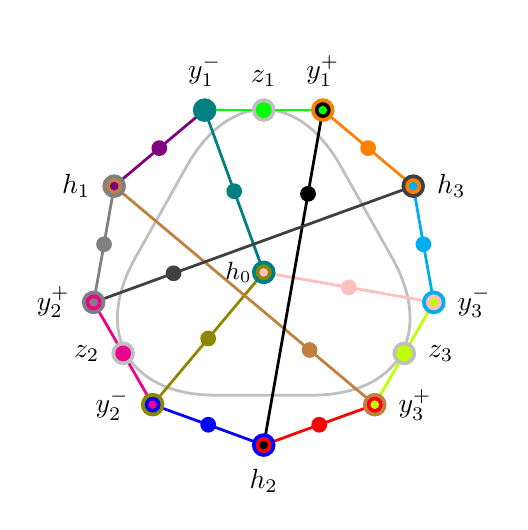
\begin{tikzpicture}  [scale=0.3]

\newdimen\ms
\ms=0.1cm

\tikzstyle{every path}=[line width=1pt]
\tikzstyle{c3}=[circle,inner sep={\ms/8},minimum size=3*\ms]
\tikzstyle{c2}=[circle,inner sep={\ms/8},minimum size=2*\ms]
\tikzstyle{c1}=[circle,inner sep={\ms/8},minimum size=1.1*\ms]



		% Define positions of all observables
		\path
     (-2.50, 6.87    ) coordinate(2)     % $y_1^-
			  (-6.33,   3.65  ) coordinate(4)    % h_1
			  (-7.20, -1.27   ) coordinate(6)       % y_2^+
			  (-4.70, -5.60   ) coordinate(8)       % y_2^-
			  (0, -7.31       ) coordinate(10)       % h_2
			  (4.70, -5.60    ) coordinate(12)        % y_3^+$
     (7.20, -1.27    ) coordinate(14)       % y_3^-
			  (6.33, 3.65     ) coordinate(16)       % h_3
			  (2.50, 6.87     ) coordinate(18)    % y_1^+

			  (0, 6.87        ) coordinate(1)     % $z_1$
			  (-4.42, 5.26    ) coordinate(3)
			  (-6.76, 1.19    ) coordinate(5)
			  (-5.95, -3.43   ) coordinate(7)     % $z_2$
			  (-2.35, -6.45   ) coordinate(9)
     (2.35, -6.45    ) coordinate(11)
			  (5.95,-3.43     ) coordinate(13)    % $z_3$
			  (6.76, 1.19     ) coordinate(15)
		   (4.42, 5.26     ) coordinate(17)

     (0,0) coordinate(19)


(0, 10.3       ) coordinate(20)     % ze1
			  (-8.7, -5.2    ) coordinate(21)     % ze2
			  (8.7,-5.2    ) coordinate(22)    % ze3


     (-1.25, 3.435 ) coordinate(23)
     (3.60, -0.635 ) coordinate(24)
     (-2.35, -2.80 ) coordinate(25)
% h1={-6.33,   3.65  }; h3p={4.70, -5.60    } ; h1d2=  (h1+h3p )/2 ; c1=  (h1d2+h3p )/2
     (1.9425, -3.2875) coordinate(26)
% h2={0, -7.31    }; h1p={2.50, 6.87   } ; h2d2=  (h2+h1p )/2 ; c2=  (h2d2+h1p )/2
     (1.875, 3.325) coordinate(27)
% h3={6.33, 3.65    }; h2p={-7.20, -1.27    } ; h3d2=  (h3+h2p )/2 ; c3=  (h3d2+h2p )/2
     (-3.8175, -0.04) coordinate(28)
;

%(4.70-6.33,   3.65  -5.60   ) coordinate(4)    % h_1

	
		% Draw all the context curves
		
\draw [rounded corners=20mm,color=lightgray]     (20) -- (21) -- (22) --  cycle;


\draw [color=green] (18) -- (1) -- (2);
\draw [color=violet] (2) -- (3) -- (4);
\draw [color=gray] (4) -- (5) -- (6);
\draw [color=magenta] (6) -- (7) -- (8);
\draw [color=blue] (8) -- (9) -- (10);
\draw [color=red] (10) -- (11) -- (12) ;

\draw [color=lime] (12) -- (13) -- (14);
\draw [color=cyan] (14) -- (15) -- (16);
\draw [color=orange] (16) -- (17) -- (18);

\draw [color=teal] (19) -- (2);
\draw [color=olive] (19) -- (8);
\draw [color=pink] (19) -- (14);

\draw [color=brown] (4) -- (12);
\draw [color=black] (10) -- (18);
\draw [color=darkgray] (16) -- (6);





%\draw [color=lightgray](0,0) circle (6.87);



\draw (19) coordinate[c3,fill=teal];
\draw (19) coordinate[c2,fill=olive];
\draw (19) coordinate[c1,fill=pink,label={[xshift=1.5pt]180:{\small $h_0$}}];


\draw (1)  coordinate[c3,fill=lightgray,label=90:$z_1$];
\draw (1)  coordinate[c2,fill=green];

\draw (2)  coordinate[c3,fill=teal,label=90:$y_1^-$];

\draw (3)  coordinate[c2,fill=violet];

\draw (4)  coordinate[c3,fill=gray,label=180:$h_1$];
\draw (4)  coordinate[c2,fill=brown];
\draw (4)  coordinate[c1,fill=violet];

\draw (5)  coordinate[c2,fill=gray,label=0:$ $];

\draw (6)  coordinate[c3,fill=darkgray,fill=gray,label=180:$y_2^+$];
\draw (6)  coordinate[c2,fill=magenta];
\draw (6)  coordinate[c1,fill=gray];

\draw (7)  coordinate[c3,fill=lightgray,label=180:$z_2$];
\draw (7)  coordinate[c2,fill=magenta];

\draw (8)  coordinate[c3,fill=olive,label=180:$y_2^-$];
\draw (8)  coordinate[c2,fill=blue];
\draw (8)  coordinate[c1,fill=magenta];

\draw (9)  coordinate[c2,fill=blue,label=0:$ $];

\draw (10) coordinate[c3,fill=blue,label=270:$h_2$];
\draw (10) coordinate[c2,fill=red];
\draw (10) coordinate[c1,fill=black];

\draw (11) coordinate[c2,fill=red,label=0:$ $];

\draw (12) coordinate[c3,fill=brown,label=0:$y_3^+$];
\draw (12) coordinate[c2,fill=red];
\draw (12) coordinate[c1,fill=lime];

\draw (13) coordinate[c3,fill=lightgray,label=0:$z_3$];
\draw (13) coordinate[c2,fill=lime];

\draw (14) coordinate[c3,fill=cyan,label=0:$y_3^-$];
\draw (14) coordinate[c2,fill=pink];
\draw (14) coordinate[c1,fill=lime];

\draw (15) coordinate[c2,fill=cyan,label=0:$ $];

\draw (16) coordinate[c3,fill=darkgray,label=0:$h_3$];
\draw (16) coordinate[c2,fill=orange];
\draw (16) coordinate[c1,fill=cyan];

\draw (17) coordinate[c2,fill=orange,label=0:$ $];

\draw (18) coordinate[c3,fill=orange,label=90:$y_1^+$];
\draw (18) coordinate[c2,fill=black];
\draw (18) coordinate[c1,fill=green];

\draw (23) coordinate[c2,fill=teal];
\draw (24) coordinate[c2,fill=pink];
\draw (25) coordinate[c2,fill=olive];
\draw (26) coordinate[c2,fill=brown];
\draw (27) coordinate[c2,fill=black];
\draw (28) coordinate[c2,fill=darkgray];


		\end{tikzpicture}
&
\begin{tikzpicture}  [scale=0.4]
\newdimen\ms
\ms=0.1cm

\tikzstyle{every path}=[line width=1pt]
\tikzstyle{c3}=[circle,inner sep={\ms/8},minimum size=3*\ms]
\tikzstyle{c2}=[circle,inner sep={\ms/8},minimum size=2*\ms]
\tikzstyle{c1}=[circle,inner sep={\ms/8},minimum size=1.1*\ms]

% Radius of regular polygons
\newdimen\R
\R=6cm
%\r= { \R * sqrt(3)/2}
\newdimen\K
\K=3cm

% Define positions of all observables
\path
  ({90 + 0 * 360 /5}:\R      ) coordinate(1)
  ({90 + 360 /10 + 0 * 360/5} : {\R * 0.6881/0.8507} ) coordinate(2)
  ({90 + 1 * 360 /5}:\R   ) coordinate(3)
  ({90 + 360 /10 + 1 * 360/5} : {\R * 0.6881/0.8507} ) coordinate(4)
  ({90 + 2 * 360 /5}:\R  ) coordinate(5)
  ({90 + 360 /10 + 2 * 360/5} : {\R * 0.6881/0.8507} ) coordinate(6)
  ({90 + 3 * 360 /5}:\R  ) coordinate(7)
  ({90 + 360 /10 + 3 * 360/5} : {\R * 0.6881/0.8507} ) coordinate(8)
  ({90 + 4 * 360 /5}:\R     ) coordinate(9)
  ({90 + 360 /10 + 4 * 360/5} : {\R * 0.6881/0.8507} ) coordinate(10)
  ({90 + 0 * 360 /5}:\K      ) coordinate(11)
  ({90 + 360 /10 + 0 * 360/5} : {\K * 0.6881/0.8507} ) coordinate(12)
  ({90 + 1 * 360 /5}:\K   ) coordinate(13)
  ({90 + 360 /10 + 1 * 360/5} : {\K * 0.6881/0.8507} ) coordinate(14)
  ({90 + 2 * 360 /5}:\K  ) coordinate(15)
  ({90 + 360 /10 + 2 * 360/5} : {\K * 0.6881/0.8507} ) coordinate(16)
  ({90 + 3 * 360 /5}:\K  ) coordinate(17)
  ({90 + 360 /10 + 3 * 360/5} : {\R * 0.6881/0.8507} ) coordinate(18)
  ({90 + 4 * 360 /5}:\K     ) coordinate(19)
  ({90 + 360 /10 + 4 * 360/5} : {\K * 0.6881/0.8507} ) coordinate(20)

  ({90 + 2 * 360 /5}:{(\R+\K)/2}) coordinate(21)

;

% draw contexts

\draw [color=orange] (1) -- (2) -- (3);
\draw [color=darkgray] (3) -- (4) -- (5);
\draw [color=gray] (5) -- (6) -- (7);
\draw [color=violet] (7) -- (8) -- (9);
\draw [color=green] (9) -- (10) -- (1);    %

\draw [color=blue] (11) -- (15) ;
\draw [color=olive] (15) -- (19);
\draw [color=pink] (19) -- (13);
\draw [color=lime] (13) -- (17);
\draw [color=red] (17) -- (11);

\draw ($ (11) !.5! (15) $) coordinate[c2,fill=blue];  %
\draw ($ (15) !.5! (19) $) coordinate[c2,fill=olive];  %
\draw ($ (19) !.47! (13) $) coordinate[c2,fill=pink];  %
\draw ($ (17) !.5! (11) $) coordinate[c2,fill=red];  %

\draw [color=black] (1) -- (11);
\draw [color=cyan] (3) -- (13);
\draw [color=magenta] (5) -- (15);
\draw [color=brown] (7) -- (17);
\draw [color=teal] (9) -- (19);

\draw ($ (1) !.5! (11) $) coordinate[c2,fill=black];  %
\draw ($ (3) !.5! (13) $) coordinate[c2,fill=cyan];  %
\draw ($ (7) !.5! (17) $) coordinate[c2,fill=brown];  %
\draw ($ (9) !.5! (19) $) coordinate[c2,fill=teal];  %

\draw [color=lightgray] (10)  to   [out=-140,in=100] ($ (13) !.5! (17) $)  to   [out=-90,in=0] (21);
%
%%
%% draw atoms
%%
%
\draw (1) coordinate[c3,fill=black,label=90:$y_1^+$];  %
\draw (1) coordinate[c2,fill=green];   %
\draw (1) coordinate[c1,fill=orange];  %
%
\draw (2) coordinate[c2,fill=orange];    %
%
\draw (3) coordinate[c3,fill=cyan,label=180:$h_3$];   %
\draw (3) coordinate[c2,fill=darkgray]; %
\draw (3) coordinate[c1,fill=orange];  %
%
\draw (4) coordinate[c2,fill=darkgray];  %
%
\draw (5) coordinate[c3,fill=magenta,label=270:$y_2^+$];  %
\draw (5) coordinate[c2,fill=gray];  %
\draw (5) coordinate[c1,fill=darkgray];  %
%
\draw (6) coordinate[c2,fill=gray];
%
\draw (7) coordinate[c3,fill=brown,label=270:$h_1$];  %
\draw (7) coordinate[c2,fill=violet];  %
\draw (7) coordinate[c1,fill=gray];  %
%
\draw (8) coordinate[c2,fill=violet];  %
%
\draw (9) coordinate[c3,fill=green,label=0:$y_1^-$];
%
\draw (10) coordinate[c2,fill=green,label=0:$z_1$];  %
\draw (10) coordinate[c1,fill=lightgray];  %
%
\draw (11) coordinate[c3,fill=black,label=180:$h_2$];  %
\draw (11) coordinate[c2,fill=red];  %
\draw (11) coordinate[c1,fill=blue]; %
%
%
\draw (13) coordinate[c3,fill=cyan,label=90:$y_3^-$]; %
\draw (13) coordinate[c2,fill=lime];  %
\draw (13) coordinate[c1,fill=pink];  %
%
\draw (15) coordinate[c3,fill=magenta,label=180:$y_2^-$]; %
\draw (15) coordinate[c2,fill=olive]; %
\draw (15) coordinate[c1,fill=blue]; %

\draw (17) coordinate[c3,fill=brown,label=0:$y_3^+$];  %
\draw (17) coordinate[c2,fill=red];   %
\draw (17) coordinate[c1,fill=lime]; %

\draw (19) coordinate[c3,fill=teal,label=90:$h_0$]; %
\draw (19) coordinate[c2,fill=pink]; %
\draw (19) coordinate[c1,fill=olive]; %

%
\draw (21) coordinate[c2,fill=magenta];  %
\draw (21) coordinate[c1,fill=lightgray,label=-15:$z_2$];  %

\draw ($ (13) !.5! (17) $) coordinate[c2,fill=lightgray];  %
\draw ($ (13) !.5! (17) $) coordinate[c1,fill=lime,label=45:$z_3$];  %


\end{tikzpicture}
\\
(a)&(b)
\end{tabular}
\end{center}
\caption{\label{2017-b-f-Yu-2012} (Color online) Redraw~\cite[Chapter~12, p.~92]{svozil-pac} of two equivalent representations (a) and (b) of a Petersen graph-like
(with one additional context connecting
$z_1$,
$z_2$, and
$z_3$)
hypergraph of the logic considered by Yu and Oh~\cite[Fig.~2]{Yu-2012}.
The set of two-valued states enforces at most one of the four atoms $h_0$, $h_1$, $h_2$, $h_3$ to be 1.
The logic has a (quantum) realization in $\mathbb{R}^3$
consisting of the 25 projections;  associated with the one dimensional subspaces
spanned by  the 13 vectors from the origin $\left(0,0,0\right)^\intercal$ to
$z_1 = \left( 1, 0, 0 \right)^\intercal $,
$z_2 = \left( 0, 1, 0 \right)^\intercal $,
$z_3 = \left( 0, 0, 1 \right)^\intercal $,
$y^-_1 = \left( 0, 1, -1 \right)^\intercal $,
$y^-_2 = \left( 1, 0, -1 \right)^\intercal $,
$y^-_3 = \left( 1, -1, 0 \right)^\intercal $,
$y^+_1 = \left( 0, 1, 1 \right)^\intercal $,
$y^+_2 = \left( 1, 0, 1 \right)^\intercal $,
$y^+_3 = \left( 1, 1, 0 \right)^\intercal $,
$h_0 = \left( 1, 1, 1 \right)^\intercal $,
$h_1 = \left( -1, 1, 1 \right)^\intercal $,
$h_2 = \left( 1, -1, 1 \right)^\intercal $,
$h_3 = \left( 1, 1, -1 \right)^\intercal $,
respectively~\cite{Yu-2012}.
}
\end{figure*}

Without loss of generality, we can assume $h_0$ is red.
Then, $y_1^-$, $y_2^-$, and $y_3^-$ must be either green or blue.

Assuming all are colored green leads to a contradiction, as the context $\{z_1,z_2,z_3\}$ would then lack the color green.

Therefore, at least one of $y_1^-$, $y_2^-$, and $y_3^-$ must be colored differently.
By symmetry, without loss of generality, let $y_1^-$ and $y_2^-$ be green, and $y_3^-$ be blue, as depicted in Figures~\ref{2025-b-f-Yu-2012-c1} and~\ref{2025-b-f-Yu-2012-c2}, (a) and (b), respectively.
Then, $z_1$ as well as $z_2$ cannot be green, and $z_3$ cannot be blue.

\subsection*{Case 1}

Suppose that $z_1$ is red.
Then, $z_2$ must be blue, and $z_3$ must be green, as depicted in Figure~\ref{2025-b-f-Yu-2012-c1}(c) and (d).
We can now assign colors to the three contexts
$\{
y_1^+ , y_1^- , z_1
\}$,
$\{
y_2^+ , y_2^- , z_2
\}$, and
$\{
y_3^+ , y_3^- , z_3
\}$
by assigning
blue to $y_1^+$,
red to $y_2^+$, and
red to $y_3^+$, respectively, as depicted in Figure~\ref{2025-b-f-Yu-2012-c1}(e) and (f).

Consequently, $h_2$ cannot be red because $y_3^+$ is red, nor green, as $y_2^-$ is green,
nor blue as $y_1^+$ is blue,
and all $y_3^+$, $y_2^-$, and $y_1^+$ are adjacent to $h_2$.

\subsection*{Case 2}

Suppose that $z_1$ is blue.
Then $z_2$ must be red, and $z_3$ must be green, as depicted in Figure~\ref{2025-b-f-Yu-2012-c2}(c) and (d).

Consequently, $y_1^+$ must be red, $y_2^+$ must be blue, and $y_3^+$ must be red.
Additionally, $h_3$ must be green, and $h_2$ must be blue.
As before, we can now assign colors to the three contexts
$\{
y_1^+ , y_1^- , z_1
\}$,
$\{
y_2^+ , y_2^- , z_2
\}$, and
$\{
y_3^+ , y_3^- , z_3
\}$
by assigning
red to $y_1^+$ and $y_3^+$, and
blue to $y_2^+$, respectively, as depicted in Figure~\ref{2025-b-f-Yu-2012-c2}(e) and (f)..

Now $h_1$ cannot be red because $y_3^+$ is red, nor green, as $y_1^-$ is green, nor blue as $y_2^+$ is blue,
and all $y_3^+$, $y_1^-$, and $y_2^+$ are adjacent to $h_1$.

It is not difficult to work out a coloring of the Yu-Oh hypergraph with four colors.
Therefore, its chromatic number is 4.
In passing, we note that it has a separating set of 24 two-valued measures.


%\newpage

\begin{figure*}
\begin{center}
\begin{tabular}{cc}
		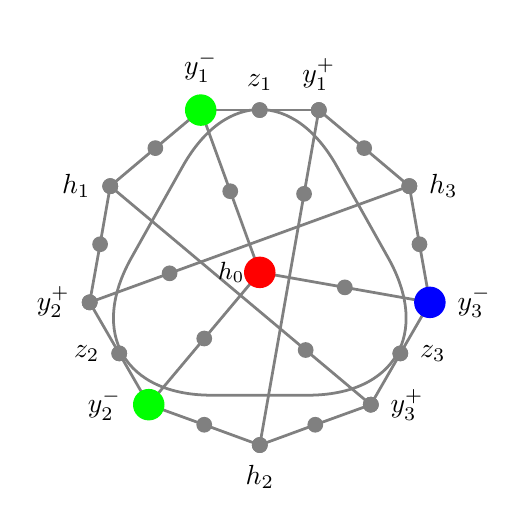
\begin{tikzpicture}  [scale=0.3]

\newdimen\ms
\ms=0.1cm

\tikzstyle{every path}=[line width=1pt]
\tikzstyle{c4}=[circle,inner sep={\ms/8},minimum size=4*\ms]
\tikzstyle{c3}=[circle,inner sep={\ms/8},minimum size=3*\ms]
\tikzstyle{c2}=[circle,inner sep={\ms/8},minimum size=2*\ms]
\tikzstyle{c1}=[circle,inner sep={\ms/8},minimum size=1.1*\ms]



		% Define positions of all observables
		\path
     (-2.50, 6.87    ) coordinate(2)     % $y_1^-
			  (-6.33,   3.65  ) coordinate(4)    % h_1
			  (-7.20, -1.27   ) coordinate(6)       % y_2^+
			  (-4.70, -5.60   ) coordinate(8)       % y_2^-
			  (0, -7.31       ) coordinate(10)       % h_2
			  (4.70, -5.60    ) coordinate(12)        % y_3^+$
     (7.20, -1.27    ) coordinate(14)       % y_3^-
			  (6.33, 3.65     ) coordinate(16)       % h_3
			  (2.50, 6.87     ) coordinate(18)    % y_1^+

			  (0, 6.87        ) coordinate(1)     % $z_1$
			  (-4.42, 5.26    ) coordinate(3)
			  (-6.76, 1.19    ) coordinate(5)
			  (-5.95, -3.43   ) coordinate(7)     % $z_2$
			  (-2.35, -6.45   ) coordinate(9)
     (2.35, -6.45    ) coordinate(11)
			  (5.95,-3.43     ) coordinate(13)    % $z_3$
			  (6.76, 1.19     ) coordinate(15)
		   (4.42, 5.26     ) coordinate(17)

     (0,0) coordinate(19)


(0, 10.3       ) coordinate(20)     % ze1
			  (-8.7, -5.2    ) coordinate(21)     % ze2
			  (8.7,-5.2    ) coordinate(22)    % ze3


     (-1.25, 3.435 ) coordinate(23)
     (3.60, -0.635 ) coordinate(24)
     (-2.35, -2.80 ) coordinate(25)
% h1={-6.33,   3.65  }; h3p={4.70, -5.60    } ; h1d2=  (h1+h3p )/2 ; c1=  (h1d2+h3p )/2
     (1.9425, -3.2875) coordinate(26)
% h2={0, -7.31    }; h1p={2.50, 6.87   } ; h2d2=  (h2+h1p )/2 ; c2=  (h2d2+h1p )/2
     (1.875, 3.325) coordinate(27)
% h3={6.33, 3.65    }; h2p={-7.20, -1.27    } ; h3d2=  (h3+h2p )/2 ; c3=  (h3d2+h2p )/2
     (-3.8175, -0.04) coordinate(28)
;

%(4.70-6.33,   3.65  -5.60   ) coordinate(4)    % h_1

	
		% Draw all the context curves
		
\draw [rounded corners=20mm,color=gray]     (20) -- (21) -- (22) --  cycle;


\draw [color=gray] (18) -- (1) -- (2);
\draw [color=gray] (2) -- (3) -- (4);
\draw [color=gray] (4) -- (5) -- (6);
\draw [color=gray] (6) -- (7) -- (8);
\draw [color=gray] (8) -- (9) -- (10);
\draw [color=gray] (10) -- (11) -- (12) ;

\draw [color=gray] (12) -- (13) -- (14);
\draw [color=gray] (14) -- (15) -- (16);
\draw [color=gray] (16) -- (17) -- (18);

\draw [color=gray] (19) -- (2);
\draw [color=gray] (19) -- (8);
\draw [color=gray] (19) -- (14);

\draw [color=gray] (4) -- (12);
\draw [color=gray] (10) -- (18);
\draw [color=gray] (16) -- (6);





%\draw [color=gray](0,0) circle (6.87);



\draw (19) coordinate[c4,fill=red,label={[xshift=4.5pt]180:{\small $h_0$}}];


\draw (1)  coordinate[c2,fill=gray,label=90:$z_1$];
\draw (1)  coordinate[c2,fill=gray];

\draw (2)  coordinate[c4,fill=green,label=90:$y_1^-$];

\draw (3)  coordinate[c2,fill=gray];

\draw (4)  coordinate[c2,fill=gray,label=180:$h_1$];
\draw (4)  coordinate[c2,fill=gray];
\draw (4)  coordinate[c2,fill=gray];

\draw (5)  coordinate[c2,fill=gray,label=0:$ $];

\draw (6)  coordinate[c2,fill=gray,fill=gray,label=180:$y_2^+$];
\draw (6)  coordinate[c2,fill=gray];
\draw (6)  coordinate[c2,fill=gray];

\draw (7)  coordinate[c2,fill=gray,label=180:$z_2$];
\draw (7)  coordinate[c2,fill=gray];

\draw (8)  coordinate[c4,fill=green,label=180:$y_2^-$];

\draw (9)  coordinate[c2,fill=gray,label=0:$ $];

\draw (10) coordinate[c2,fill=gray,label=270:$h_2$];
\draw (10) coordinate[c2,fill=gray];
\draw (10) coordinate[c2,fill=gray];

\draw (11) coordinate[c2,fill=gray,label=0:$ $];

\draw (12) coordinate[c2,fill=gray,label=0:$y_3^+$];
\draw (12) coordinate[c2,fill=gray];
\draw (12) coordinate[c2,fill=gray];

\draw (13) coordinate[c2,fill=gray,label=0:$z_3$];
\draw (13) coordinate[c2,fill=gray];

\draw (14) coordinate[c4,fill=blue,label=0:$y_3^-$];

\draw (15) coordinate[c2,fill=gray,label=0:$ $];

\draw (16) coordinate[c2,fill=gray,label=0:$h_3$];
\draw (16) coordinate[c2,fill=gray];
\draw (16) coordinate[c2,fill=gray];

\draw (17) coordinate[c2,fill=gray,label=0:$ $];

\draw (18) coordinate[c2,fill=gray,label=90:$y_1^+$];
\draw (18) coordinate[c2,fill=gray];
\draw (18) coordinate[c2,fill=gray];

\draw (23) coordinate[c2,fill=gray];
\draw (24) coordinate[c2,fill=gray];
\draw (25) coordinate[c2,fill=gray];
\draw (26) coordinate[c2,fill=gray];
\draw (27) coordinate[c2,fill=gray];
\draw (28) coordinate[c2,fill=gray];


		\end{tikzpicture}
&
\begin{tikzpicture}  [scale=0.4]
\newdimen\ms
\ms=0.1cm

\tikzstyle{every path}=[line width=1pt]
\tikzstyle{c4}=[circle,inner sep={\ms/8},minimum size=4*\ms]
\tikzstyle{c3}=[circle,inner sep={\ms/8},minimum size=3*\ms]
\tikzstyle{c2}=[circle,inner sep={\ms/8},minimum size=2*\ms]
\tikzstyle{c1}=[circle,inner sep={\ms/8},minimum size=1.1*\ms]

% Radius of regular polygons
\newdimen\R
\R=6cm
%\r= { \R * sqrt(3)/2}
\newdimen\K
\K=3cm

% Define positions of all observables
\path
  ({90 + 0 * 360 /5}:\R      ) coordinate(1)
  ({90 + 360 /10 + 0 * 360/5} : {\R * 0.6881/0.8507} ) coordinate(2)
  ({90 + 1 * 360 /5}:\R   ) coordinate(3)
  ({90 + 360 /10 + 1 * 360/5} : {\R * 0.6881/0.8507} ) coordinate(4)
  ({90 + 2 * 360 /5}:\R  ) coordinate(5)
  ({90 + 360 /10 + 2 * 360/5} : {\R * 0.6881/0.8507} ) coordinate(6)
  ({90 + 3 * 360 /5}:\R  ) coordinate(7)
  ({90 + 360 /10 + 3 * 360/5} : {\R * 0.6881/0.8507} ) coordinate(8)
  ({90 + 4 * 360 /5}:\R     ) coordinate(9)
  ({90 + 360 /10 + 4 * 360/5} : {\R * 0.6881/0.8507} ) coordinate(10)
  ({90 + 0 * 360 /5}:\K      ) coordinate(11)
  ({90 + 360 /10 + 0 * 360/5} : {\K * 0.6881/0.8507} ) coordinate(12)
  ({90 + 1 * 360 /5}:\K   ) coordinate(13)
  ({90 + 360 /10 + 1 * 360/5} : {\K * 0.6881/0.8507} ) coordinate(14)
  ({90 + 2 * 360 /5}:\K  ) coordinate(15)
  ({90 + 360 /10 + 2 * 360/5} : {\K * 0.6881/0.8507} ) coordinate(16)
  ({90 + 3 * 360 /5}:\K  ) coordinate(17)
  ({90 + 360 /10 + 3 * 360/5} : {\R * 0.6881/0.8507} ) coordinate(18)
  ({90 + 4 * 360 /5}:\K     ) coordinate(19)
  ({90 + 360 /10 + 4 * 360/5} : {\K * 0.6881/0.8507} ) coordinate(20)

  ({90 + 2 * 360 /5}:{(\R+\K)/2}) coordinate(21)

;

% draw contexts

\draw [color=gray] (1) -- (2) -- (3);
\draw [color=gray] (3) -- (4) -- (5);
\draw [color=gray] (5) -- (6) -- (7);
\draw [color=gray] (7) -- (8) -- (9);
\draw [color=gray] (9) -- (10) -- (1);    %

\draw [color=gray] (11) -- (15) ;
\draw [color=gray] (15) -- (19);
\draw [color=gray] (19) -- (13);
\draw [color=gray] (13) -- (17);
\draw [color=gray] (17) -- (11);

\draw ($ (11) !.5! (15) $) coordinate[c2,fill=gray];  %
\draw ($ (15) !.5! (19) $) coordinate[c2,fill=gray];  %
\draw ($ (19) !.47! (13) $) coordinate[c2,fill=gray];  %
\draw ($ (17) !.5! (11) $) coordinate[c2,fill=gray];  %

\draw [color=gray] (1) -- (11);
\draw [color=gray] (3) -- (13);
\draw [color=gray] (5) -- (15);
\draw [color=gray] (7) -- (17);
\draw [color=gray] (9) -- (19);

\draw ($ (1) !.5! (11) $) coordinate[c2,fill=gray];  %
\draw ($ (3) !.5! (13) $) coordinate[c2,fill=gray];  %
\draw ($ (7) !.5! (17) $) coordinate[c2,fill=gray];  %
\draw ($ (9) !.5! (19) $) coordinate[c2,fill=gray];  %

\draw [color=gray] (10)  to   [out=-140,in=100] ($ (13) !.5! (17) $)  to   [out=-90,in=0] (21);
%
%%
%% draw atoms
%%
%
\draw (1) coordinate[c2,fill=gray,label=90:$y_1^+$];  %
\draw (1) coordinate[c2,fill=gray];   %
\draw (1) coordinate[c2,fill=gray];  %
%
\draw (2) coordinate[c2,fill=gray];    %
%
\draw (3) coordinate[c2,fill=gray,label=180:$h_3$];   %
\draw (3) coordinate[c2,fill=gray]; %
\draw (3) coordinate[c2,fill=gray];  %
%
\draw (4) coordinate[c2,fill=gray];  %
%
\draw (5) coordinate[c2,fill=gray,label=270:$y_2^+$];  %
\draw (5) coordinate[c2,fill=gray];  %
\draw (5) coordinate[c2,fill=gray];  %
%
\draw (6) coordinate[c2,fill=gray];
%
\draw (7) coordinate[c2,fill=gray,label=270:$h_1$];  %
\draw (7) coordinate[c2,fill=gray];  %
\draw (7) coordinate[c2,fill=gray];  %
%
\draw (8) coordinate[c2,fill=gray];  %
%
\draw (9) coordinate[c4,fill=green,label=0:$y_1^-$];
%
\draw (10) coordinate[c2,fill=gray,label=0:$z_1$];  %
\draw (10) coordinate[c2,fill=gray];  %
%
\draw (11) coordinate[c2,fill=gray,label=180:$h_2$];  %
\draw (11) coordinate[c2,fill=gray];  %
\draw (11) coordinate[c2,fill=gray]; %
%
%
\draw (13) coordinate[c4,fill=blue,label=90:$y_3^-$]; %
%
\draw (15) coordinate[c4,fill=green,label=180:$y_2^-$]; %

\draw (17) coordinate[c2,fill=gray,label=0:$y_3^+$];  %
\draw (17) coordinate[c2,fill=gray];   %
\draw (17) coordinate[c2,fill=gray]; %

\draw (19) coordinate[c4,fill=red,label=90:$h_0$]; %

%
\draw (21) coordinate[c2,fill=gray];  %
\draw (21) coordinate[c2,fill=gray,label=-15:$z_2$];  %

\draw ($ (13) !.5! (17) $) coordinate[c2,fill=gray];  %
\draw ($ (13) !.5! (17) $) coordinate[c2,fill=gray,label=45:$z_3$];  %


\end{tikzpicture}
\\
(a)&(b)
\\
%%%%%%%%%%%%%%%%%%%%%%%%%%%%%%%%%%%%%%%%%%%%%%%%%%%%%%%%%%%%%%%%%%%%%%%%%%%%%%%%%%%%%%%%%%%5
%%%%%%%%%%%%%%%%%%%%%%%%%%%%%%%%%%%%%%%%%%%%%%%%%%%%%%%%%%%%%%%%%%%%%%%%%%%%%%%%%%%%%%%%%%%5
%%%%%%%%%%%%%%%%%%%%%%%%%%%%%%%%%%%%%%%%%%%%%%%%%%%%%%%%%%%%%%%%%%%%%%%%%%%%%%%%%%%%%%%%%%%5
%%%%%%%%%%%%%%%%%%%%%%%%%%%%%%%%%%%%%%%%%%%%%%%%%%%%%%%%%%%%%%%%%%%%%%%%%%%%%%%%%%%%%%%%%%%5
%%%%%%%%%%%%%%%%%%%%%%%%%%%%%%%%%%%%%%%%%%%%%%%%%%%%%%%%%%%%%%%%%%%%%%%%%%%%%%%%%%%%%%%%%%%5
		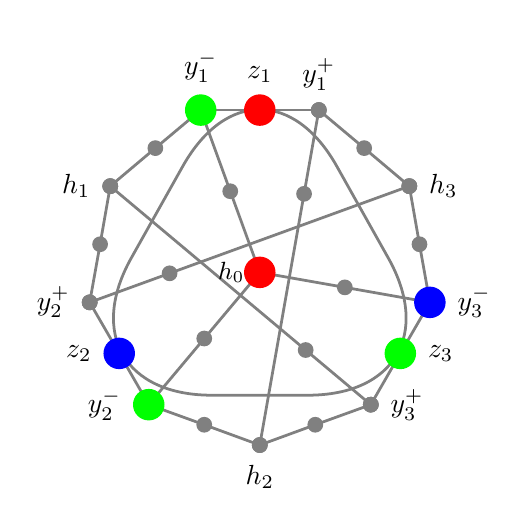
\begin{tikzpicture}  [scale=0.3]

\newdimen\ms
\ms=0.1cm

\tikzstyle{every path}=[line width=1pt]
\tikzstyle{c4}=[circle,inner sep={\ms/8},minimum size=4*\ms]
\tikzstyle{c3}=[circle,inner sep={\ms/8},minimum size=3*\ms]
\tikzstyle{c2}=[circle,inner sep={\ms/8},minimum size=2*\ms]
\tikzstyle{c1}=[circle,inner sep={\ms/8},minimum size=1.1*\ms]



		% Define positions of all observables
		\path
     (-2.50, 6.87    ) coordinate(2)     % $y_1^-
			  (-6.33,   3.65  ) coordinate(4)    % h_1
			  (-7.20, -1.27   ) coordinate(6)       % y_2^+
			  (-4.70, -5.60   ) coordinate(8)       % y_2^-
			  (0, -7.31       ) coordinate(10)       % h_2
			  (4.70, -5.60    ) coordinate(12)        % y_3^+$
     (7.20, -1.27    ) coordinate(14)       % y_3^-
			  (6.33, 3.65     ) coordinate(16)       % h_3
			  (2.50, 6.87     ) coordinate(18)    % y_1^+

			  (0, 6.87        ) coordinate(1)     % $z_1$
			  (-4.42, 5.26    ) coordinate(3)
			  (-6.76, 1.19    ) coordinate(5)
			  (-5.95, -3.43   ) coordinate(7)     % $z_2$
			  (-2.35, -6.45   ) coordinate(9)
     (2.35, -6.45    ) coordinate(11)
			  (5.95,-3.43     ) coordinate(13)    % $z_3$
			  (6.76, 1.19     ) coordinate(15)
		   (4.42, 5.26     ) coordinate(17)

     (0,0) coordinate(19)


(0, 10.3       ) coordinate(20)     % ze1
			  (-8.7, -5.2    ) coordinate(21)     % ze2
			  (8.7,-5.2    ) coordinate(22)    % ze3


     (-1.25, 3.435 ) coordinate(23)
     (3.60, -0.635 ) coordinate(24)
     (-2.35, -2.80 ) coordinate(25)
% h1={-6.33,   3.65  }; h3p={4.70, -5.60    } ; h1d2=  (h1+h3p )/2 ; c1=  (h1d2+h3p )/2
     (1.9425, -3.2875) coordinate(26)
% h2={0, -7.31    }; h1p={2.50, 6.87   } ; h2d2=  (h2+h1p )/2 ; c2=  (h2d2+h1p )/2
     (1.875, 3.325) coordinate(27)
% h3={6.33, 3.65    }; h2p={-7.20, -1.27    } ; h3d2=  (h3+h2p )/2 ; c3=  (h3d2+h2p )/2
     (-3.8175, -0.04) coordinate(28)
;

%(4.70-6.33,   3.65  -5.60   ) coordinate(4)    % h_1

	
		% Draw all the context curves
		
\draw [rounded corners=20mm,color=gray]     (20) -- (21) -- (22) --  cycle;


\draw [color=gray] (18) -- (1) -- (2);
\draw [color=gray] (2) -- (3) -- (4);
\draw [color=gray] (4) -- (5) -- (6);
\draw [color=gray] (6) -- (7) -- (8);
\draw [color=gray] (8) -- (9) -- (10);
\draw [color=gray] (10) -- (11) -- (12) ;

\draw [color=gray] (12) -- (13) -- (14);
\draw [color=gray] (14) -- (15) -- (16);
\draw [color=gray] (16) -- (17) -- (18);

\draw [color=gray] (19) -- (2);
\draw [color=gray] (19) -- (8);
\draw [color=gray] (19) -- (14);

\draw [color=gray] (4) -- (12);
\draw [color=gray] (10) -- (18);
\draw [color=gray] (16) -- (6);





%\draw [color=gray](0,0) circle (6.87);



\draw (19) coordinate[c4,fill=red,label={[xshift=4.5pt]180:{\small $h_0$}}];


\draw (1)  coordinate[c4,fill=red,label=90:$z_1$];

\draw (2)  coordinate[c4,fill=green,label=90:$y_1^-$];

\draw (3)  coordinate[c2,fill=gray];

\draw (4)  coordinate[c2,fill=gray,label=180:$h_1$];
\draw (4)  coordinate[c2,fill=gray];
\draw (4)  coordinate[c2,fill=gray];

\draw (5)  coordinate[c2,fill=gray,label=0:$ $];

\draw (6)  coordinate[c2,fill=gray,fill=gray,label=180:$y_2^+$];
\draw (6)  coordinate[c2,fill=gray];
\draw (6)  coordinate[c2,fill=gray];

\draw (7)  coordinate[c4,fill=blue,label=180:$z_2$];

\draw (8)  coordinate[c4,fill=green,label=180:$y_2^-$];

\draw (9)  coordinate[c2,fill=gray,label=0:$ $];

\draw (10) coordinate[c2,fill=gray,label=270:$h_2$];
\draw (10) coordinate[c2,fill=gray];
\draw (10) coordinate[c2,fill=gray];

\draw (11) coordinate[c2,fill=gray,label=0:$ $];

\draw (12) coordinate[c2,fill=gray,label=0:$y_3^+$];
\draw (12) coordinate[c2,fill=gray];
\draw (12) coordinate[c2,fill=gray];

\draw (13) coordinate[c4,fill=green,label=0:$z_3$];

\draw (14) coordinate[c4,fill=blue,label=0:$y_3^-$];

\draw (15) coordinate[c2,fill=gray,label=0:$ $];

\draw (16) coordinate[c2,fill=gray,label=0:$h_3$];
\draw (16) coordinate[c2,fill=gray];
\draw (16) coordinate[c2,fill=gray];

\draw (17) coordinate[c2,fill=gray,label=0:$ $];

\draw (18) coordinate[c2,fill=gray,label=90:$y_1^+$];
\draw (18) coordinate[c2,fill=gray];
\draw (18) coordinate[c2,fill=gray];

\draw (23) coordinate[c2,fill=gray];
\draw (24) coordinate[c2,fill=gray];
\draw (25) coordinate[c2,fill=gray];
\draw (26) coordinate[c2,fill=gray];
\draw (27) coordinate[c2,fill=gray];
\draw (28) coordinate[c2,fill=gray];


		\end{tikzpicture}
&
\begin{tikzpicture}  [scale=0.4]
\newdimen\ms
\ms=0.1cm

\tikzstyle{every path}=[line width=1pt]
\tikzstyle{c4}=[circle,inner sep={\ms/8},minimum size=4*\ms]
\tikzstyle{c3}=[circle,inner sep={\ms/8},minimum size=3*\ms]
\tikzstyle{c2}=[circle,inner sep={\ms/8},minimum size=2*\ms]
\tikzstyle{c1}=[circle,inner sep={\ms/8},minimum size=1.1*\ms]

% Radius of regular polygons
\newdimen\R
\R=6cm
%\r= { \R * sqrt(3)/2}
\newdimen\K
\K=3cm

% Define positions of all observables
\path
  ({90 + 0 * 360 /5}:\R      ) coordinate(1)
  ({90 + 360 /10 + 0 * 360/5} : {\R * 0.6881/0.8507} ) coordinate(2)
  ({90 + 1 * 360 /5}:\R   ) coordinate(3)
  ({90 + 360 /10 + 1 * 360/5} : {\R * 0.6881/0.8507} ) coordinate(4)
  ({90 + 2 * 360 /5}:\R  ) coordinate(5)
  ({90 + 360 /10 + 2 * 360/5} : {\R * 0.6881/0.8507} ) coordinate(6)
  ({90 + 3 * 360 /5}:\R  ) coordinate(7)
  ({90 + 360 /10 + 3 * 360/5} : {\R * 0.6881/0.8507} ) coordinate(8)
  ({90 + 4 * 360 /5}:\R     ) coordinate(9)
  ({90 + 360 /10 + 4 * 360/5} : {\R * 0.6881/0.8507} ) coordinate(10)
  ({90 + 0 * 360 /5}:\K      ) coordinate(11)
  ({90 + 360 /10 + 0 * 360/5} : {\K * 0.6881/0.8507} ) coordinate(12)
  ({90 + 1 * 360 /5}:\K   ) coordinate(13)
  ({90 + 360 /10 + 1 * 360/5} : {\K * 0.6881/0.8507} ) coordinate(14)
  ({90 + 2 * 360 /5}:\K  ) coordinate(15)
  ({90 + 360 /10 + 2 * 360/5} : {\K * 0.6881/0.8507} ) coordinate(16)
  ({90 + 3 * 360 /5}:\K  ) coordinate(17)
  ({90 + 360 /10 + 3 * 360/5} : {\R * 0.6881/0.8507} ) coordinate(18)
  ({90 + 4 * 360 /5}:\K     ) coordinate(19)
  ({90 + 360 /10 + 4 * 360/5} : {\K * 0.6881/0.8507} ) coordinate(20)

  ({90 + 2 * 360 /5}:{(\R+\K)/2}) coordinate(21)

;

% draw contexts

\draw [color=gray] (1) -- (2) -- (3);
\draw [color=gray] (3) -- (4) -- (5);
\draw [color=gray] (5) -- (6) -- (7);
\draw [color=gray] (7) -- (8) -- (9);
\draw [color=gray] (9) -- (10) -- (1);    %

\draw [color=gray] (11) -- (15) ;
\draw [color=gray] (15) -- (19);
\draw [color=gray] (19) -- (13);
\draw [color=gray] (13) -- (17);
\draw [color=gray] (17) -- (11);

\draw ($ (11) !.5! (15) $) coordinate[c2,fill=gray];  %
\draw ($ (15) !.5! (19) $) coordinate[c2,fill=gray];  %
\draw ($ (19) !.47! (13) $) coordinate[c2,fill=gray];  %
\draw ($ (17) !.5! (11) $) coordinate[c2,fill=gray];  %

\draw [color=gray] (1) -- (11);
\draw [color=gray] (3) -- (13);
\draw [color=gray] (5) -- (15);
\draw [color=gray] (7) -- (17);
\draw [color=gray] (9) -- (19);

\draw ($ (1) !.5! (11) $) coordinate[c2,fill=gray];  %
\draw ($ (3) !.5! (13) $) coordinate[c2,fill=gray];  %
\draw ($ (7) !.5! (17) $) coordinate[c2,fill=gray];  %
\draw ($ (9) !.5! (19) $) coordinate[c2,fill=gray];  %

\draw [color=gray] (10)  to   [out=-140,in=100] ($ (13) !.5! (17) $)  to   [out=-90,in=0] (21);
%
%%
%% draw atoms
%%
%
\draw (1) coordinate[c2,fill=gray,label=90:$y_1^+$];  %
\draw (1) coordinate[c2,fill=gray];   %
\draw (1) coordinate[c2,fill=gray];  %
%
\draw (2) coordinate[c2,fill=gray];    %
%
\draw (3) coordinate[c2,fill=gray,label=180:$h_3$];   %
\draw (3) coordinate[c2,fill=gray]; %
\draw (3) coordinate[c2,fill=gray];  %
%
\draw (4) coordinate[c2,fill=gray];  %
%
\draw (5) coordinate[c2,fill=gray,label=270:$y_2^+$];  %
\draw (5) coordinate[c2,fill=gray];  %
\draw (5) coordinate[c2,fill=gray];  %
%
\draw (6) coordinate[c2,fill=gray];
%
\draw (7) coordinate[c2,fill=gray,label=270:$h_1$];  %
\draw (7) coordinate[c2,fill=gray];  %
\draw (7) coordinate[c2,fill=gray];  %
%
\draw (8) coordinate[c2,fill=gray];  %
%
\draw (9) coordinate[c4,fill=green,label=0:$y_1^-$];
%
\draw (10) coordinate[c4,fill=red,label=0:$z_1$];  %
%
\draw (11) coordinate[c2,fill=gray,label=180:$h_2$];  %
\draw (11) coordinate[c2,fill=gray];  %
\draw (11) coordinate[c2,fill=gray]; %
%
%
\draw (13) coordinate[c4,fill=blue,label=90:$y_3^-$]; %
%
\draw (15) coordinate[c4,fill=green,label=180:$y_2^-$]; %

\draw (17) coordinate[c2,fill=gray,label=0:$y_3^+$];  %
\draw (17) coordinate[c2,fill=gray];   %
\draw (17) coordinate[c2,fill=gray]; %

\draw (19) coordinate[c4,fill=red,label=90:$h_0$]; %

%
\draw (21) coordinate[c4,fill=blue,label=-15:$z_2$];  %

\draw ($ (13) !.5! (17) $) coordinate[c4,fill=green,label=45:$z_3$];  %


\end{tikzpicture}
\\
(c)&(d)
\\
%%%%%%%%%%%%%%%%%%%%%%%%%%%%%%%%%%%%%%%%%%%%%%%%%%%%%%%%%%%%%%%%%%%%%%%%%%%%%%%%%%%%%%%%%%%5
%%%%%%%%%%%%%%%%%%%%%%%%%%%%%%%%%%%%%%%%%%%%%%%%%%%%%%%%%%%%%%%%%%%%%%%%%%%%%%%%%%%%%%%%%%%5
%%%%%%%%%%%%%%%%%%%%%%%%%%%%%%%%%%%%%%%%%%%%%%%%%%%%%%%%%%%%%%%%%%%%%%%%%%%%%%%%%%%%%%%%%%%5
%%%%%%%%%%%%%%%%%%%%%%%%%%%%%%%%%%%%%%%%%%%%%%%%%%%%%%%%%%%%%%%%%%%%%%%%%%%%%%%%%%%%%%%%%%%5
%%%%%%%%%%%%%%%%%%%%%%%%%%%%%%%%%%%%%%%%%%%%%%%%%%%%%%%%%%%%%%%%%%%%%%%%%%%%%%%%%%%%%%%%%%%5
		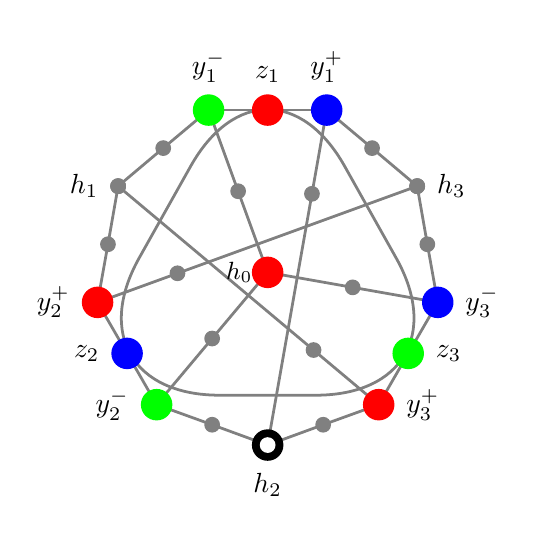
\begin{tikzpicture}  [scale=0.3]

\newdimen\ms
\ms=0.1cm

\tikzstyle{every path}=[line width=1pt]
\tikzstyle{c4}=[circle,inner sep={\ms/8},minimum size=4*\ms]
\tikzstyle{c3}=[circle,inner sep={\ms/8},minimum size=3*\ms]
\tikzstyle{c2}=[circle,inner sep={\ms/8},minimum size=2*\ms]
\tikzstyle{c1}=[circle,inner sep={\ms/8},minimum size=1.1*\ms]



		% Define positions of all observables
		\path
     (-2.50, 6.87    ) coordinate(2)     % $y_1^-
			  (-6.33,   3.65  ) coordinate(4)    % h_1
			  (-7.20, -1.27   ) coordinate(6)       % y_2^+
			  (-4.70, -5.60   ) coordinate(8)       % y_2^-
			  (0, -7.31       ) coordinate(10)       % h_2
			  (4.70, -5.60    ) coordinate(12)        % y_3^+$
     (7.20, -1.27    ) coordinate(14)       % y_3^-
			  (6.33, 3.65     ) coordinate(16)       % h_3
			  (2.50, 6.87     ) coordinate(18)    % y_1^+

			  (0, 6.87        ) coordinate(1)     % $z_1$
			  (-4.42, 5.26    ) coordinate(3)
			  (-6.76, 1.19    ) coordinate(5)
			  (-5.95, -3.43   ) coordinate(7)     % $z_2$
			  (-2.35, -6.45   ) coordinate(9)
     (2.35, -6.45    ) coordinate(11)
			  (5.95,-3.43     ) coordinate(13)    % $z_3$
			  (6.76, 1.19     ) coordinate(15)
		   (4.42, 5.26     ) coordinate(17)

     (0,0) coordinate(19)


(0, 10.3       ) coordinate(20)     % ze1
			  (-8.7, -5.2    ) coordinate(21)     % ze2
			  (8.7,-5.2    ) coordinate(22)    % ze3


     (-1.25, 3.435 ) coordinate(23)
     (3.60, -0.635 ) coordinate(24)
     (-2.35, -2.80 ) coordinate(25)
% h1={-6.33,   3.65  }; h3p={4.70, -5.60    } ; h1d2=  (h1+h3p )/2 ; c1=  (h1d2+h3p )/2
     (1.9425, -3.2875) coordinate(26)
% h2={0, -7.31    }; h1p={2.50, 6.87   } ; h2d2=  (h2+h1p )/2 ; c2=  (h2d2+h1p )/2
     (1.875, 3.325) coordinate(27)
% h3={6.33, 3.65    }; h2p={-7.20, -1.27    } ; h3d2=  (h3+h2p )/2 ; c3=  (h3d2+h2p )/2
     (-3.8175, -0.04) coordinate(28)
;

%(4.70-6.33,   3.65  -5.60   ) coordinate(4)    % h_1

	
		% Draw all the context curves
		
\draw [rounded corners=20mm,color=gray]     (20) -- (21) -- (22) --  cycle;


\draw [color=gray] (18) -- (1) -- (2);
\draw [color=gray] (2) -- (3) -- (4);
\draw [color=gray] (4) -- (5) -- (6);
\draw [color=gray] (6) -- (7) -- (8);
\draw [color=gray] (8) -- (9) -- (10);
\draw [color=gray] (10) -- (11) -- (12) ;

\draw [color=gray] (12) -- (13) -- (14);
\draw [color=gray] (14) -- (15) -- (16);
\draw [color=gray] (16) -- (17) -- (18);

\draw [color=gray] (19) -- (2);
\draw [color=gray] (19) -- (8);
\draw [color=gray] (19) -- (14);

\draw [color=gray] (4) -- (12);
\draw [color=gray] (10) -- (18);
\draw [color=gray] (16) -- (6);





%\draw [color=gray](0,0) circle (6.87);



\draw (19) coordinate[c4,fill=red,label={[xshift=4.5pt]180:{\small $h_0$}}];


\draw (1)  coordinate[c4,fill=red,label=90:$z_1$];

\draw (2)  coordinate[c4,fill=green,label=90:$y_1^-$];

\draw (3)  coordinate[c2,fill=gray];

\draw (4)  coordinate[c2,fill=gray,label=180:$h_1$];
\draw (4)  coordinate[c2,fill=gray];
\draw (4)  coordinate[c2,fill=gray];

\draw (5)  coordinate[c2,fill=gray,label=0:$ $];

\draw (6)  coordinate[c4,fill=red,label=180:$y_2^+$];

\draw (7)  coordinate[c4,fill=blue,label=180:$z_2$];

\draw (8)  coordinate[c4,fill=green,label=180:$y_2^-$];

\draw (9)  coordinate[c2,fill=gray,label=0:$ $];

\draw (10) coordinate[c4,fill=black,label=270:$h_2$];
\draw (10) coordinate[c2,fill=white];

\draw (11) coordinate[c2,fill=gray,label=0:$ $];

\draw (12) coordinate[c4,fill=red,label=0:$y_3^+$];

\draw (13) coordinate[c4,fill=green,label=0:$z_3$];

\draw (14) coordinate[c4,fill=blue,label=0:$y_3^-$];

\draw (15) coordinate[c2,fill=gray,label=0:$ $];

\draw (16) coordinate[c2,fill=gray,label=0:$h_3$];
\draw (16) coordinate[c2,fill=gray];
\draw (16) coordinate[c2,fill=gray];

\draw (17) coordinate[c2,fill=gray,label=0:$ $];

\draw (18) coordinate[c4,fill=blue,label=90:$y_1^+$];

\draw (23) coordinate[c2,fill=gray];
\draw (24) coordinate[c2,fill=gray];
\draw (25) coordinate[c2,fill=gray];
\draw (26) coordinate[c2,fill=gray];
\draw (27) coordinate[c2,fill=gray];
\draw (28) coordinate[c2,fill=gray];


		\end{tikzpicture}
&
\begin{tikzpicture}  [scale=0.4]
\newdimen\ms
\ms=0.1cm

\tikzstyle{every path}=[line width=1pt]
\tikzstyle{c4}=[circle,inner sep={\ms/8},minimum size=4*\ms]
\tikzstyle{c3}=[circle,inner sep={\ms/8},minimum size=3*\ms]
\tikzstyle{c2}=[circle,inner sep={\ms/8},minimum size=2*\ms]
\tikzstyle{c1}=[circle,inner sep={\ms/8},minimum size=1.1*\ms]

% Radius of regular polygons
\newdimen\R
\R=6cm
%\r= { \R * sqrt(3)/2}
\newdimen\K
\K=3cm

% Define positions of all observables
\path
  ({90 + 0 * 360 /5}:\R      ) coordinate(1)
  ({90 + 360 /10 + 0 * 360/5} : {\R * 0.6881/0.8507} ) coordinate(2)
  ({90 + 1 * 360 /5}:\R   ) coordinate(3)
  ({90 + 360 /10 + 1 * 360/5} : {\R * 0.6881/0.8507} ) coordinate(4)
  ({90 + 2 * 360 /5}:\R  ) coordinate(5)
  ({90 + 360 /10 + 2 * 360/5} : {\R * 0.6881/0.8507} ) coordinate(6)
  ({90 + 3 * 360 /5}:\R  ) coordinate(7)
  ({90 + 360 /10 + 3 * 360/5} : {\R * 0.6881/0.8507} ) coordinate(8)
  ({90 + 4 * 360 /5}:\R     ) coordinate(9)
  ({90 + 360 /10 + 4 * 360/5} : {\R * 0.6881/0.8507} ) coordinate(10)
  ({90 + 0 * 360 /5}:\K      ) coordinate(11)
  ({90 + 360 /10 + 0 * 360/5} : {\K * 0.6881/0.8507} ) coordinate(12)
  ({90 + 1 * 360 /5}:\K   ) coordinate(13)
  ({90 + 360 /10 + 1 * 360/5} : {\K * 0.6881/0.8507} ) coordinate(14)
  ({90 + 2 * 360 /5}:\K  ) coordinate(15)
  ({90 + 360 /10 + 2 * 360/5} : {\K * 0.6881/0.8507} ) coordinate(16)
  ({90 + 3 * 360 /5}:\K  ) coordinate(17)
  ({90 + 360 /10 + 3 * 360/5} : {\R * 0.6881/0.8507} ) coordinate(18)
  ({90 + 4 * 360 /5}:\K     ) coordinate(19)
  ({90 + 360 /10 + 4 * 360/5} : {\K * 0.6881/0.8507} ) coordinate(20)

  ({90 + 2 * 360 /5}:{(\R+\K)/2}) coordinate(21)

;

% draw contexts

\draw [color=gray] (1) -- (2) -- (3);
\draw [color=gray] (3) -- (4) -- (5);
\draw [color=gray] (5) -- (6) -- (7);
\draw [color=gray] (7) -- (8) -- (9);
\draw [color=gray] (9) -- (10) -- (1);    %

\draw [color=gray] (11) -- (15) ;
\draw [color=gray] (15) -- (19);
\draw [color=gray] (19) -- (13);
\draw [color=gray] (13) -- (17);
\draw [color=gray] (17) -- (11);

\draw ($ (11) !.5! (15) $) coordinate[c2,fill=gray];  %
\draw ($ (15) !.5! (19) $) coordinate[c2,fill=gray];  %
\draw ($ (19) !.47! (13) $) coordinate[c2,fill=gray];  %
\draw ($ (17) !.5! (11) $) coordinate[c2,fill=gray];  %

\draw [color=gray] (1) -- (11);
\draw [color=gray] (3) -- (13);
\draw [color=gray] (5) -- (15);
\draw [color=gray] (7) -- (17);
\draw [color=gray] (9) -- (19);

\draw ($ (1) !.5! (11) $) coordinate[c2,fill=gray];  %
\draw ($ (3) !.5! (13) $) coordinate[c2,fill=gray];  %
\draw ($ (7) !.5! (17) $) coordinate[c2,fill=gray];  %
\draw ($ (9) !.5! (19) $) coordinate[c2,fill=gray];  %

\draw [color=gray] (10)  to   [out=-140,in=100] ($ (13) !.5! (17) $)  to   [out=-90,in=0] (21);
%
%%
%% draw atoms
%%
%
\draw (1) coordinate[c4,fill=blue,label=90:$y_1^+$];  %
%
\draw (2) coordinate[c2,fill=gray];    %
%
\draw (3) coordinate[c2,fill=gray,label=180:$h_3$];   %
\draw (3) coordinate[c2,fill=gray]; %
\draw (3) coordinate[c2,fill=gray];  %
%
\draw (4) coordinate[c2,fill=gray];  %
%
\draw (5) coordinate[c4,fill=red,label=270:$y_2^+$];  %
%
\draw (6) coordinate[c2,fill=gray];
%
\draw (7) coordinate[c2,fill=gray,label=270:$h_1$];  %
\draw (7) coordinate[c2,fill=gray];  %
\draw (7) coordinate[c2,fill=gray];  %
%
\draw (8) coordinate[c2,fill=gray];  %
%
\draw (9) coordinate[c4,fill=green,label=0:$y_1^-$];
%
\draw (10) coordinate[c4,fill=red,label=0:$z_1$];  %
%
\draw (11) coordinate[c4,fill=black,label=180:$h_2$];  %
\draw (11) coordinate[c2,fill=white];
%
%
\draw (13) coordinate[c4,fill=blue,label=90:$y_3^-$]; %
%
\draw (15) coordinate[c4,fill=green,label=180:$y_2^-$]; %

\draw (17) coordinate[c4,fill=red,label=0:$y_3^+$];  %

\draw (19) coordinate[c4,fill=red,label=90:$h_0$]; %

%
\draw (21) coordinate[c4,fill=blue,label=-15:$z_2$];  %

\draw ($ (13) !.5! (17) $) coordinate[c4,fill=green,label=45:$z_3$];  %


\end{tikzpicture}
\\
(e)&(f)
\end{tabular}
\end{center}
\caption{\label{2025-b-f-Yu-2012-c1} (Color online)
Case 1 of the proof that the Yu-Oh hypergraph depicted in Figure~\ref{2017-b-f-Yu-2012} cannot be (noncontextually)
colored by three colors: its chromatic number is four.
}
\end{figure*}

%\newpage

\begin{figure*}
\begin{center}
\begin{tabular}{cc}
		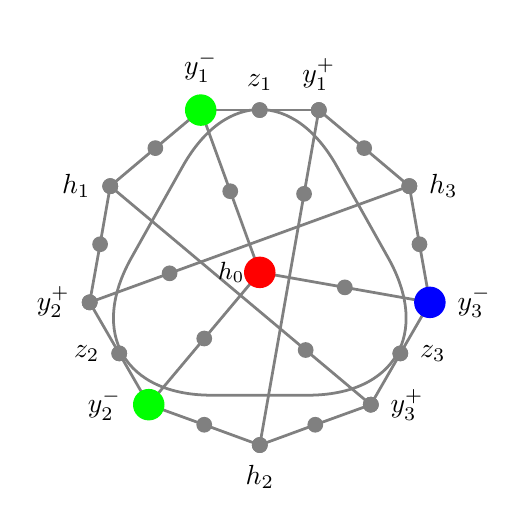
\begin{tikzpicture}  [scale=0.3]

\newdimen\ms
\ms=0.1cm

\tikzstyle{every path}=[line width=1pt]
\tikzstyle{c4}=[circle,inner sep={\ms/8},minimum size=4*\ms]
\tikzstyle{c3}=[circle,inner sep={\ms/8},minimum size=3*\ms]
\tikzstyle{c2}=[circle,inner sep={\ms/8},minimum size=2*\ms]
\tikzstyle{c1}=[circle,inner sep={\ms/8},minimum size=1.1*\ms]



		% Define positions of all observables
		\path
     (-2.50, 6.87    ) coordinate(2)     % $y_1^-
			  (-6.33,   3.65  ) coordinate(4)    % h_1
			  (-7.20, -1.27   ) coordinate(6)       % y_2^+
			  (-4.70, -5.60   ) coordinate(8)       % y_2^-
			  (0, -7.31       ) coordinate(10)       % h_2
			  (4.70, -5.60    ) coordinate(12)        % y_3^+$
     (7.20, -1.27    ) coordinate(14)       % y_3^-
			  (6.33, 3.65     ) coordinate(16)       % h_3
			  (2.50, 6.87     ) coordinate(18)    % y_1^+

			  (0, 6.87        ) coordinate(1)     % $z_1$
			  (-4.42, 5.26    ) coordinate(3)
			  (-6.76, 1.19    ) coordinate(5)
			  (-5.95, -3.43   ) coordinate(7)     % $z_2$
			  (-2.35, -6.45   ) coordinate(9)
     (2.35, -6.45    ) coordinate(11)
			  (5.95,-3.43     ) coordinate(13)    % $z_3$
			  (6.76, 1.19     ) coordinate(15)
		   (4.42, 5.26     ) coordinate(17)

     (0,0) coordinate(19)


(0, 10.3       ) coordinate(20)     % ze1
			  (-8.7, -5.2    ) coordinate(21)     % ze2
			  (8.7,-5.2    ) coordinate(22)    % ze3


     (-1.25, 3.435 ) coordinate(23)
     (3.60, -0.635 ) coordinate(24)
     (-2.35, -2.80 ) coordinate(25)
% h1={-6.33,   3.65  }; h3p={4.70, -5.60    } ; h1d2=  (h1+h3p )/2 ; c1=  (h1d2+h3p )/2
     (1.9425, -3.2875) coordinate(26)
% h2={0, -7.31    }; h1p={2.50, 6.87   } ; h2d2=  (h2+h1p )/2 ; c2=  (h2d2+h1p )/2
     (1.875, 3.325) coordinate(27)
% h3={6.33, 3.65    }; h2p={-7.20, -1.27    } ; h3d2=  (h3+h2p )/2 ; c3=  (h3d2+h2p )/2
     (-3.8175, -0.04) coordinate(28)
;

%(4.70-6.33,   3.65  -5.60   ) coordinate(4)    % h_1

	
		% Draw all the context curves
		
\draw [rounded corners=20mm,color=gray]     (20) -- (21) -- (22) --  cycle;


\draw [color=gray] (18) -- (1) -- (2);
\draw [color=gray] (2) -- (3) -- (4);
\draw [color=gray] (4) -- (5) -- (6);
\draw [color=gray] (6) -- (7) -- (8);
\draw [color=gray] (8) -- (9) -- (10);
\draw [color=gray] (10) -- (11) -- (12) ;

\draw [color=gray] (12) -- (13) -- (14);
\draw [color=gray] (14) -- (15) -- (16);
\draw [color=gray] (16) -- (17) -- (18);

\draw [color=gray] (19) -- (2);
\draw [color=gray] (19) -- (8);
\draw [color=gray] (19) -- (14);

\draw [color=gray] (4) -- (12);
\draw [color=gray] (10) -- (18);
\draw [color=gray] (16) -- (6);





%\draw [color=gray](0,0) circle (6.87);



\draw (19) coordinate[c4,fill=red,label={[xshift=4.5pt]180:{\small $h_0$}}];


\draw (1)  coordinate[c2,fill=gray,label=90:$z_1$];
\draw (1)  coordinate[c2,fill=gray];

\draw (2)  coordinate[c4,fill=green,label=90:$y_1^-$];

\draw (3)  coordinate[c2,fill=gray];

\draw (4)  coordinate[c2,fill=gray,label=180:$h_1$];
\draw (4)  coordinate[c2,fill=gray];
\draw (4)  coordinate[c2,fill=gray];

\draw (5)  coordinate[c2,fill=gray,label=0:$ $];

\draw (6)  coordinate[c2,fill=gray,fill=gray,label=180:$y_2^+$];
\draw (6)  coordinate[c2,fill=gray];
\draw (6)  coordinate[c2,fill=gray];

\draw (7)  coordinate[c2,fill=gray,label=180:$z_2$];
\draw (7)  coordinate[c2,fill=gray];

\draw (8)  coordinate[c4,fill=green,label=180:$y_2^-$];

\draw (9)  coordinate[c2,fill=gray,label=0:$ $];

\draw (10) coordinate[c2,fill=gray,label=270:$h_2$];
\draw (10) coordinate[c2,fill=gray];
\draw (10) coordinate[c2,fill=gray];

\draw (11) coordinate[c2,fill=gray,label=0:$ $];

\draw (12) coordinate[c2,fill=gray,label=0:$y_3^+$];
\draw (12) coordinate[c2,fill=gray];
\draw (12) coordinate[c2,fill=gray];

\draw (13) coordinate[c2,fill=gray,label=0:$z_3$];
\draw (13) coordinate[c2,fill=gray];

\draw (14) coordinate[c4,fill=blue,label=0:$y_3^-$];

\draw (15) coordinate[c2,fill=gray,label=0:$ $];

\draw (16) coordinate[c2,fill=gray,label=0:$h_3$];
\draw (16) coordinate[c2,fill=gray];
\draw (16) coordinate[c2,fill=gray];

\draw (17) coordinate[c2,fill=gray,label=0:$ $];

\draw (18) coordinate[c2,fill=gray,label=90:$y_1^+$];
\draw (18) coordinate[c2,fill=gray];
\draw (18) coordinate[c2,fill=gray];

\draw (23) coordinate[c2,fill=gray];
\draw (24) coordinate[c2,fill=gray];
\draw (25) coordinate[c2,fill=gray];
\draw (26) coordinate[c2,fill=gray];
\draw (27) coordinate[c2,fill=gray];
\draw (28) coordinate[c2,fill=gray];


		\end{tikzpicture}
&
\begin{tikzpicture}  [scale=0.4]
\newdimen\ms
\ms=0.1cm

\tikzstyle{every path}=[line width=1pt]
\tikzstyle{c4}=[circle,inner sep={\ms/8},minimum size=4*\ms]
\tikzstyle{c3}=[circle,inner sep={\ms/8},minimum size=3*\ms]
\tikzstyle{c2}=[circle,inner sep={\ms/8},minimum size=2*\ms]
\tikzstyle{c1}=[circle,inner sep={\ms/8},minimum size=1.1*\ms]

% Radius of regular polygons
\newdimen\R
\R=6cm
%\r= { \R * sqrt(3)/2}
\newdimen\K
\K=3cm

% Define positions of all observables
\path
  ({90 + 0 * 360 /5}:\R      ) coordinate(1)
  ({90 + 360 /10 + 0 * 360/5} : {\R * 0.6881/0.8507} ) coordinate(2)
  ({90 + 1 * 360 /5}:\R   ) coordinate(3)
  ({90 + 360 /10 + 1 * 360/5} : {\R * 0.6881/0.8507} ) coordinate(4)
  ({90 + 2 * 360 /5}:\R  ) coordinate(5)
  ({90 + 360 /10 + 2 * 360/5} : {\R * 0.6881/0.8507} ) coordinate(6)
  ({90 + 3 * 360 /5}:\R  ) coordinate(7)
  ({90 + 360 /10 + 3 * 360/5} : {\R * 0.6881/0.8507} ) coordinate(8)
  ({90 + 4 * 360 /5}:\R     ) coordinate(9)
  ({90 + 360 /10 + 4 * 360/5} : {\R * 0.6881/0.8507} ) coordinate(10)
  ({90 + 0 * 360 /5}:\K      ) coordinate(11)
  ({90 + 360 /10 + 0 * 360/5} : {\K * 0.6881/0.8507} ) coordinate(12)
  ({90 + 1 * 360 /5}:\K   ) coordinate(13)
  ({90 + 360 /10 + 1 * 360/5} : {\K * 0.6881/0.8507} ) coordinate(14)
  ({90 + 2 * 360 /5}:\K  ) coordinate(15)
  ({90 + 360 /10 + 2 * 360/5} : {\K * 0.6881/0.8507} ) coordinate(16)
  ({90 + 3 * 360 /5}:\K  ) coordinate(17)
  ({90 + 360 /10 + 3 * 360/5} : {\R * 0.6881/0.8507} ) coordinate(18)
  ({90 + 4 * 360 /5}:\K     ) coordinate(19)
  ({90 + 360 /10 + 4 * 360/5} : {\K * 0.6881/0.8507} ) coordinate(20)

  ({90 + 2 * 360 /5}:{(\R+\K)/2}) coordinate(21)

;

% draw contexts

\draw [color=gray] (1) -- (2) -- (3);
\draw [color=gray] (3) -- (4) -- (5);
\draw [color=gray] (5) -- (6) -- (7);
\draw [color=gray] (7) -- (8) -- (9);
\draw [color=gray] (9) -- (10) -- (1);    %

\draw [color=gray] (11) -- (15) ;
\draw [color=gray] (15) -- (19);
\draw [color=gray] (19) -- (13);
\draw [color=gray] (13) -- (17);
\draw [color=gray] (17) -- (11);

\draw ($ (11) !.5! (15) $) coordinate[c2,fill=gray];  %
\draw ($ (15) !.5! (19) $) coordinate[c2,fill=gray];  %
\draw ($ (19) !.47! (13) $) coordinate[c2,fill=gray];  %
\draw ($ (17) !.5! (11) $) coordinate[c2,fill=gray];  %

\draw [color=gray] (1) -- (11);
\draw [color=gray] (3) -- (13);
\draw [color=gray] (5) -- (15);
\draw [color=gray] (7) -- (17);
\draw [color=gray] (9) -- (19);

\draw ($ (1) !.5! (11) $) coordinate[c2,fill=gray];  %
\draw ($ (3) !.5! (13) $) coordinate[c2,fill=gray];  %
\draw ($ (7) !.5! (17) $) coordinate[c2,fill=gray];  %
\draw ($ (9) !.5! (19) $) coordinate[c2,fill=gray];  %

\draw [color=gray] (10)  to   [out=-140,in=100] ($ (13) !.5! (17) $)  to   [out=-90,in=0] (21);
%
%%
%% draw atoms
%%
%
\draw (1) coordinate[c2,fill=gray,label=90:$y_1^+$];  %
\draw (1) coordinate[c2,fill=gray];   %
\draw (1) coordinate[c2,fill=gray];  %
%
\draw (2) coordinate[c2,fill=gray];    %
%
\draw (3) coordinate[c2,fill=gray,label=180:$h_3$];   %
\draw (3) coordinate[c2,fill=gray]; %
\draw (3) coordinate[c2,fill=gray];  %
%
\draw (4) coordinate[c2,fill=gray];  %
%
\draw (5) coordinate[c2,fill=gray,label=270:$y_2^+$];  %
\draw (5) coordinate[c2,fill=gray];  %
\draw (5) coordinate[c2,fill=gray];  %
%
\draw (6) coordinate[c2,fill=gray];
%
\draw (7) coordinate[c2,fill=gray,label=270:$h_1$];  %
\draw (7) coordinate[c2,fill=gray];  %
\draw (7) coordinate[c2,fill=gray];  %
%
\draw (8) coordinate[c2,fill=gray];  %
%
\draw (9) coordinate[c4,fill=green,label=0:$y_1^-$];
%
\draw (10) coordinate[c2,fill=gray,label=0:$z_1$];  %
\draw (10) coordinate[c2,fill=gray];  %
%
\draw (11) coordinate[c2,fill=gray,label=180:$h_2$];  %
\draw (11) coordinate[c2,fill=gray];  %
\draw (11) coordinate[c2,fill=gray]; %
%
%
\draw (13) coordinate[c4,fill=blue,label=90:$y_3^-$]; %
%
\draw (15) coordinate[c4,fill=green,label=180:$y_2^-$]; %

\draw (17) coordinate[c2,fill=gray,label=0:$y_3^+$];  %
\draw (17) coordinate[c2,fill=gray];   %
\draw (17) coordinate[c2,fill=gray]; %

\draw (19) coordinate[c4,fill=red,label=90:$h_0$]; %

%
\draw (21) coordinate[c2,fill=gray];  %
\draw (21) coordinate[c2,fill=gray,label=-15:$z_2$];  %

\draw ($ (13) !.5! (17) $) coordinate[c2,fill=gray];  %
\draw ($ (13) !.5! (17) $) coordinate[c2,fill=gray,label=45:$z_3$];  %


\end{tikzpicture}
\\
(a)&(b)
\\
%$$$


%%%%%%%%%%%%%%%%%%%%%%%%%%%%%%%%%%%%%%%%%%%%%%%%%%%%%%%%%%%%%%%%%%%%%%%%%%%%%%%%%%%%%%%%%%%5
%%%%%%%%%%%%%%%%%%%%%%%%%%%%%%%%%%%%%%%%%%%%%%%%%%%%%%%%%%%%%%%%%%%%%%%%%%%%%%%%%%%%%%%%%%%5
%%%%%%%%%%%%%%%%%%%%%%%%%%%%%%%%%%%%%%%%%%%%%%%%%%%%%%%%%%%%%%%%%%%%%%%%%%%%%%%%%%%%%%%%%%%5
%%%%%%%%%%%%%%%%%%%%%%%%%%%%%%%%%%%%%%%%%%%%%%%%%%%%%%%%%%%%%%%%%%%%%%%%%%%%%%%%%%%%%%%%%%%5
%%%%%%%%%%%%%%%%%%%%%%%%%%%%%%%%%%%%%%%%%%%%%%%%%%%%%%%%%%%%%%%%%%%%%%%%%%%%%%%%%%%%%%%%%%%5
		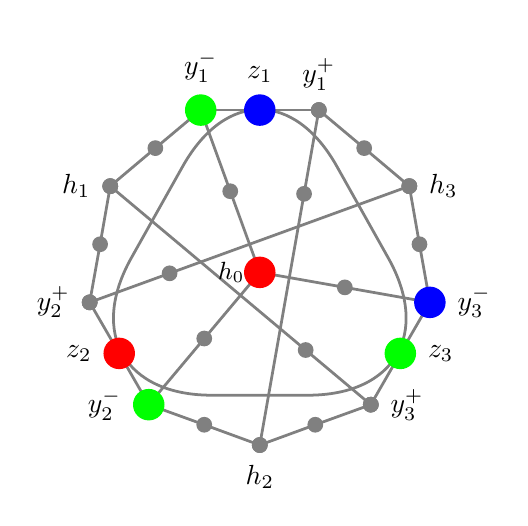
\begin{tikzpicture}  [scale=0.3]

\newdimen\ms
\ms=0.1cm

\tikzstyle{every path}=[line width=1pt]
\tikzstyle{c4}=[circle,inner sep={\ms/8},minimum size=4*\ms]
\tikzstyle{c3}=[circle,inner sep={\ms/8},minimum size=3*\ms]
\tikzstyle{c2}=[circle,inner sep={\ms/8},minimum size=2*\ms]
\tikzstyle{c1}=[circle,inner sep={\ms/8},minimum size=1.1*\ms]



		% Define positions of all observables
		\path
     (-2.50, 6.87    ) coordinate(2)     % $y_1^-
			  (-6.33,   3.65  ) coordinate(4)    % h_1
			  (-7.20, -1.27   ) coordinate(6)       % y_2^+
			  (-4.70, -5.60   ) coordinate(8)       % y_2^-
			  (0, -7.31       ) coordinate(10)       % h_2
			  (4.70, -5.60    ) coordinate(12)        % y_3^+$
     (7.20, -1.27    ) coordinate(14)       % y_3^-
			  (6.33, 3.65     ) coordinate(16)       % h_3
			  (2.50, 6.87     ) coordinate(18)    % y_1^+

			  (0, 6.87        ) coordinate(1)     % $z_1$
			  (-4.42, 5.26    ) coordinate(3)
			  (-6.76, 1.19    ) coordinate(5)
			  (-5.95, -3.43   ) coordinate(7)     % $z_2$
			  (-2.35, -6.45   ) coordinate(9)
     (2.35, -6.45    ) coordinate(11)
			  (5.95,-3.43     ) coordinate(13)    % $z_3$
			  (6.76, 1.19     ) coordinate(15)
		   (4.42, 5.26     ) coordinate(17)

     (0,0) coordinate(19)


(0, 10.3       ) coordinate(20)     % ze1
			  (-8.7, -5.2    ) coordinate(21)     % ze2
			  (8.7,-5.2    ) coordinate(22)    % ze3


     (-1.25, 3.435 ) coordinate(23)
     (3.60, -0.635 ) coordinate(24)
     (-2.35, -2.80 ) coordinate(25)
% h1={-6.33,   3.65  }; h3p={4.70, -5.60    } ; h1d2=  (h1+h3p )/2 ; c1=  (h1d2+h3p )/2
     (1.9425, -3.2875) coordinate(26)
% h2={0, -7.31    }; h1p={2.50, 6.87   } ; h2d2=  (h2+h1p )/2 ; c2=  (h2d2+h1p )/2
     (1.875, 3.325) coordinate(27)
% h3={6.33, 3.65    }; h2p={-7.20, -1.27    } ; h3d2=  (h3+h2p )/2 ; c3=  (h3d2+h2p )/2
     (-3.8175, -0.04) coordinate(28)
;

%(4.70-6.33,   3.65  -5.60   ) coordinate(4)    % h_1

	
		% Draw all the context curves
		
\draw [rounded corners=20mm,color=gray]     (20) -- (21) -- (22) --  cycle;


\draw [color=gray] (18) -- (1) -- (2);
\draw [color=gray] (2) -- (3) -- (4);
\draw [color=gray] (4) -- (5) -- (6);
\draw [color=gray] (6) -- (7) -- (8);
\draw [color=gray] (8) -- (9) -- (10);
\draw [color=gray] (10) -- (11) -- (12) ;

\draw [color=gray] (12) -- (13) -- (14);
\draw [color=gray] (14) -- (15) -- (16);
\draw [color=gray] (16) -- (17) -- (18);

\draw [color=gray] (19) -- (2);
\draw [color=gray] (19) -- (8);
\draw [color=gray] (19) -- (14);

\draw [color=gray] (4) -- (12);
\draw [color=gray] (10) -- (18);
\draw [color=gray] (16) -- (6);





%\draw [color=gray](0,0) circle (6.87);



\draw (19) coordinate[c4,fill=red,label={[xshift=4.5pt]180:{\small $h_0$}}];


\draw (1)  coordinate[c4,fill=blue,label=90:$z_1$];

\draw (2)  coordinate[c4,fill=green,label=90:$y_1^-$];

\draw (3)  coordinate[c2,fill=gray];

\draw (4)  coordinate[c2,fill=gray,label=180:$h_1$];
\draw (4)  coordinate[c2,fill=gray];
\draw (4)  coordinate[c2,fill=gray];

\draw (5)  coordinate[c2,fill=gray,label=0:$ $];

\draw (6)  coordinate[c2,fill=gray,fill=gray,label=180:$y_2^+$];
\draw (6)  coordinate[c2,fill=gray];
\draw (6)  coordinate[c2,fill=gray];

\draw (7)  coordinate[c4,fill=red,label=180:$z_2$];

\draw (8)  coordinate[c4,fill=green,label=180:$y_2^-$];

\draw (9)  coordinate[c2,fill=gray,label=0:$ $];

\draw (10) coordinate[c2,fill=gray,label=270:$h_2$];
\draw (10) coordinate[c2,fill=gray];
\draw (10) coordinate[c2,fill=gray];

\draw (11) coordinate[c2,fill=gray,label=0:$ $];

\draw (12) coordinate[c2,fill=gray,label=0:$y_3^+$];
\draw (12) coordinate[c2,fill=gray];
\draw (12) coordinate[c2,fill=gray];

\draw (13) coordinate[c4,fill=green,label=0:$z_3$];

\draw (14) coordinate[c4,fill=blue,label=0:$y_3^-$];

\draw (15) coordinate[c2,fill=gray,label=0:$ $];

\draw (16) coordinate[c2,fill=gray,label=0:$h_3$];
\draw (16) coordinate[c2,fill=gray];
\draw (16) coordinate[c2,fill=gray];

\draw (17) coordinate[c2,fill=gray,label=0:$ $];

\draw (18) coordinate[c2,fill=gray,label=90:$y_1^+$];
\draw (18) coordinate[c2,fill=gray];
\draw (18) coordinate[c2,fill=gray];

\draw (23) coordinate[c2,fill=gray];
\draw (24) coordinate[c2,fill=gray];
\draw (25) coordinate[c2,fill=gray];
\draw (26) coordinate[c2,fill=gray];
\draw (27) coordinate[c2,fill=gray];
\draw (28) coordinate[c2,fill=gray];


		\end{tikzpicture}
&
\begin{tikzpicture}  [scale=0.4]
\newdimen\ms
\ms=0.1cm

\tikzstyle{every path}=[line width=1pt]
\tikzstyle{c4}=[circle,inner sep={\ms/8},minimum size=4*\ms]
\tikzstyle{c3}=[circle,inner sep={\ms/8},minimum size=3*\ms]
\tikzstyle{c2}=[circle,inner sep={\ms/8},minimum size=2*\ms]
\tikzstyle{c1}=[circle,inner sep={\ms/8},minimum size=1.1*\ms]

% Radius of regular polygons
\newdimen\R
\R=6cm
%\r= { \R * sqrt(3)/2}
\newdimen\K
\K=3cm

% Define positions of all observables
\path
  ({90 + 0 * 360 /5}:\R      ) coordinate(1)
  ({90 + 360 /10 + 0 * 360/5} : {\R * 0.6881/0.8507} ) coordinate(2)
  ({90 + 1 * 360 /5}:\R   ) coordinate(3)
  ({90 + 360 /10 + 1 * 360/5} : {\R * 0.6881/0.8507} ) coordinate(4)
  ({90 + 2 * 360 /5}:\R  ) coordinate(5)
  ({90 + 360 /10 + 2 * 360/5} : {\R * 0.6881/0.8507} ) coordinate(6)
  ({90 + 3 * 360 /5}:\R  ) coordinate(7)
  ({90 + 360 /10 + 3 * 360/5} : {\R * 0.6881/0.8507} ) coordinate(8)
  ({90 + 4 * 360 /5}:\R     ) coordinate(9)
  ({90 + 360 /10 + 4 * 360/5} : {\R * 0.6881/0.8507} ) coordinate(10)
  ({90 + 0 * 360 /5}:\K      ) coordinate(11)
  ({90 + 360 /10 + 0 * 360/5} : {\K * 0.6881/0.8507} ) coordinate(12)
  ({90 + 1 * 360 /5}:\K   ) coordinate(13)
  ({90 + 360 /10 + 1 * 360/5} : {\K * 0.6881/0.8507} ) coordinate(14)
  ({90 + 2 * 360 /5}:\K  ) coordinate(15)
  ({90 + 360 /10 + 2 * 360/5} : {\K * 0.6881/0.8507} ) coordinate(16)
  ({90 + 3 * 360 /5}:\K  ) coordinate(17)
  ({90 + 360 /10 + 3 * 360/5} : {\R * 0.6881/0.8507} ) coordinate(18)
  ({90 + 4 * 360 /5}:\K     ) coordinate(19)
  ({90 + 360 /10 + 4 * 360/5} : {\K * 0.6881/0.8507} ) coordinate(20)

  ({90 + 2 * 360 /5}:{(\R+\K)/2}) coordinate(21)

;

% draw contexts

\draw [color=gray] (1) -- (2) -- (3);
\draw [color=gray] (3) -- (4) -- (5);
\draw [color=gray] (5) -- (6) -- (7);
\draw [color=gray] (7) -- (8) -- (9);
\draw [color=gray] (9) -- (10) -- (1);    %

\draw [color=gray] (11) -- (15) ;
\draw [color=gray] (15) -- (19);
\draw [color=gray] (19) -- (13);
\draw [color=gray] (13) -- (17);
\draw [color=gray] (17) -- (11);

\draw ($ (11) !.5! (15) $) coordinate[c2,fill=gray];  %
\draw ($ (15) !.5! (19) $) coordinate[c2,fill=gray];  %
\draw ($ (19) !.47! (13) $) coordinate[c2,fill=gray];  %
\draw ($ (17) !.5! (11) $) coordinate[c2,fill=gray];  %

\draw [color=gray] (1) -- (11);
\draw [color=gray] (3) -- (13);
\draw [color=gray] (5) -- (15);
\draw [color=gray] (7) -- (17);
\draw [color=gray] (9) -- (19);

\draw ($ (1) !.5! (11) $) coordinate[c2,fill=gray];  %
\draw ($ (3) !.5! (13) $) coordinate[c2,fill=gray];  %
\draw ($ (7) !.5! (17) $) coordinate[c2,fill=gray];  %
\draw ($ (9) !.5! (19) $) coordinate[c2,fill=gray];  %

\draw [color=gray] (10)  to   [out=-140,in=100] ($ (13) !.5! (17) $)  to   [out=-90,in=0] (21);
%
%%
%% draw atoms
%%
%
\draw (1) coordinate[c2,fill=gray,label=90:$y_1^+$];  %
\draw (1) coordinate[c2,fill=gray];   %
\draw (1) coordinate[c2,fill=gray];  %
%
\draw (2) coordinate[c2,fill=gray];    %
%
\draw (3) coordinate[c2,fill=gray,label=180:$h_3$];   %
\draw (3) coordinate[c2,fill=gray]; %
\draw (3) coordinate[c2,fill=gray];  %
%
\draw (4) coordinate[c2,fill=gray];  %
%
\draw (5) coordinate[c2,fill=gray,label=270:$y_2^+$];  %
\draw (5) coordinate[c2,fill=gray];  %
\draw (5) coordinate[c2,fill=gray];  %
%
\draw (6) coordinate[c2,fill=gray];
%
\draw (7) coordinate[c2,fill=gray,label=270:$h_1$];  %
\draw (7) coordinate[c2,fill=gray];  %
\draw (7) coordinate[c2,fill=gray];  %
%
\draw (8) coordinate[c2,fill=gray];  %
%
\draw (9) coordinate[c4,fill=green,label=0:$y_1^-$];
%
\draw (10) coordinate[c4,fill=blue,label=0:$z_1$];  %
%
\draw (11) coordinate[c2,fill=gray,label=180:$h_2$];  %
\draw (11) coordinate[c2,fill=gray];  %
\draw (11) coordinate[c2,fill=gray]; %
%
%
\draw (13) coordinate[c4,fill=blue,label=90:$y_3^-$]; %
%
\draw (15) coordinate[c4,fill=green,label=180:$y_2^-$]; %

\draw (17) coordinate[c2,fill=gray,label=0:$y_3^+$];  %
\draw (17) coordinate[c2,fill=gray];   %
\draw (17) coordinate[c2,fill=gray]; %

\draw (19) coordinate[c4,fill=red,label=90:$h_0$]; %

%
\draw (21) coordinate[c4,fill=red,label=-15:$z_2$];  %

\draw ($ (13) !.5! (17) $) coordinate[c4,fill=green,label=45:$z_3$];  %


\end{tikzpicture}
\\
(c)&(d)
\\
%%%%%%%%%%%%%%%%%%%%%%%%%%%%%%%%%%%%%%%%%%%%%%%%%%%%%%%%%%%%%%%%%%%%%%%%%%%%%%%%%%%%%%%%%%%5
%%%%%%%%%%%%%%%%%%%%%%%%%%%%%%%%%%%%%%%%%%%%%%%%%%%%%%%%%%%%%%%%%%%%%%%%%%%%%%%%%%%%%%%%%%%5
%%%%%%%%%%%%%%%%%%%%%%%%%%%%%%%%%%%%%%%%%%%%%%%%%%%%%%%%%%%%%%%%%%%%%%%%%%%%%%%%%%%%%%%%%%%5
%%%%%%%%%%%%%%%%%%%%%%%%%%%%%%%%%%%%%%%%%%%%%%%%%%%%%%%%%%%%%%%%%%%%%%%%%%%%%%%%%%%%%%%%%%%5
%%%%%%%%%%%%%%%%%%%%%%%%%%%%%%%%%%%%%%%%%%%%%%%%%%%%%%%%%%%%%%%%%%%%%%%%%%%%%%%%%%%%%%%%%%%5
		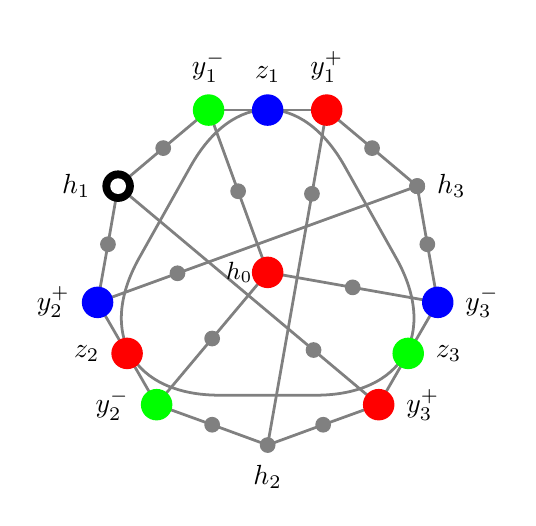
\begin{tikzpicture}  [scale=0.3]

\newdimen\ms
\ms=0.1cm

\tikzstyle{every path}=[line width=1pt]
\tikzstyle{c4}=[circle,inner sep={\ms/8},minimum size=4*\ms]
\tikzstyle{c3}=[circle,inner sep={\ms/8},minimum size=3*\ms]
\tikzstyle{c2}=[circle,inner sep={\ms/8},minimum size=2*\ms]
\tikzstyle{c1}=[circle,inner sep={\ms/8},minimum size=1.1*\ms]



		% Define positions of all observables
		\path
     (-2.50, 6.87    ) coordinate(2)     % $y_1^-
			  (-6.33,   3.65  ) coordinate(4)    % h_1
			  (-7.20, -1.27   ) coordinate(6)       % y_2^+
			  (-4.70, -5.60   ) coordinate(8)       % y_2^-
			  (0, -7.31       ) coordinate(10)       % h_2
			  (4.70, -5.60    ) coordinate(12)        % y_3^+$
     (7.20, -1.27    ) coordinate(14)       % y_3^-
			  (6.33, 3.65     ) coordinate(16)       % h_3
			  (2.50, 6.87     ) coordinate(18)    % y_1^+

			  (0, 6.87        ) coordinate(1)     % $z_1$
			  (-4.42, 5.26    ) coordinate(3)
			  (-6.76, 1.19    ) coordinate(5)
			  (-5.95, -3.43   ) coordinate(7)     % $z_2$
			  (-2.35, -6.45   ) coordinate(9)
     (2.35, -6.45    ) coordinate(11)
			  (5.95,-3.43     ) coordinate(13)    % $z_3$
			  (6.76, 1.19     ) coordinate(15)
		   (4.42, 5.26     ) coordinate(17)

     (0,0) coordinate(19)


(0, 10.3       ) coordinate(20)     % ze1
			  (-8.7, -5.2    ) coordinate(21)     % ze2
			  (8.7,-5.2    ) coordinate(22)    % ze3


     (-1.25, 3.435 ) coordinate(23)
     (3.60, -0.635 ) coordinate(24)
     (-2.35, -2.80 ) coordinate(25)
% h1={-6.33,   3.65  }; h3p={4.70, -5.60    } ; h1d2=  (h1+h3p )/2 ; c1=  (h1d2+h3p )/2
     (1.9425, -3.2875) coordinate(26)
% h2={0, -7.31    }; h1p={2.50, 6.87   } ; h2d2=  (h2+h1p )/2 ; c2=  (h2d2+h1p )/2
     (1.875, 3.325) coordinate(27)
% h3={6.33, 3.65    }; h2p={-7.20, -1.27    } ; h3d2=  (h3+h2p )/2 ; c3=  (h3d2+h2p )/2
     (-3.8175, -0.04) coordinate(28)
;

%(4.70-6.33,   3.65  -5.60   ) coordinate(4)    % h_1

	
		% Draw all the context curves
		
\draw [rounded corners=20mm,color=gray]     (20) -- (21) -- (22) --  cycle;


\draw [color=gray] (18) -- (1) -- (2);
\draw [color=gray] (2) -- (3) -- (4);
\draw [color=gray] (4) -- (5) -- (6);
\draw [color=gray] (6) -- (7) -- (8);
\draw [color=gray] (8) -- (9) -- (10);
\draw [color=gray] (10) -- (11) -- (12) ;

\draw [color=gray] (12) -- (13) -- (14);
\draw [color=gray] (14) -- (15) -- (16);
\draw [color=gray] (16) -- (17) -- (18);

\draw [color=gray] (19) -- (2);
\draw [color=gray] (19) -- (8);
\draw [color=gray] (19) -- (14);

\draw [color=gray] (4) -- (12);
\draw [color=gray] (10) -- (18);
\draw [color=gray] (16) -- (6);





%\draw [color=gray](0,0) circle (6.87);



\draw (19) coordinate[c4,fill=red,label={[xshift=4.5pt]180:{\small $h_0$}}];


\draw (1)  coordinate[c4,fill=blue,label=90:$z_1$];

\draw (2)  coordinate[c4,fill=green,label=90:$y_1^-$];

\draw (3)  coordinate[c2,fill=gray];

\draw (4)  coordinate[c4,fill=black,label=180:$h_1$];
\draw (4) coordinate[c2,fill=white];

\draw (5)  coordinate[c2,fill=gray,label=0:$ $];

\draw (6)  coordinate[c4,fill=blue,label=180:$y_2^+$];

\draw (7)  coordinate[c4,fill=red,label=180:$z_2$];

\draw (8)  coordinate[c4,fill=green,label=180:$y_2^-$];

\draw (9)  coordinate[c2,fill=gray,label=0:$ $];

\draw (10) coordinate[c2,fill=gray,label=270:$h_2$];


\draw (11) coordinate[c2,fill=gray,label=0:$ $];

\draw (12) coordinate[c4,fill=red,label=0:$y_3^+$];

\draw (13) coordinate[c4,fill=green,label=0:$z_3$];

\draw (14) coordinate[c4,fill=blue,label=0:$y_3^-$];

\draw (15) coordinate[c2,fill=gray,label=0:$ $];

\draw (16) coordinate[c2,fill=gray,label=0:$h_3$];
\draw (16) coordinate[c2,fill=gray];
\draw (16) coordinate[c2,fill=gray];

\draw (17) coordinate[c2,fill=gray,label=0:$ $];

\draw (18) coordinate[c4,fill=red,label=90:$y_1^+$];

\draw (23) coordinate[c2,fill=gray];
\draw (24) coordinate[c2,fill=gray];
\draw (25) coordinate[c2,fill=gray];
\draw (26) coordinate[c2,fill=gray];
\draw (27) coordinate[c2,fill=gray];
\draw (28) coordinate[c2,fill=gray];


		\end{tikzpicture}
&
\begin{tikzpicture}  [scale=0.4]
\newdimen\ms
\ms=0.1cm

\tikzstyle{every path}=[line width=1pt]
\tikzstyle{c4}=[circle,inner sep={\ms/8},minimum size=4*\ms]
\tikzstyle{c3}=[circle,inner sep={\ms/8},minimum size=3*\ms]
\tikzstyle{c2}=[circle,inner sep={\ms/8},minimum size=2*\ms]
\tikzstyle{c1}=[circle,inner sep={\ms/8},minimum size=1.1*\ms]

% Radius of regular polygons
\newdimen\R
\R=6cm
%\r= { \R * sqrt(3)/2}
\newdimen\K
\K=3cm

% Define positions of all observables
\path
  ({90 + 0 * 360 /5}:\R      ) coordinate(1)
  ({90 + 360 /10 + 0 * 360/5} : {\R * 0.6881/0.8507} ) coordinate(2)
  ({90 + 1 * 360 /5}:\R   ) coordinate(3)
  ({90 + 360 /10 + 1 * 360/5} : {\R * 0.6881/0.8507} ) coordinate(4)
  ({90 + 2 * 360 /5}:\R  ) coordinate(5)
  ({90 + 360 /10 + 2 * 360/5} : {\R * 0.6881/0.8507} ) coordinate(6)
  ({90 + 3 * 360 /5}:\R  ) coordinate(7)
  ({90 + 360 /10 + 3 * 360/5} : {\R * 0.6881/0.8507} ) coordinate(8)
  ({90 + 4 * 360 /5}:\R     ) coordinate(9)
  ({90 + 360 /10 + 4 * 360/5} : {\R * 0.6881/0.8507} ) coordinate(10)
  ({90 + 0 * 360 /5}:\K      ) coordinate(11)
  ({90 + 360 /10 + 0 * 360/5} : {\K * 0.6881/0.8507} ) coordinate(12)
  ({90 + 1 * 360 /5}:\K   ) coordinate(13)
  ({90 + 360 /10 + 1 * 360/5} : {\K * 0.6881/0.8507} ) coordinate(14)
  ({90 + 2 * 360 /5}:\K  ) coordinate(15)
  ({90 + 360 /10 + 2 * 360/5} : {\K * 0.6881/0.8507} ) coordinate(16)
  ({90 + 3 * 360 /5}:\K  ) coordinate(17)
  ({90 + 360 /10 + 3 * 360/5} : {\R * 0.6881/0.8507} ) coordinate(18)
  ({90 + 4 * 360 /5}:\K     ) coordinate(19)
  ({90 + 360 /10 + 4 * 360/5} : {\K * 0.6881/0.8507} ) coordinate(20)

  ({90 + 2 * 360 /5}:{(\R+\K)/2}) coordinate(21)

;

% draw contexts

\draw [color=gray] (1) -- (2) -- (3);
\draw [color=gray] (3) -- (4) -- (5);
\draw [color=gray] (5) -- (6) -- (7);
\draw [color=gray] (7) -- (8) -- (9);
\draw [color=gray] (9) -- (10) -- (1);    %

\draw [color=gray] (11) -- (15) ;
\draw [color=gray] (15) -- (19);
\draw [color=gray] (19) -- (13);
\draw [color=gray] (13) -- (17);
\draw [color=gray] (17) -- (11);

\draw ($ (11) !.5! (15) $) coordinate[c2,fill=gray];  %
\draw ($ (15) !.5! (19) $) coordinate[c2,fill=gray];  %
\draw ($ (19) !.47! (13) $) coordinate[c2,fill=gray];  %
\draw ($ (17) !.5! (11) $) coordinate[c2,fill=gray];  %

\draw [color=gray] (1) -- (11);
\draw [color=gray] (3) -- (13);
\draw [color=gray] (5) -- (15);
\draw [color=gray] (7) -- (17);
\draw [color=gray] (9) -- (19);

\draw ($ (1) !.5! (11) $) coordinate[c2,fill=gray];  %
\draw ($ (3) !.5! (13) $) coordinate[c2,fill=gray];  %
\draw ($ (7) !.5! (17) $) coordinate[c2,fill=gray];  %
\draw ($ (9) !.5! (19) $) coordinate[c2,fill=gray];  %

\draw [color=gray] (10)  to   [out=-140,in=100] ($ (13) !.5! (17) $)  to   [out=-90,in=0] (21);
%
%%
%% draw atoms
%%
%
\draw (1) coordinate[c4,fill=red,label=90:$y_1^+$];  %
%
\draw (2) coordinate[c2,fill=gray];    %
%
\draw (3) coordinate[c2,fill=gray,label=180:$h_3$];   %
\draw (3) coordinate[c2,fill=gray]; %
\draw (3) coordinate[c2,fill=gray];  %
%
\draw (4) coordinate[c2,fill=gray];  %
%
\draw (5) coordinate[c4,fill=blue,label=270:$y_2^+$];  %
%
\draw (6) coordinate[c2,fill=gray];
%
\draw (7) coordinate[c4,fill=black,label=270:$h_1$];  %
\draw (7) coordinate[c2,fill=white];
%
\draw (8) coordinate[c2,fill=gray];  %
%
\draw (9) coordinate[c4,fill=green,label=0:$y_1^-$];
%
\draw (10) coordinate[c4,fill=blue,label=0:$z_1$];  %
%
\draw (11) coordinate[c2,fill=gray,label=180:$h_2$];  %
;
%
%
\draw (13) coordinate[c4,fill=blue,label=90:$y_3^-$]; %
%
\draw (15) coordinate[c4,fill=green,label=180:$y_2^-$]; %

\draw (17) coordinate[c4,fill=red,label=0:$y_3^+$];  %

\draw (19) coordinate[c4,fill=red,label=90:$h_0$]; %

%
\draw (21) coordinate[c4,fill=red,label=-15:$z_2$];  %

\draw ($ (13) !.5! (17) $) coordinate[c4,fill=green,label=45:$z_3$];  %


\end{tikzpicture}
\\
(e)&(f)
\end{tabular}
\end{center}
\caption{\label{2025-b-f-Yu-2012-c2} (Color online)
Case 2 of the proof that the Yu-Oh hypergraph depicted in Figure~\ref{2017-b-f-Yu-2012} cannot be (noncontextually)
colored by three colors: its chromatic number is four.
}
\end{figure*}

\section{Summary}

Chromatic contextuality, characterized by the impossibility of admissibly coloring an $n$-uniform hypergraph with $n$ colors per hyperedge,
presents a compelling case against the existence of classical (noncontextual) hidden parameters.
In this way, chromatic contextuality resembles Kochen-Specker contextuality,
which is defined by the absence of uniform two-valued states~\cite{kochen1,Cabello-1996ega},
or admissible states~\cite{2015-AnalyticKS}.
Chromatic contextuality can be viewed as an extreme form of operator-valued argument,
given that the number of values involved is equivalent to the number of vertices in each context-edge of the hypergraph.

Chromatic contextuality, in contrast to Kochen-Specker contextuality, constitutes a distinct criterion for nonclassicality:
The respective hypergraphs and the collection of quantum observables they represent
may still support two-valued states and even permit (though not necessarily imply) classical embeddability
through a separating set of two-valued states.
This is exemplified by Greechie's \( G_{32} \) hypergraph,
which admits a set representation in terms of a partition logic~\cite[Appendix~B, p.~032104-16f]{svozil-2021-chroma}.


Moreover, any \( n \)-coloring can be directly converted into a two-valued state---indeed, into \( n \) two-valued states---by
aggregation, that is, by
reducing or folding the number of \( n \) colors into two.
This can be done by identifying a single color with the value \( 1 \) and all remaining colors with \( 0 \).
In this way, the set of observables encoding the hypergraph is equi-partitioned.



Alternatively, an \( n \)-coloring can be used by identifying more than one color with a non-zero value~\cite{ramanathan-2024},
for example, identifying two colors with the value \( 1/2 \).
A single coloring thus defines a canonical set of \( n \) two-valued states
covering the entire hypergraph~\cite[Appendix~A]{svozil-2021-chroma}.

However, the converse is not true: The existence of even separating sets of two-valued states does not imply the existence of a coloring,
as demonstrated by the aforementioned example of $G_{32}$.

It is quite remarkable that not all such colorings can be derived from the nonexclusive hypergraph coloring scheme discussed above.
In particular, the exotic two-times-\( 1/2 \) coloring of the pentagon (or house or pentagram) on intertwining context-hyperedges,
as exposed by Greechie~\cite[Figure~5, p.~186]{greechie-1974} and Wright~\cite[$\omega_{0}$, p.~268]{wright:pent},
cannot be obtained through identifying colors. The reason for this is a parity argument:
For an odd number of hyperedges, such as five, there cannot exist a coloring with the same color assigned to all (odd-numbered)
intertwining vertices.


By the same parity reasoning, one of the eleven two-valued states of the pentagon,
in which all the values are assigned to the nonintertwining `middle' vertices, does not originate from the aggregation
from a hypergraph coloring. Suppose one of the colors, say red, is always centered in the middle;
this would imply that the other two colors, say green and blue, must alternate at the five vertices with intertwining contexts.
However, for an odd number of such intertwining vertices, this leads to a disallowed configuration;
more explicitly, to green-red-blue-red-green-red-blue-red-\textit{green-red-green} (from cycle).
If this two-valued state is eliminated, the Hull computation still yields Klyachko's pentagram inequality~\cite[Equation~(5)]{Klyachko-2008},
along with an additional upper bound:
$1 \ge A_{13}+A_{35}+A_{57}+A_{79}+A_{91}\ge - 3$.
This explicit house-pentagon-pentagram example also demonstrates that, for hyperedges with more than two vertices,
not all two-valued states can necessarily be derived by aggregation---the
irreversible mapping of one color to the value $1$ and all other colors to $0$.
The Bub and Stairs inequality~\cite{Bub-2009} remains unaffected as they do not use the `color-fobidden middle-center' two-valued state.
This topic is too broad to be fully addressed within the scope of this paper.

For physical reasons we suggest that every two-valued state should ultimately originate from `perfect',
that is, maximal, measurements corresponding to colorings.
Therefore, only two-valued states that are derived through aggregation should be considered when deriving,
for instance, Boole-Bell-type inequalities by solving the Hull problem for the respective correlation polytope~\cite{froissart-81,pitowsky-86}.
Two-valued states that cannot be represented by aggregation from colorings are unphysical in the sense that no
(classical) maximal observables or contexts exist that could justify their inclusion.

The chromatic analogue of True-Implies-False (TIFs) and True-Implies-True (TITs) gadgets~\cite{2018-minimalYIYS}, which exhibit a distinct form of contextuality,
such as Hardy-type~\cite{svozil-2020-hardy}, has not yet been explored in the context of hypergraph colorings.
Additionally, the concept of chromatic separability, similar to Kochen-Specker's demarcation criterion of (non)separability with respect to two-valued states, remains to be discussed.
For instance, does nonseparability by two-valued states imply chromatic nonseparability?
We note that Kochen and Specker's $\Gamma_3$~\cite{kochen1} is also color nonseparable.
Is aggregation sufficient  for the inheritance of such properties?
These topics require future investigation.




%%%%%%%%%%%%%%%%%%%%%%%%%%%%%%%%%%%%%%%%%%%%%%%%%%%%%%%%%%%%%%%%%%%%%%%%%%%%%%%%%%%%%%%%%%%%%%%%%%%%%%%%%%%%%%%%%%%%%%%%%%%%%%%%%%%%
\ifws
%%%%%%%%%%%%%%%%%%%%%%%%%%%%%%%%%%%%%%%%%%
\vspace{6pt}

%%%%%%%%%%%%%%%%%%%%%%%%%%%%%%%%%%%%%%%%%%
%% optional
%\supplementary{The following supporting information can be downloaded at:  \linksupplementary{s1}, Figure S1: title; Table S1: title; Video S1: title.}

% Only for journal Methods and Protocols:
% If you wish to submit a video article, please do so with any other supplementary material.
% \supplementary{The following supporting information can be downloaded at: \linksupplementary{s1}, Figure S1: title; Table S1: title; Video S1: title. A supporting video article is available at doi: link.}

% Only used for preprtints:
% \supplementary{The following supporting information can be downloaded at the website of this paper posted on \href{https://www.preprints.org/}{Preprints.org}.}

% Only for journal Hardware:
% If you wish to submit a video article, please do so with any other supplementary material.
% \supplementary{The following supporting information can be downloaded at: \linksupplementary{s1}, Figure S1: title; Table S1: title; Video S1: title.\vspace{6pt}\\
%\begin{tabularx}{\textwidth}{lll}
%\toprule
%\textbf{Name} & \textbf{Type} & \textbf{Description} \\
%\midrule
%S1 & Python script (.py) & Script of python source code used in XX \\
%S2 & Text (.txt) & Script of modelling code used to make Figure X \\
%S3 & Text (.txt) & Raw data from experiment X \\
%S4 & Video (.mp4) & Video demonstrating the hardware in use \\
%... & ... & ... \\
%\bottomrule
%\end{tabularx}
%}

%%%%%%%%%%%%%%%%%%%%%%%%%%%%%%%%%%%%%%%%%%
%\authorcontributions{For research articles with several authors, a short paragraph specifying their individual contributions must be provided. The following statements should be used ``Conceptualization, X.X. and Y.Y.; methodology, X.X.; software, X.X.; validation, X.X., Y.Y. and Z.Z.; formal analysis, X.X.; investigation, X.X.; resources, X.X.; data curation, X.X.; writing---original draft preparation, X.X.; writing---review and editing, X.X.; visualization, X.X.; supervision, X.X.; project administration, X.X.; funding acquisition, Y.Y. All authors have read and agreed to the published version of the manuscript.'', please turn to the  \href{http://img.mdpi.org/data/contributor-role-instruction.pdf}{CRediT taxonomy} for the term explanation. Authorship must be limited to those who have contributed substantially to the work~reported.}

\funding{
This research was funded in whole or in part by the Austrian Science Fund (FWF) [Grant DOI:10.55776/I4579].
%The author acknowledges TU Wien Bibliothek for financial support through its Open Access Funding Programme.
}

%\institutionalreview{In this section, you should add the Institutional Review Board Statement and approval number, if relevant to your study. You might choose to exclude this statement if the study did not require ethical approval. Please note that the Editorial Office might ask you for further information. Please add “The study was conducted in accordance with the Declaration of Helsinki, and approved by the Institutional Review Board (or Ethics Committee) of NAME OF INSTITUTE (protocol code XXX and date of approval).” for studies involving humans. OR “The animal study protocol was approved by the Institutional Review Board (or Ethics Committee) of NAME OF INSTITUTE (protocol code XXX and date of approval).” for studies involving animals. OR “Ethical review and approval were waived for this study due to REASON (please provide a detailed justification).” OR “Not applicable” for studies not involving humans or animals.}

%\informedconsent{Any research article describing a study involving humans should contain this statement. Please add ``Informed consent was obtained from all subjects involved in the study.'' OR ``Patient consent was waived due to REASON (please provide a detailed justification).'' OR ``Not applicable'' for studies not involving humans. You might also choose to exclude this statement if the study did not involve humans.

%Written informed consent for publication must be obtained from participating patients who can be identified (including by the patients themselves). Please state ``Written informed consent has been obtained from the patient(s) to publish this paper'' if applicable.}

%\dataavailability{We encourage all authors of articles published in MDPI journals to share their research data. In this section, please provide details regarding where data supporting reported results can be found, including links to publicly archived datasets analyzed or generated during the study. Where no new data were created, or where data is unavailable due to privacy or ethical restrictions, a statement is still required. Suggested Data Availability Statements are available in section ``MDPI Research Data Policies'' at \url{https://www.mdpi.com/ethics}.}

% Only for journal Drones
%\durcstatement{Current research is limited to the [please insert a specific academic field, e.g., XXX], which is beneficial [share benefits and/or primary use] and does not pose a threat to public health or national security. Authors acknowledge the dual-use potential of the research involving xxx and confirm that all necessary precautions have been taken to prevent potential misuse. As an ethical responsibility, authors strictly adhere to relevant national and international laws about DURC. Authors advocate for responsible deployment, ethical considerations, regulatory compliance, and transparent reporting to mitigate misuse risks and foster beneficial outcomes.}

% Only for journal Nursing Reports
%\publicinvolvement{Please describe how the public (patients, consumers, carers) were involved in the research. Consider reporting against the GRIPP2 (Guidance for Reporting Involvement of Patients and the Public) checklist. If the public were not involved in any aspect of the research add: ``No public involvement in any aspect of this research''.}
%
%% Only for journal Nursing Reports
%\guidelinesstandards{Please add a statement indicating which reporting guideline was used when drafting the report. For example, ``This manuscript was drafted against the XXX (the full name of reporting guidelines and citation) for XXX (type of research) research''. A complete list of reporting guidelines can be accessed via the equator network: \url{https://www.equator-network.org/}.}
%
%% Only for journal Nursing Reports
%\useofartificialintelligence{Please describe in detail any and all uses of artificial intelligence (AI) or AI-assisted tools used in the preparation of the manuscript. This may include, but is not limited to, language translation, language editing and grammar, or generating text. Alternatively, please state that “AI or AI-assisted tools were not used in drafting any aspect of this manuscript”.}

\acknowledgments{
The author gratefully acknowledges discussions with Mohammad Hadi Shekarriz.

Josef Tkadlec has kindly provided a program to find all two-valued states and important properties thereof, such as (non)separability,
given the set of contexts of a logic.

}

\conflictsofinterest{The author declares no conflicts of interest.
The funders had no role in the design of the study; in the collection, analyses, or interpretation of data;
in the writing of the manuscript; or in the decision to publish the results.}

%%%%%%%%%%%%%%%%%%%%%%%%%%%%%%%%%%%%%%%%%%
%% Optional

%% Only for journal Encyclopedia
%\entrylink{The Link to this entry published on the encyclopedia platform.}

%%%%%%%%%%%%%\abbreviations{Abbreviations}{
%%%%%%%%%%%%%The following abbreviations are used in this manuscript:\\
%%%%%%%%%%%%%
%%%%%%%%%%%%%\noindent
%%%%%%%%%%%%%\begin{tabular}{@{}ll}
%%%%%%%%%%%%%MDPI & Multidisciplinary Digital Publishing Institute\\
%%%%%%%%%%%%%DOAJ & Directory of open access journals\\
%%%%%%%%%%%%%TLA & Three letter acronym\\
%%%%%%%%%%%%%LD & Linear dichroism
%%%%%%%%%%%%%\end{tabular}
%%%%%%%%%%%%%}


%%%%%%%%%%%%%%%%%%%%%%%%%%%%%%%%%%%%%%%%%%
%\isPreprints{} % If the paper is ``preprints'', please uncomment this parenthesis.
%\printendnotes[custom] % Un-comment to print a list of endnotes

\reftitle{References}

% Please provide either the correct journal abbreviation (e.g. according to the “List of Title Word Abbreviations” http://www.issn.org/services/online-services/access-to-the-ltwa/) or the full name of the journal.
% Citations and References in Supplementary files are permitted provided that they also appear in the reference list here.

%=====================================
% References, variant A: external bibliography
%=====================================
 \bibliography{svozil}

%%%%%%%%%%%%%%%%%%%%%%%%%%%%%%%%%%%%%%%%%%%%%%%%%%%%%%%%%%%%%=====================================
%%%%%%%%%%%%%%%%%%%%%%%%%%%%%%%%%%%%%%%%%%%%%%%%%%%%%%%%%%%%% References, variant B: internal bibliography
%%%%%%%%%%%%%%%%%%%%%%%%%%%%%%%%%%%%%%%%%%%%%%%%%%%%%%%%%%%%%=====================================
%%%%%%%%%%%%%%%%%%%%%%%%%%%%%%%%%%%%%%%%%%%%%%%%%%%%%%%%%
%%%%%%%%%%%%%%%%%%%%%%%%%%%%%%%%%%%%%%%%%%%%%%%%%%%%%%%%%%%%% ACS format
%%%%%%%%%%%%%%%%%%%%%%%%%%%%%%%%%%%%%%%%%%%%%%%%%%%%%%%%%\\\\isAPAandChicago{}{%
%%%%%%%%%%%%%%%%%%%%%%%%%%%%%%%%%%%%%%%%%%%%%%%%%%%%%%%%%\\\\begin{thebibliography}{999}
%%%%%%%%%%%%%%%%%%%%%%%%%%%%%%%%%%%%%%%%%%%%%%%%%%%%%%%%%%%%% Reference 1
%%%%%%%%%%%%%%%%%%%%%%%%%%%%%%%%%%%%%%%%%%%%%%%%%%%%%%%%%\\\\bibitem[Author1(year)]{ref-journal}
%%%%%%%%%%%%%%%%%%%%%%%%%%%%%%%%%%%%%%%%%%%%%%%%%%%%%%%%%AAAAuthor~1, T. The title of the cited article. {\em Journal Abbreviation} {\bf 2008}, {\em 10}, 142--149.
%%%%%%%%%%%%%%%%%%%%%%%%%%%%%%%%%%%%%%%%%%%%%%%%%%%%%%%%%%%%% Reference 2
%%%%%%%%%%%%%%%%%%%%%%%%%%%%%%%%%%%%%%%%%%%%%%%%%%%%%%%%%\\\\bibitem[Author2(year)]{ref-book1}
%%%%%%%%%%%%%%%%%%%%%%%%%%%%%%%%%%%%%%%%%%%%%%%%%%%%%%%%%AAAAuthor~2, L. The title of the cited contribution. In {\em The Book Title}; Editor 1, F., Editor 2, A., Eds.; Publishing House: City, Country, 2007; pp. 32--58.
%%%%%%%%%%%%%%%%%%%%%%%%%%%%%%%%%%%%%%%%%%%%%%%%%%%%%%%%%%%%% Reference 3
%%%%%%%%%%%%%%%%%%%%%%%%%%%%%%%%%%%%%%%%%%%%%%%%%%%%%%%%%\\\\bibitem[Author1 and Author2 (year)]{ref-book2}
%%%%%%%%%%%%%%%%%%%%%%%%%%%%%%%%%%%%%%%%%%%%%%%%%%%%%%%%%AAAAuthor 1, A.; Author 2, B. \textit{Book Title}, 3rd ed.; Publisher: Publisher Location, Country, 2008; pp. 154--196.
%%%%%%%%%%%%%%%%%%%%%%%%%%%%%%%%%%%%%%%%%%%%%%%%%%%%%%%%%%%%% Reference 4
%%%%%%%%%%%%%%%%%%%%%%%%%%%%%%%%%%%%%%%%%%%%%%%%%%%%%%%%%\\\\bibitem[Author4(year)]{ref-unpublish}
%%%%%%%%%%%%%%%%%%%%%%%%%%%%%%%%%%%%%%%%%%%%%%%%%%%%%%%%%AAAAuthor 1, A.B.; Author 2, C. Title of Unpublished Work. \textit{Abbreviated Journal Name} year, \textit{phrase indicating stage of publication (submitted; accepted; in press)}.
%%%%%%%%%%%%%%%%%%%%%%%%%%%%%%%%%%%%%%%%%%%%%%%%%%%%%%%%%%%%% Reference 5
%%%%%%%%%%%%%%%%%%%%%%%%%%%%%%%%%%%%%%%%%%%%%%%%%%%%%%%%%\\\\bibitem[Author8(year)]{ref-url}
%%%%%%%%%%%%%%%%%%%%%%%%%%%%%%%%%%%%%%%%%%%%%%%%%%%%%%%%%TTTTitle of Site. Available online: URL (accessed on Day Month Year).
%%%%%%%%%%%%%%%%%%%%%%%%%%%%%%%%%%%%%%%%%%%%%%%%%%%%%%%%%%%%% Reference 6
%%%%%%%%%%%%%%%%%%%%%%%%%%%%%%%%%%%%%%%%%%%%%%%%%%%%%%%%%\\\\bibitem[Author6(year)]{ref-proceeding}
%%%%%%%%%%%%%%%%%%%%%%%%%%%%%%%%%%%%%%%%%%%%%%%%%%%%%%%%%AAAAuthor 1, A.B.; Author 2, C.D.; Author 3, E.F. Title of presentation. In Proceedings of the Name of the Conference, Location of Conference, Country, Date of Conference (Day Month Year); Abstract Number (optional), Pagination (optional).
%%%%%%%%%%%%%%%%%%%%%%%%%%%%%%%%%%%%%%%%%%%%%%%%%%%%%%%%%%%%% Reference 7
%%%%%%%%%%%%%%%%%%%%%%%%%%%%%%%%%%%%%%%%%%%%%%%%%%%%%%%%%\\\\bibitem[Author7(year)]{ref-thesis}
%%%%%%%%%%%%%%%%%%%%%%%%%%%%%%%%%%%%%%%%%%%%%%%%%%%%%%%%%AAAAuthor 1, A.B. Title of Thesis. Level of Thesis, Degree-Granting University, Location of University, Date of Completion.
%%%%%%%%%%%%%%%%%%%%%%%%%%%%%%%%%%%%%%%%%%%%%%%%%%%%%%%%%\\\\end{thebibliography}
%%%%%%%%%%%%%%%%%%%%%%%%%%%%%%%%%%%%%%%%%%%%%%%%%%%%%%%%%}}}}
%%%%%%%%%%%%%%%%%%%%%%%%%%%%%%%%%%%%%%%%%%%%%%%%%%%%%%%%%
%%%%%%%%%%%%%%%%%%%%%%%%%%%%%%%%%%%%%%%%%%%%%%%%%%%%%%%%%%%%% Chicago format (Used for journal: arts, genealogy, histories, humanities, jintelligence, laws, literature, religions, risks, socsci)
%%%%%%%%%%%%%%%%%%%%%%%%%%%%%%%%%%%%%%%%%%%%%%%%%%%%%%%%%\\\\isChicagoStyle{%
%%%%%%%%%%%%%%%%%%%%%%%%%%%%%%%%%%%%%%%%%%%%%%%%%%%%%%%%%\\\\begin{thebibliography}{999}
%%%%%%%%%%%%%%%%%%%%%%%%%%%%%%%%%%%%%%%%%%%%%%%%%%%%%%%%%%%%% Reference 1
%%%%%%%%%%%%%%%%%%%%%%%%%%%%%%%%%%%%%%%%%%%%%%%%%%%%%%%%%\\\\bibitem[Aranceta-Bartrina(1999a)]{ref-journal}
%%%%%%%%%%%%%%%%%%%%%%%%%%%%%%%%%%%%%%%%%%%%%%%%%%%%%%%%%AAAAranceta-Bartrina, Javier. 1999a. Title of the cited article. \textit{Journal Title} 6: 100--10.
%%%%%%%%%%%%%%%%%%%%%%%%%%%%%%%%%%%%%%%%%%%%%%%%%%%%%%%%%%%%% Reference 2
%%%%%%%%%%%%%%%%%%%%%%%%%%%%%%%%%%%%%%%%%%%%%%%%%%%%%%%%%\\\\bibitem[Aranceta-Bartrina(1999b)]{ref-book1}
%%%%%%%%%%%%%%%%%%%%%%%%%%%%%%%%%%%%%%%%%%%%%%%%%%%%%%%%%AAAAranceta-Bartrina, Javier. 1999b. Title of the chapter. In \textit{Book Title}, 2nd ed. Edited by Editor 1 and Editor 2. Publication place: Publisher, vol. 3, pp. 54–96.
%%%%%%%%%%%%%%%%%%%%%%%%%%%%%%%%%%%%%%%%%%%%%%%%%%%%%%%%%%%%% Reference 3
%%%%%%%%%%%%%%%%%%%%%%%%%%%%%%%%%%%%%%%%%%%%%%%%%%%%%%%%%\\\\bibitem[Baranwal and Munteanu {[1921]}(1955)]{ref-book2}
%%%%%%%%%%%%%%%%%%%%%%%%%%%%%%%%%%%%%%%%%%%%%%%%%%%%%%%%%BBBBaranwal, Ajay K., and Costea Munteanu. 1955. \textit{Book Title}. Publication place: Publisher, pp. 154--96. First published 1921 (op-tional).
%%%%%%%%%%%%%%%%%%%%%%%%%%%%%%%%%%%%%%%%%%%%%%%%%%%%%%%%%%%%% Reference 4
%%%%%%%%%%%%%%%%%%%%%%%%%%%%%%%%%%%%%%%%%%%%%%%%%%%%%%%%%\\\\bibitem[Berry and Smith(1999)]{ref-thesis}
%%%%%%%%%%%%%%%%%%%%%%%%%%%%%%%%%%%%%%%%%%%%%%%%%%%%%%%%%BBBBerry, Evan, and Amy M. Smith. 1999. Title of Thesis. Level of Thesis, Degree-Granting University, City, Country. Identifi-cation information (if available).
%%%%%%%%%%%%%%%%%%%%%%%%%%%%%%%%%%%%%%%%%%%%%%%%%%%%%%%%%%%%% Reference 5
%%%%%%%%%%%%%%%%%%%%%%%%%%%%%%%%%%%%%%%%%%%%%%%%%%%%%%%%%\\\\bibitem[Cojocaru et al.(1999)]{ref-unpublish}
%%%%%%%%%%%%%%%%%%%%%%%%%%%%%%%%%%%%%%%%%%%%%%%%%%%%%%%%%CCCCojocaru, Ludmila, Dragos Constatin Sanda, and Eun Kyeong Yun. 1999. Title of Unpublished Work. \textit{Journal Title}, phrase indicating stage of publication.
%%%%%%%%%%%%%%%%%%%%%%%%%%%%%%%%%%%%%%%%%%%%%%%%%%%%%%%%%%%%% Reference 6
%%%%%%%%%%%%%%%%%%%%%%%%%%%%%%%%%%%%%%%%%%%%%%%%%%%%%%%%%\\\\bibitem[Driver et al.(2000)]{ref-proceeding}
%%%%%%%%%%%%%%%%%%%%%%%%%%%%%%%%%%%%%%%%%%%%%%%%%%%%%%%%%DDDDriver, John P., Steffen Rohrs, and Sean Meighoo. 2000. Title of Presentation. In \textit{Title of the Collected Work} (if available). Paper presented at Name of the Conference, Location of Conference, Date of Conference.
%%%%%%%%%%%%%%%%%%%%%%%%%%%%%%%%%%%%%%%%%%%%%%%%%%%%%%%%%%%%% Reference 7
%%%%%%%%%%%%%%%%%%%%%%%%%%%%%%%%%%%%%%%%%%%%%%%%%%%%%%%%%\\\\bibitem[Harwood(2008)]{ref-url}
%%%%%%%%%%%%%%%%%%%%%%%%%%%%%%%%%%%%%%%%%%%%%%%%%%%%%%%%%HHHHarwood, John. 2008. Title of the cited article. Available online: URL (accessed on Day Month Year).
%%%%%%%%%%%%%%%%%%%%%%%%%%%%%%%%%%%%%%%%%%%%%%%%%%%%%%%%%\\\\end{thebibliography}
%%%%%%%%%%%%%%%%%%%%%%%%%%%%%%%%%%%%%%%%%%%%%%%%%%%%%%%%%}}}}{}
%%%%%%%%%%%%%%%%%%%%%%%%%%%%%%%%%%%%%%%%%%%%%%%%%%%%%%%%%
%%%%%%%%%%%%%%%%%%%%%%%%%%%%%%%%%%%%%%%%%%%%%%%%%%%%%%%%%%%%% APA format (Used for journal: admsci, behavsci, businesses, econometrics, economies, education, ejihpe, games, humans, ijfs, journalmedia, jrfm, languages, psycholint, publications, tourismhosp, youth)
%%%%%%%%%%%%%%%%%%%%%%%%%%%%%%%%%%%%%%%%%%%%%%%%%%%%%%%%%\\\\isAPAStyle{%
%%%%%%%%%%%%%%%%%%%%%%%%%%%%%%%%%%%%%%%%%%%%%%%%%%%%%%%%%\\\\begin{thebibliography}{999}
%%%%%%%%%%%%%%%%%%%%%%%%%%%%%%%%%%%%%%%%%%%%%%%%%%%%%%%%%%%%% Reference 1
%%%%%%%%%%%%%%%%%%%%%%%%%%%%%%%%%%%%%%%%%%%%%%%%%%%%%%%%%\\\\bibitem[\protect\citeauthoryear{Azikiwe \BBA\ Bello}{{2020a}}]{ref-journal}
%%%%%%%%%%%%%%%%%%%%%%%%%%%%%%%%%%%%%%%%%%%%%%%%%%%%%%%%%AAAAzikiwe, H., \& Bello, A. (2020a). Title of the cited article. \textit{Journal Title}, \textit{Volume}(Issue),
%%%%%%%%%%%%%%%%%%%%%%%%%%%%%%%%%%%%%%%%%%%%%%%%%%%%%%%%%FFFFirstpage--Lastpage/Article Number.
%%%%%%%%%%%%%%%%%%%%%%%%%%%%%%%%%%%%%%%%%%%%%%%%%%%%%%%%%%%%% Reference 2
%%%%%%%%%%%%%%%%%%%%%%%%%%%%%%%%%%%%%%%%%%%%%%%%%%%%%%%%%\\\\bibitem[\protect\citeauthoryear{Azikiwe \BBA\ Bello}{{2020b}}]{ref-book1}
%%%%%%%%%%%%%%%%%%%%%%%%%%%%%%%%%%%%%%%%%%%%%%%%%%%%%%%%%AAAAzikiwe, H., \& Bello, A. (2020b). \textit{Book title}. Publisher Name.
%%%%%%%%%%%%%%%%%%%%%%%%%%%%%%%%%%%%%%%%%%%%%%%%%%%%%%%%%%%%% Reference 3
%%%%%%%%%%%%%%%%%%%%%%%%%%%%%%%%%%%%%%%%%%%%%%%%%%%%%%%%%\\\\bibitem[Davison(1623/2019)]{ref-book2}
%%%%%%%%%%%%%%%%%%%%%%%%%%%%%%%%%%%%%%%%%%%%%%%%%%%%%%%%%DDDDavison, T. E. (2019). Title of the book chapter. In A. A. Editor (Ed.), \textit{Title of the book: Subtitle}
%%%%%%%%%%%%%%%%%%%%%%%%%%%%%%%%%%%%%%%%%%%%%%%%%%%%%%%%%((((pp. Firstpage--Lastpage). Publisher Name. (Original work published 1623) (Optional).
%%%%%%%%%%%%%%%%%%%%%%%%%%%%%%%%%%%%%%%%%%%%%%%%%%%%%%%%%%%%% Reference 4
%%%%%%%%%%%%%%%%%%%%%%%%%%%%%%%%%%%%%%%%%%%%%%%%%%%%%%%%%\\\\bibitem[Fistek et al.(2017)]{ref-proceeding}
%%%%%%%%%%%%%%%%%%%%%%%%%%%%%%%%%%%%%%%%%%%%%%%%%%%%%%%%%FFFFistek, A., Jester, E., \& Sonnenberg, K. (2017, Month Day). Title of contribution [Type of contribution]. Conference Name, Conference City, Conference Country.
%%%%%%%%%%%%%%%%%%%%%%%%%%%%%%%%%%%%%%%%%%%%%%%%%%%%%%%%%%%%% Reference 5
%%%%%%%%%%%%%%%%%%%%%%%%%%%%%%%%%%%%%%%%%%%%%%%%%%%%%%%%%\\\\bibitem[Hutcheson(2012)]{ref-thesis}
%%%%%%%%%%%%%%%%%%%%%%%%%%%%%%%%%%%%%%%%%%%%%%%%%%%%%%%%%HHHHutcheson, V. H. (2012). \textit{Title of the thesis} [XX Thesis, Name of Institution Awarding the Degree].
%%%%%%%%%%%%%%%%%%%%%%%%%%%%%%%%%%%%%%%%%%%%%%%%%%%%%%%%%%%%% Reference 6
%%%%%%%%%%%%%%%%%%%%%%%%%%%%%%%%%%%%%%%%%%%%%%%%%%%%%%%%%\\\\bibitem[Lippincott \& Poindexter(2019)]{ref-unpublish}
%%%%%%%%%%%%%%%%%%%%%%%%%%%%%%%%%%%%%%%%%%%%%%%%%%%%%%%%%LLLLippincott, T., \& Poindexter, E. K. (2019). \textit{Title of the unpublished manuscript} [Unpublished manuscript/Manuscript in prepara-tion/Manuscript submitted for publication]. Department Name, Institution Name.
%%%%%%%%%%%%%%%%%%%%%%%%%%%%%%%%%%%%%%%%%%%%%%%%%%%%%%%%%%%%% Reference 7
%%%%%%%%%%%%%%%%%%%%%%%%%%%%%%%%%%%%%%%%%%%%%%%%%%%%%%%%%\\\\bibitem[Harwood(2008)]{ref-url}
%%%%%%%%%%%%%%%%%%%%%%%%%%%%%%%%%%%%%%%%%%%%%%%%%%%%%%%%%HHHHarwood, J. (2008). \textit{Title of the cited article}. Available online: URL (accessed on Day Month Year).
%%%%%%%%%%%%%%%%%%%%%%%%%%%%%%%%%%%%%%%%%%%%%%%%%%%%%%%%%\\\\end{thebibliography}
%%%%%%%%%%%%%%%%%%%%%%%%%%%%%%%%%%%%%%%%%%%%%%%%%%%%%%%%%}}}}{}
%%%%%%%%%%%%%%%%%%%%%%%%%%%%%%%%%%%%%%%%%%%%%%%%%%%%%%%%%
%%%%%%%%%%%%%%%%%%%%%%%%%%%%%%%%%%%%%%%%%%%%%%%%%%%%%%%%%%%%% If authors have biography, please use the format below
%%%%%%%%%%%%%%%%%%%%%%%%%%%%%%%%%%%%%%%%%%%%%%%%%%%%%%%%%%%%%\section*{Short Biography of Authors}
%%%%%%%%%%%%%%%%%%%%%%%%%%%%%%%%%%%%%%%%%%%%%%%%%%%%%%%%%%%%%\bio
%%%%%%%%%%%%%%%%%%%%%%%%%%%%%%%%%%%%%%%%%%%%%%%%%%%%%%%%%%%%%{\raisebox{-0.35cm}{\includegraphics[width=3.5cm,height=5.3cm,clip,keepaspectratio]{Definitions/author1.pdf}}}
%%%%%%%%%%%%%%%%%%%%%%%%%%%%%%%%%%%%%%%%%%%%%%%%%%%%%%%%%%%%%{\textbf{Firstname Lastname} Biography of first author}
%%%%%%%%%%%%%%%%%%%%%%%%%%%%%%%%%%%%%%%%%%%%%%%%%%%%%%%%%%%%%
%%%%%%%%%%%%%%%%%%%%%%%%%%%%%%%%%%%%%%%%%%%%%%%%%%%%%%%%%%%%%\bio
%%%%%%%%%%%%%%%%%%%%%%%%%%%%%%%%%%%%%%%%%%%%%%%%%%%%%%%%%%%%%{\raisebox{-0.35cm}{\includegraphics[width=3.5cm,height=5.3cm,clip,keepaspectratio]{Definitions/author2.jpg}}}
%%%%%%%%%%%%%%%%%%%%%%%%%%%%%%%%%%%%%%%%%%%%%%%%%%%%%%%%%%%%%{\textbf{Firstname Lastname} Biography of second author}
%%%%%%%%%%%%%%%%%%%%%%%%%%%%%%%%%%%%%%%%%%%%%%%%%%%%%%%%%
%%%%%%%%%%%%%%%%%%%%%%%%%%%%%%%%%%%%%%%%%%%%%%%%%%%%%%%%%%%%% For the MDPI journals use author-date citation, please follow the formatting guidelines on http://www.mdpi.com/authors/references
%%%%%%%%%%%%%%%%%%%%%%%%%%%%%%%%%%%%%%%%%%%%%%%%%%%%%%%%%%%%% To cite two works by the same author: \citeauthor{ref-journal-1a} (\citeyear{ref-journal-1a}, \citeyear{ref-journal-1b}). This produces: Whittaker (1967, 1975)
%%%%%%%%%%%%%%%%%%%%%%%%%%%%%%%%%%%%%%%%%%%%%%%%%%%%%%%%%%%%% To cite two works by the same author with specific pages: \citeauthor{ref-journal-3a} (\citeyear{ref-journal-3a}, p. 328; \citeyear{ref-journal-3b}, p.475). This produces: Wong (1999, p. 328; 2000, p. 475)

%%%%%%%%%%%%%%%%%%%%%%%%%%%%%%%%%%%%%%%%%%
%% for journal Sci
%\reviewreports{\\
%Reviewer 1 comments and authors’ response\\
%Reviewer 2 comments and authors’ response\\
%Reviewer 3 comments and authors’ response
%}
%%%%%%%%%%%%%%%%%%%%%%%%%%%%%%%%%%%%%%%%%%
\PublishersNote{}
%\isPreprints{} % If the paper is ``preprints'', please uncomment this parenthesis.




%%%%%%%%%%%%%%%%%%%%%%%%%%%%%%%%%%%%%%%%%%%%%%%%%%%%%%%%%%%%%%%%%%%%%%%%%%%%%%%%%%%%%%%%%%%%%%%%%%%%%%%%%%%%%%%%%%%%%%%%%%%




\else

\begin{acknowledgments}
The author gratefully acknowledges discussions with Mohammad Hadi Shekarriz.

Josef Tkadlec has kindly provided a program to find all two-valued states and important properties thereof, such as (non)separability,
given the set of contexts of a logic.

This research was funded in whole or in part by the Austrian Science Fund (FWF) [Grant DOI:10.55776/I4579].
%The author acknowledges TU Wien Bibliothek for financial support through its Open Access Funding Programme.
\end{acknowledgments}


\bibliographystyle{apsrev}
\bibliography{svozil}


%%%%%%%%%%%%%%%%%%%%%%%%%%%%%%%%%%%%%%%%%%%%%%%%%%%%%%%%%%%%%%%%%%%%%%%%%%%%%%%%%%%%%%%%%%%%%%%%%%%%%%%%%%%%%%%%%%%%%%%%
\fi

\end{document}



\begin{figure*}
\begin{center}
\begin{tabular}{cc}
		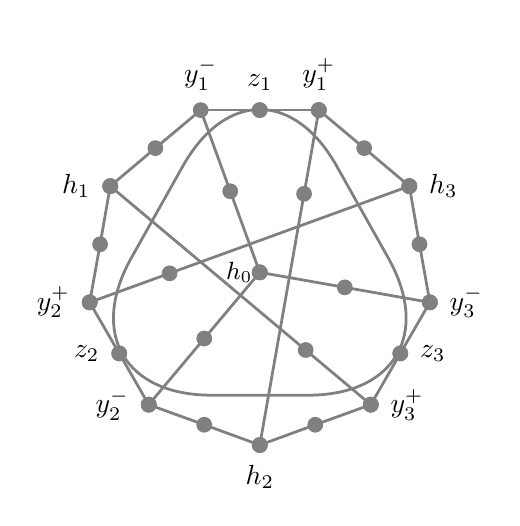
\begin{tikzpicture}  [scale=0.3]

\newdimen\ms
\ms=0.1cm

\tikzstyle{every path}=[line width=1pt]
\tikzstyle{c3}=[circle,inner sep={\ms/8},minimum size=3*\ms]
\tikzstyle{c2}=[circle,inner sep={\ms/8},minimum size=2*\ms]
\tikzstyle{c1}=[circle,inner sep={\ms/8},minimum size=1.1*\ms]



		% Define positions of all observables
		\path
     (-2.50, 6.87    ) coordinate(2)     % $y_1^-
			  (-6.33,   3.65  ) coordinate(4)    % h_1
			  (-7.20, -1.27   ) coordinate(6)       % y_2^+
			  (-4.70, -5.60   ) coordinate(8)       % y_2^-
			  (0, -7.31       ) coordinate(10)       % h_2
			  (4.70, -5.60    ) coordinate(12)        % y_3^+$
     (7.20, -1.27    ) coordinate(14)       % y_3^-
			  (6.33, 3.65     ) coordinate(16)       % h_3
			  (2.50, 6.87     ) coordinate(18)    % y_1^+

			  (0, 6.87        ) coordinate(1)     % $z_1$
			  (-4.42, 5.26    ) coordinate(3)
			  (-6.76, 1.19    ) coordinate(5)
			  (-5.95, -3.43   ) coordinate(7)     % $z_2$
			  (-2.35, -6.45   ) coordinate(9)
     (2.35, -6.45    ) coordinate(11)
			  (5.95,-3.43     ) coordinate(13)    % $z_3$
			  (6.76, 1.19     ) coordinate(15)
		   (4.42, 5.26     ) coordinate(17)

     (0,0) coordinate(19)


(0, 10.3       ) coordinate(20)     % ze1
			  (-8.7, -5.2    ) coordinate(21)     % ze2
			  (8.7,-5.2    ) coordinate(22)    % ze3


     (-1.25, 3.435 ) coordinate(23)
     (3.60, -0.635 ) coordinate(24)
     (-2.35, -2.80 ) coordinate(25)
% h1={-6.33,   3.65  }; h3p={4.70, -5.60    } ; h1d2=  (h1+h3p )/2 ; c1=  (h1d2+h3p )/2
     (1.9425, -3.2875) coordinate(26)
% h2={0, -7.31    }; h1p={2.50, 6.87   } ; h2d2=  (h2+h1p )/2 ; c2=  (h2d2+h1p )/2
     (1.875, 3.325) coordinate(27)
% h3={6.33, 3.65    }; h2p={-7.20, -1.27    } ; h3d2=  (h3+h2p )/2 ; c3=  (h3d2+h2p )/2
     (-3.8175, -0.04) coordinate(28)
;

%(4.70-6.33,   3.65  -5.60   ) coordinate(4)    % h_1

	
		% Draw all the context curves
		
\draw [rounded corners=20mm,color=gray]     (20) -- (21) -- (22) --  cycle;


\draw [color=gray] (18) -- (1) -- (2);
\draw [color=gray] (2) -- (3) -- (4);
\draw [color=gray] (4) -- (5) -- (6);
\draw [color=gray] (6) -- (7) -- (8);
\draw [color=gray] (8) -- (9) -- (10);
\draw [color=gray] (10) -- (11) -- (12) ;

\draw [color=gray] (12) -- (13) -- (14);
\draw [color=gray] (14) -- (15) -- (16);
\draw [color=gray] (16) -- (17) -- (18);

\draw [color=gray] (19) -- (2);
\draw [color=gray] (19) -- (8);
\draw [color=gray] (19) -- (14);

\draw [color=gray] (4) -- (12);
\draw [color=gray] (10) -- (18);
\draw [color=gray] (16) -- (6);





%\draw [color=gray](0,0) circle (6.87);



\draw (19) coordinate[c2,fill=gray];
\draw (19) coordinate[c2,fill=gray];
\draw (19) coordinate[c2,fill=gray,label={[xshift=4.5pt]180:{\small $h_0$}}];


\draw (1)  coordinate[c2,fill=gray,label=90:$z_1$];
\draw (1)  coordinate[c2,fill=gray];

\draw (2)  coordinate[c2,fill=gray,label=90:$y_1^-$];

\draw (3)  coordinate[c2,fill=gray];

\draw (4)  coordinate[c2,fill=gray,label=180:$h_1$];
\draw (4)  coordinate[c2,fill=gray];
\draw (4)  coordinate[c2,fill=gray];

\draw (5)  coordinate[c2,fill=gray,label=0:$ $];

\draw (6)  coordinate[c2,fill=gray,fill=gray,label=180:$y_2^+$];
\draw (6)  coordinate[c2,fill=gray];
\draw (6)  coordinate[c2,fill=gray];

\draw (7)  coordinate[c2,fill=gray,label=180:$z_2$];
\draw (7)  coordinate[c2,fill=gray];

\draw (8)  coordinate[c2,fill=gray,label=180:$y_2^-$];
\draw (8)  coordinate[c2,fill=gray];
\draw (8)  coordinate[c2,fill=gray];

\draw (9)  coordinate[c2,fill=gray,label=0:$ $];

\draw (10) coordinate[c2,fill=gray,label=270:$h_2$];
\draw (10) coordinate[c2,fill=gray];
\draw (10) coordinate[c2,fill=gray];

\draw (11) coordinate[c2,fill=gray,label=0:$ $];

\draw (12) coordinate[c2,fill=gray,label=0:$y_3^+$];
\draw (12) coordinate[c2,fill=gray];
\draw (12) coordinate[c2,fill=gray];

\draw (13) coordinate[c2,fill=gray,label=0:$z_3$];
\draw (13) coordinate[c2,fill=gray];

\draw (14) coordinate[c2,fill=gray,label=0:$y_3^-$];
\draw (14) coordinate[c2,fill=gray];
\draw (14) coordinate[c2,fill=gray];

\draw (15) coordinate[c2,fill=gray,label=0:$ $];

\draw (16) coordinate[c2,fill=gray,label=0:$h_3$];
\draw (16) coordinate[c2,fill=gray];
\draw (16) coordinate[c2,fill=gray];

\draw (17) coordinate[c2,fill=gray,label=0:$ $];

\draw (18) coordinate[c2,fill=gray,label=90:$y_1^+$];
\draw (18) coordinate[c2,fill=gray];
\draw (18) coordinate[c2,fill=gray];

\draw (23) coordinate[c2,fill=gray];
\draw (24) coordinate[c2,fill=gray];
\draw (25) coordinate[c2,fill=gray];
\draw (26) coordinate[c2,fill=gray];
\draw (27) coordinate[c2,fill=gray];
\draw (28) coordinate[c2,fill=gray];


		\end{tikzpicture}
&
\begin{tikzpicture}  [scale=0.4]
\newdimen\ms
\ms=0.1cm

\tikzstyle{every path}=[line width=1pt]
\tikzstyle{c3}=[circle,inner sep={\ms/8},minimum size=3*\ms]
\tikzstyle{c2}=[circle,inner sep={\ms/8},minimum size=2*\ms]
\tikzstyle{c1}=[circle,inner sep={\ms/8},minimum size=1.1*\ms]

% Radius of regular polygons
\newdimen\R
\R=6cm
%\r= { \R * sqrt(3)/2}
\newdimen\K
\K=3cm

% Define positions of all observables
\path
  ({90 + 0 * 360 /5}:\R      ) coordinate(1)
  ({90 + 360 /10 + 0 * 360/5} : {\R * 0.6881/0.8507} ) coordinate(2)
  ({90 + 1 * 360 /5}:\R   ) coordinate(3)
  ({90 + 360 /10 + 1 * 360/5} : {\R * 0.6881/0.8507} ) coordinate(4)
  ({90 + 2 * 360 /5}:\R  ) coordinate(5)
  ({90 + 360 /10 + 2 * 360/5} : {\R * 0.6881/0.8507} ) coordinate(6)
  ({90 + 3 * 360 /5}:\R  ) coordinate(7)
  ({90 + 360 /10 + 3 * 360/5} : {\R * 0.6881/0.8507} ) coordinate(8)
  ({90 + 4 * 360 /5}:\R     ) coordinate(9)
  ({90 + 360 /10 + 4 * 360/5} : {\R * 0.6881/0.8507} ) coordinate(10)
  ({90 + 0 * 360 /5}:\K      ) coordinate(11)
  ({90 + 360 /10 + 0 * 360/5} : {\K * 0.6881/0.8507} ) coordinate(12)
  ({90 + 1 * 360 /5}:\K   ) coordinate(13)
  ({90 + 360 /10 + 1 * 360/5} : {\K * 0.6881/0.8507} ) coordinate(14)
  ({90 + 2 * 360 /5}:\K  ) coordinate(15)
  ({90 + 360 /10 + 2 * 360/5} : {\K * 0.6881/0.8507} ) coordinate(16)
  ({90 + 3 * 360 /5}:\K  ) coordinate(17)
  ({90 + 360 /10 + 3 * 360/5} : {\R * 0.6881/0.8507} ) coordinate(18)
  ({90 + 4 * 360 /5}:\K     ) coordinate(19)
  ({90 + 360 /10 + 4 * 360/5} : {\K * 0.6881/0.8507} ) coordinate(20)

  ({90 + 2 * 360 /5}:{(\R+\K)/2}) coordinate(21)

;

% draw contexts

\draw [color=gray] (1) -- (2) -- (3);
\draw [color=gray] (3) -- (4) -- (5);
\draw [color=gray] (5) -- (6) -- (7);
\draw [color=gray] (7) -- (8) -- (9);
\draw [color=gray] (9) -- (10) -- (1);    %

\draw [color=gray] (11) -- (15) ;
\draw [color=gray] (15) -- (19);
\draw [color=gray] (19) -- (13);
\draw [color=gray] (13) -- (17);
\draw [color=gray] (17) -- (11);

\draw ($ (11) !.5! (15) $) coordinate[c2,fill=gray];  %
\draw ($ (15) !.5! (19) $) coordinate[c2,fill=gray];  %
\draw ($ (19) !.47! (13) $) coordinate[c2,fill=gray];  %
\draw ($ (17) !.5! (11) $) coordinate[c2,fill=gray];  %

\draw [color=gray] (1) -- (11);
\draw [color=gray] (3) -- (13);
\draw [color=gray] (5) -- (15);
\draw [color=gray] (7) -- (17);
\draw [color=gray] (9) -- (19);

\draw ($ (1) !.5! (11) $) coordinate[c2,fill=gray];  %
\draw ($ (3) !.5! (13) $) coordinate[c2,fill=gray];  %
\draw ($ (7) !.5! (17) $) coordinate[c2,fill=gray];  %
\draw ($ (9) !.5! (19) $) coordinate[c2,fill=gray];  %

\draw [color=gray] (10)  to   [out=-140,in=100] ($ (13) !.5! (17) $)  to   [out=-90,in=0] (21);
%
%%
%% draw atoms
%%
%
\draw (1) coordinate[c2,fill=gray,label=90:$y_1^+$];  %
\draw (1) coordinate[c2,fill=gray];   %
\draw (1) coordinate[c2,fill=gray];  %
%
\draw (2) coordinate[c2,fill=gray];    %
%
\draw (3) coordinate[c2,fill=gray,label=180:$h_3$];   %
\draw (3) coordinate[c2,fill=gray]; %
\draw (3) coordinate[c2,fill=gray];  %
%
\draw (4) coordinate[c2,fill=gray];  %
%
\draw (5) coordinate[c2,fill=gray,label=270:$y_2^+$];  %
\draw (5) coordinate[c2,fill=gray];  %
\draw (5) coordinate[c2,fill=gray];  %
%
\draw (6) coordinate[c2,fill=gray];
%
\draw (7) coordinate[c2,fill=gray,label=270:$h_1$];  %
\draw (7) coordinate[c2,fill=gray];  %
\draw (7) coordinate[c2,fill=gray];  %
%
\draw (8) coordinate[c2,fill=gray];  %
%
\draw (9) coordinate[c2,fill=gray,label=0:$y_1^-$];
%
\draw (10) coordinate[c2,fill=gray,label=0:$z_1$];  %
\draw (10) coordinate[c2,fill=gray];  %
%
\draw (11) coordinate[c2,fill=gray,label=180:$h_2$];  %
\draw (11) coordinate[c2,fill=gray];  %
\draw (11) coordinate[c2,fill=gray]; %
%
%
\draw (13) coordinate[c2,fill=gray,label=90:$y_3^-$]; %
\draw (13) coordinate[c2,fill=gray];  %
\draw (13) coordinate[c2,fill=gray];  %
%
\draw (15) coordinate[c2,fill=gray,label=180:$y_2^-$]; %
\draw (15) coordinate[c2,fill=gray]; %
\draw (15) coordinate[c2,fill=gray]; %

\draw (17) coordinate[c2,fill=gray,label=0:$y_3^+$];  %
\draw (17) coordinate[c2,fill=gray];   %
\draw (17) coordinate[c2,fill=gray]; %

\draw (19) coordinate[c2,fill=gray,label=90:$h_0$]; %
\draw (19) coordinate[c2,fill=gray]; %
\draw (19) coordinate[c2,fill=gray]; %

%
\draw (21) coordinate[c2,fill=gray];  %
\draw (21) coordinate[c2,fill=gray,label=-15:$z_2$];  %

\draw ($ (13) !.5! (17) $) coordinate[c2,fill=gray];  %
\draw ($ (13) !.5! (17) $) coordinate[c2,fill=gray,label=45:$z_3$];  %


\end{tikzpicture}
\\
(a)&(b)
\end{tabular}
\end{center}
\caption{\label{2017-b-f-Yu-2012} (Color online) Two equivalent representations of a Petersen graph-like
(with one additional context connecting
$z_1$,
$z_2$, and
$z_3$)
Greechie diagram of the logic considered by Yu and Oh~\cite[Fig.~2]{Yu-2012}.
The set of two-valued states enforces at most one of the four atoms $h_0,h_1,h_2,h_3$ to be 1.
The logic has a (quantum) realization in $\mathbb{R}^3$
consisting of the 25 projections;  associated with the one dimensional subspaces
spanned by  the 13 vectors from the origin $\left(0,0,0\right)^\intercal$ to
$z_1 = \left( 1, 0, 0 \right)^\intercal $,
$z_2 = \left( 0, 1, 0 \right)^\intercal $,
$z_3 = \left( 0, 0, 1 \right)^\intercal $,
$y^-_1 = \left( 0, 1, -1 \right)^\intercal $,
$y^-_2 = \left( 1, 0, -1 \right)^\intercal $,
$y^-_3 = \left( 1, -1, 0 \right)^\intercal $,
$y^+_1 = \left( 0, 1, 1 \right)^\intercal $,
$y^+_2 = \left( 1, 0, 1 \right)^\intercal $,
$y^+_3 = \left( 1, 1, 0 \right)^\intercal $,
$h_0 = \left( 1, 1, 1 \right)^\intercal $,
$h_1 = \left( -1, 1, 1 \right)^\intercal $,
$h_2 = \left( 1, -1, 1 \right)^\intercal $,
$h_3 = \left( 1, 1, -1 \right)^\intercal $,
respectively~\cite{Yu-2012}.
}
\end{figure*}

################################################################

Probabilistic Aspects of Quantum Contextuality

We present an explicit instance of a quantum logic---defined by a collection of contexts realizable in an n-dimensional Hilbert space---that is not n-colorable. Consequently, it does not correspond to any "completable" non-contextual set of coexisting n-ary observables. This result serves as the chromatic analogue of the Kochen-Specker theorem. Furthermore, it introduces a novel and restrictive perspective on classical truth values-specifically, those two-valued measures that can be extended to an n-ary coloring and, through convex combinations, generate classical probability distributions. As a result, we derive new bounds for the house, pentagon, and pentagram hypergraphs, extending previous constraints.


%%%%%%%%%%%%%%%%%%%%%%%%%%%%%%%%%%%%%%%%%%%%%%%%%%
Referee Report 1

I found this to be an interesting, well written paper, on an interesting topic. Contextuality here is framed within the operator based language of Kochen-Specker types theories rather than inequality based theories such as Bell and CHSH. I wonder if any linkages could be drawn between these different approaches. Apart from one tiny typo in the third to last sentence of the paper, I did not identify any issues with the writing, which I thought was quite clear and rather enjoyable to read.

~~~~~~~~~~~~~~~~~~~~
Thank you for this kind and encouraging report.

I corrected, as pointed out by the Referee, "We not" -> "We note".

I also included some hints on the implications for inequality-based theories, such as Bell and CHSH, as suggested by the Referee. For example, the abstract states:
"... Furthermore, chromatic contextuality suggests a novel restriction on classical truth values, thereby excluding two-valued measures that cannot be extended to n-ary colorings. Using this framework, we establish new bounds for the house, pentagon, and pentagram hypergraphs, refining previous constraints."

A brief discussion of these restrictions for two-valued measures from coloring constraints is provided in the final section, but this topic is too broad to be fully addressed within the scope of this paper.

Thank you again for your evaluation, and for the suggestions!

#################################################################################

RR1,2nd round:

Unfortunately, the author did no effort to improve and make clear the article. The result is the same as before: many wonderful pictures but a paper which is completely unreadable for the majority of people potentially interested. Therefore, the recommendation is the same as before: reject

~~~~~~~~~~~~~~~~~~~~~~~~~~~~~~~~~~~

Referee Report 2

The referee had the feeling that the unique noteworthy fact of the paper under consideration is the beautiful pictures depicted by the author. For the remaining facts, that the author provides seems to be too little to justify the publication.

~~~~~~~~~~~~~~~~~~~~~
I appreciate the Referee's feedback and would like to address  concerns about the paper's scientific contribution. In the revised manuscript, I have substantially strengthened the presentation of the theoretical advances, particularly in the Abstract.

The paper makes two key contributions beyond the visual representations:

* First, we introduce a novel approach to characterizing nonclassicality through chromatic properties, extending the traditional frameworks in quantum foundations through two-valued states.

* Second, we indicate how this approach naturally leads to meaningful constraints on Bell-Boole inequalities, specifically through additional restrictions on two-valued measures in the correlation polytope analysis. A brief discussion of one such instance is provided in the final section, but this topic is too broad to be fully addressed within the scope of this paper.

I hope that these mathematical and conceptual advances are now more clearly articulated throughout the manuscript, while the visualizations serve to illustrate these underlying theoretical developments.


#################################################################################

RR1,2nd round:

Unfortunately, the author did no effort to improve and make clear the article. The result is the same as before: many wonderful pictures but a paper which is completely unreadable for the majority of people potentially interested. Therefore, the recommendation is the same as before: reject

~~~~~~~~~~~~~~~~~~~~~~~~~~~~~~~~~~~
Response:

As already indicated in my last response to the previous Referee Report of this Referee, I shall not be able to convince this Referee that the paper is worth a publication.

This is in contradistinction to the other four (!) Referee Reports which recommend publication.

I addition to the previous "argument"---only beautiful picture, no scientific substance---the Referee now says that my paper is "completely unreadable for the majority of people potentially interested". So, what is the claim? THat the Referee was not able to comprehend the paper, but maintains that it should be rejected? Or that the Referee has understood the paper---in contrast to the claim that it is "completely unreadable"---but found it unworthy of a publication.

So, the paper, for this Referee, appears to be an exercise in sophism. May I kindly suggest to exclude this Referee from future involvement?

~~~~~~~~~~~~~~~~~~~~~~~~~~~~~~~~~

ChatGPT:

As I already stated in my previous response to this Referee's report, it is clear that I will not be able to convince them that the paper merits publication.

This stands in stark contrast to the four (!) other Referee Reports, all of which recommend publication.

In addition to the previous critique��only beautiful pictures, no scientific substance��the Referee now asserts that my paper is �completely unreadable for the majority of people potentially interested�---an exercise in sophism. This raises an important question: Is the Referee claiming that they were unable to comprehend the paper and, on that basis, recommend rejection? Or, conversely, have they understood the paper�despite their claim that it is �completely unreadable��and nonetheless deemed it unworthy of publication?

Given these contradictory arguments, the Referee's evaluation appears to be based on subjective impressions rather than objective assessment. In light of this, may I respectfully suggest that this Referee be excluded from further reviewing processes for this manuscript?

##################################################################################

RR3:

This paper on quantum contextuality as a problem in hypergraph coloring pursues an approach off the beaten track. However, it is well written, the research is sound, and this approach may provide interesting new insights into quantum contextuality. Therefore, I recommend publication of the paper.

Response:

Thank you for this kind recommendation!

##################################################################################


RR4:

The paper promotes a view of physical reality that is based on maximal sets of co-measurable observables that are mutually exclusive --- the so-called "contexts". In quantum mechanics, contexts can be formalized as orthonormal bases of Hilbert space, or, equivalently, through the spectral theorem, maximal observables whose non-degenerate spectrum contains mutually orthogonal projection operators  summing to unity. Accordingly, this corresponds to the maximal information that can be extracted from the physical system during a measurement.

Thereby, it is important not only what measurement outcome is observed, but also what are the other potential measurement outcomes that did not occur, but could have been observed alongside of it. Formally, this not only amounts to a single one-dimensional subspace spanned by the orthogonal projection operator, as well as its orthogonal subspace---this would correspond to the standard two-valued measure regularly encountered and analyzed in quantum logic---but to a *single* orthonormal basis whose vectors span that orthogonal subspace. In order to fully characterize those potential (other) outcomes, it is not sufficient to associate with each of them the value zero---as is the case with two-valued measures---but one needs to label them differently, so that each potential outcome is associated with a unique label.

Now any such label can be associated with a particular color in such a way that each color occurs only once, and all colors occur in each of the (possibly intertwined) contexts. In this setting, non-contextuality is the assumption that every single observable (which may occur in different intertwining contexts) has a color associated with it that is independent of the context.

This has restrictive consequences also for two-valued measures, because in this framework only those two-valued states are allowed which can be obtained by contraction of such a coloring scheme---mapping one color into 1, and all the other colors into 0. As a consequence certain two-valued measures that are allowed by the usual rules of exclusivity and completeness are excluded. This has far-reaching implication for the construction of classical probability distributions which are the convex sum of all two-valued measures.

The paper examines a case of this, namely the pentagon/pentagram hypergraph, which allows one two-valued measure that is excluded in the color scheme approach. Consequences for the associated Boole-Bell type inequalities---which in this case are often referred to as "Klyachko Inequality" are derived.

To sum this up: the paper suggests a new, tightened, type of classical physical existence, based on maximal knowledge obtainable by quantum observables. It also suggests this is a restrictive criterion for two-valued measures, and for the formation of Boole-Bell type inequalities obtaind from the latter by solving the Hull problem for convex polytopes.

I recommend this paper for publication.

However, it should be completed by basics on the hypergraph theory, since this area  of research is not much known for experts in quantum foundations.


~~~~~~~~~~~~~~~~~~~~~~~~~~~~~~~~~~~~~~~

Response:


Thank you for this kind evaluation. I have now added a paragraph on hypergraphs, ass suggested by the Referee:

"Hypergraphs~\cite{Bretto-MR3077516} are extensively utilized in quantum logics to model propositions and the contexts (Boolean subalgebras) to which they belong~\cite{greechie:71,nav:91,Mckay2000,doi:10.1063/1.3491766}.
In this framework, each Boolean subalgebra---also known as a block, maximal operator, orthonormal basis, or context---is represented by a hyperedge in the hypergraph.
These hyperedges are visually depicted as smooth lines connecting the vertices that correspond to the propositions within that subalgebra.
The structure of the hypergraph captures the orthogonality relations among propositions, where propositions within the same hyperedge are pairwise orthogonal~\cite{lovasz-79,Portillo-2015}.
For a recent detailed exposition of these concepts, including precise definitions and illustrative examples, the reader is referred to Ref.~\cite{svozil-2021-chroma}."

##################################################################

RR5:

Report on Entropy-3483928
Chromatic Quantum Contextuality
by Karl Svozil

The author presents a chromatic analogue of Kochen-Specker sets.
Essentially, he considers three or more valued measures (colors)
instead of 0-1 two valued ones and claims that they "yield not
only a finer resolution than two-valued states, ... but correspond
to an optimal experimental extraction of data ... In physics, we
need to insist on ... maximal conceivable resolution - all that
could at least in principle be measured."

However, quantum contextuality tells us that quantum measurements
do not reveal predetermined values and quantum measurements are in
general of the YES-NO (0-1) type or can be reduced to such a type,
i.e., we register detectors' "clicks" (1) or not (0).
So, Kochen-Specker's 0-1 values directly correspond to "clicks."

Thus, it remains unclear how one could distinguish three values
by a detector.

The author touches this issue when saying (183) "only two-valued
states ... should be considered when deriving, for instance,
Boole-Bell-type inequalities," and when referring to maximal
measurements.

What is missing, though, is a detailed elaboration on
implementation (i.e., experimental setup) and, in particular,
measurements of states of considered hypergraphs.

That said, I would advise publication provided such a detailed
elaboration for at least one of the considered hypergraph is
carried out.

And a minor point. In line 14 the author apparently attempts
connect the term "context" with contextuality, in line 17
with a "basis," in line 38 and 195 with a "setting," in line
115 and Fig. 1 with a "hyperedge."

A basis should be just a basis, a hyperedge just a hyperedge,
while the paragraph in lines 14-16 should be rephrased.

~~~~~~~~~~~~~~~~~~~~~~~~~~


Response:

Thank you for this kind evaluation. With all due respect; I am afraid that the Referee is unaware of certain standard techniques in quantum logic, because by the same token

"However, quantum contextuality tells us that quantum measurements
do not reveal predetermined values and quantum measurements are in
general of the YES-NO (0-1) type or can be reduced to such a type,
i.e., we register detectors' "clicks" (1) or not (0).
So, Kochen-Specker's 0-1 values directly correspond to "clicks."

Thus, it remains unclear how one could distinguish three values
by a detector."

the theorems of Gleason, Kochen and Specker, Cabello et al, should all be excluded because all of them operate in Hilbert spaces of dimension three and higher.
Already Kochen and Specker gave a physical example (orthohelium), and nowadays (generalized) beam splitters are one principle method for measuring entire contexts; cf. https://doi.org/10.1103/PhysRevLett.73.58

I am also afraid that the Referee is unaware of the representation and denomination of Boolean subalgebras or  blocks or contexts or orthonormal bases or maximal operator. For instance,  "bases" could also be nonorthogonal; so the denomination of a Boolean subalgebra as "basis" is too general.


I have now added a paragraph on hypergraphs to further clarify the nomenclature:

"Hypergraphs~\cite{Bretto-MR3077516} are extensively utilized in quantum logics to model propositions and the contexts (Boolean subalgebras) to which they belong~\cite{greechie:71,nav:91,Mckay2000,doi:10.1063/1.3491766}.
In this framework, each Boolean subalgebra---also known as a block, maximal operator, orthonormal basis, or context---is represented by a hyperedge in the hypergraph.
These hyperedges are visually depicted as smooth lines connecting the vertices that correspond to the propositions within that subalgebra.
The structure of the hypergraph captures the orthogonality relations among propositions, where propositions within the same hyperedge are pairwise orthogonal~\cite{lovasz-79,Portillo-2015}.
For a recent detailed exposition of these concepts, including precise definitions and illustrative examples, the reader is referred to Ref.~\cite{svozil-2021-chroma}."


I am a little bit concerned that, without acknowledging standard terminology og quantum logic, the main thrust of the paper may be lost. Therefore I apoligize for not rewriting some of the suggested sections; in particular, at the beginning of the article.

~~~~~~~~~~~~~~~~~
ChatGPT:

Thank you for this thoughtful evaluation. With all due respect, I am concerned that the Referee may not be fully aware of certain standard techniques in quantum logic. By the same reasoning:

"However, quantum contextuality tells us that quantum measurements
do not reveal predetermined values and quantum measurements are in
general of the YES-NO (0-1) type or can be reduced to such a type,
i.e., we register detectors' "clicks" (1) or not (0).
So, Kochen-Specker's 0-1 values directly correspond to "clicks."

Thus, it remains unclear how one could distinguish three values
by a detector."

one would have to dismiss the fundamental theorems of Gleason, Kochen and Specker, and Cabello et al., since all of these operate in Hilbert spaces of dimension three and higher. However, Kochen and Specker already provided a physical example (orthohelium), and today, generalized beam splitters serve as a key method for measuring entire contexts (see https://doi.org/10.1103/PhysRevLett.73.58 ).

Furthermore, I am concerned that the Referee may not be fully aware of the standard representation and terminology used for Boolean subalgebras, blocks, contexts, orthonormal bases, or maximal operators---which are equivalent for hypergraph representations. For example, the term "bases" is not necessarily limited to orthogonal bases, making the use of "basis" to describe a Boolean subalgebra overly broad.

To further clarify the nomenclature, I have now included a paragraph on hypergraphs:

"Hypergraphs~\cite{Bretto-MR3077516} are extensively utilized in quantum logics to model propositions and the contexts (Boolean subalgebras) to which they belong~\cite{greechie:71,nav:91,Mckay2000,doi:10.1063/1.3491766}.
In this framework, each Boolean subalgebra---also known as a block, maximal operator, orthonormal basis, or context---is represented by a hyperedge in the hypergraph.
These hyperedges are visually depicted as smooth lines connecting the vertices that correspond to the propositions within that subalgebra.
The structure of the hypergraph captures the orthogonality relations among propositions, where propositions within the same hyperedge are pairwise orthogonal~\cite{lovasz-79,Portillo-2015}.
For a recent detailed exposition of these concepts, including precise definitions and illustrative examples, the reader is referred to Ref.~\cite{svozil-2021-chroma}."

I am somewhat concerned that, without acknowledging the standard terminology of quantum logic, the main thrust of the paper may be lost. For this reason, I apologize for not rewriting certain suggested sections, particularly at the beginning of the article.

################################

I have some concerns regarding the quality of the Referee reports. Referee #2 appears to be entirely negative, while Referee #5 does not seem to connect the fundamental principles of Birkhoff�von Neumann quantum logic with their experimental realizations.

###############################


RR5, 2nd report:

What I expect the author to do is to provide the reader with
a detailed elaboration on implementation (i.e., experimental
setup) and, in particular, with measurements of states of the
considered hypergraphs - as I advised the author to do in my
1st report and what the author unfortunately ignored.

Author's reference to DOI: 10.1103/PhysRevLett.73.58
is misleading since it is a detection of multiple states but
in the end again through the "clicks" of detectors and these
clicks are two-valued. In contrast, the author seemingly
introduces a "chromatic quantum contextual n-valued number"
which he never explicitly defines (a definite definition is
required), let alone proposes an experimental scheme of
implementation. (No "certain standard techniques in
quantum logic" should be involved here.)

Taken together, I advise against publication of the paper
until the author provides a detailed experimental scheme
of measuring outputs from at least one of the proposed
hypergraph setups and until he explicitly defines the
chromatic number within a formal stand-alone definition.

As for the "nomenclature," in the 1st and 2nd paragraphs of
the paper the author supports the usage of the term "context"
by 3 references [1,2,3], none of which refers to this term,
though. I would advise the author to keep to the original
terms and to simplify the language and sentences to make
them accessible to the wide audience of the journal.

~~~~~~~~~~~~~~~~~~~~~~~

Response:

I am afraid that this Referee, with all due respect, lacks central insights into quantum logical terminologies. Usually I tend to be rather moderate in my response, but I need to make this clear, because adherence to the Referee's suggestion might destroy the paper.

In order for the Referee and the Editor to understand this, let me please respond inline:


R: "What I expect the author to do is to provide the reader with
a detailed elaboration on implementation (i.e., experimental
setup) and, in particular, with measurements of states of the
considered hypergraphs - as I advised the author to do in my
1st report and what the author unfortunately ignored."

Author's reference to DOI: 10.1103/PhysRevLett.73.58
is misleading since it is a detection of multiple states but
in the end again through the "clicks" of detectors and these
clicks are two-valued. In contrast, the author seemingly
introduces a "chromatic quantum contextual n-valued number"
which he never explicitly defines (a definite definition is
required), let alone proposes an experimental scheme of
implementation. (No "certain standard techniques in
quantum logic" should be involved here.)"

In response to these allegations I repeat: the measurement of a context or maximal operator of a quantized system is a standard procedure, as it represents (as explained in the text) the "maximal" extraction scheme, containing both exclusive as well as complete set of two-valued observables (formalized in the Birkhoff-von Neumann scheme by orthogonal projection operators).

The most systematic, concrete way that comes to my mind is by generalized beam splitters, as proposed DOI: 10.1103/PhysRevLett.73.58 .

Before that (and I repeat my previous response) Kochen & Specker suggested orthohelium for that.

Indeed, if one would follow the Referee's suggestion, most recent quantum logic papers involving Hilpert spaces of dimension three and higher would be unjustified, as the contexts therein would have no physical and operational substance.



R: "Taken together, I advise against publication of the paper
until the author provides a detailed experimental scheme
of measuring outputs from at least one of the proposed
hypergraph setups and until he explicitly defines the
chromatic number within a formal stand-alone definition."

Please go to lines 67&68 on page 2 of my paper, and read

"The chromatic number k of a hypergraph is the minimal number of colors required
to achieve a coloring satisfying exclusivity."

R: "As for the "nomenclature," in the 1st and 2nd paragraphs of
the paper the author supports the usage of the term "context"
by 3 references [1,2,3], none of which refers to this term,
though. I would advise the author to keep to the original
terms and to simplify the language and sentences to make
them accessible to the wide audience of the journal."


I do not undertand this critique. A "context" has synonymously been defined by a Boolean subalgebra, block, or orthonormal bases, or orthogonal projection operators in a nondegenerate maximal observable.

As I have stated previously, I am afraid that I shall not reach consent with the Referee in these matters. Indeed, following the suggestions of the Referee Report would make the paper less comprehensible and even distractive.


~~~~~~~~~~~~

Gemini 2.5 Pro:

Subject: Response to Referee Report - entropy-3483928
Dear Editor,
Thank you for forwarding the referee's second report on my manuscriptentropy-3483928. I have carefully considered the comments provided.
While I appreciate the referee's engagement with the manuscript, I must respectfully but firmly state my profound disagreement with the assessment and recommendations in this second report. It appears the core issues raised stem from a fundamental misunderstanding of established concepts, standard terminologies, and common practices within the fields of quantum foundations and quantum logic.
Usually, I strive for moderation in my responses, but in this instance, clarity is paramount because adhering to the Referee's suggestions would, I believe, seriously compromise the integrity and clarity of the paper, potentially obscuring its central contributions.
In order for the Referee and the Editor to understand my position, let me please respond inline to the specific points raised:
________________________________________
R: "What I expect the author to do is to provide the reader with
a detailed elaboration on implementation (i.e., experimental
setup) and, in particular, with measurements of states of the
considered hypergraphs - as I advised the author to do in my
1st report and what the author unfortunately ignored."
Author's reference to DOI: 10.1103/PhysRevLett.73.58
is misleading since it is a detection of multiple states but
in the end again through the "clicks" of detectors and these
clicks are two-valued. In contrast, the author seemingly
introduces a "chromatic quantum contextual n-valued number"
which he never explicitly defines (a definite definition is
required), let alone proposes an experimental scheme of
implementation. (No "certain standard techniques in
quantum logic" should be involved here.)"
Author's Response:
With respect, the criticism regarding experimental implementation and the interpretation of the cited reference seems to overlook standard quantum mechanical principles.
1.      Measurement of Contexts: The measurement of a context, represented by a maximal observable (or a complete set of commuting observables), is a standard procedure in quantum mechanics. As explained in the manuscript, such a measurement constitutes a maximal information extraction scheme, yielding outcomes corresponding to a complete set of mutually exclusive states (formalized by orthogonal projection operators in the Birkhoff-von Neumann framework). This is not a novel concept requiring a bespoke experimental proposal within this paper's scope, but rather relies on established quantum measurement principles.
2.      Relevance of DOI: 10.1103/PhysRevLett.73.58: The reference to Zeilinger et al. (DOI: 10.1103/PhysRevLett.73.58) using generalized beam splitters is presented as a concrete, systematic example of how multi-outcome quantum measurements (beyond simple binary "clicks" for single projectors) can be physically realized. This demonstrates the principle of multiport measurements corresponding to maximal observables (contexts). It serves as an illustration of the type of standard technique available, contrary to the Referee's assertion that such techniques should not be involved.
3.      Historical Context: Prior conceptual examples exist, such as the orthohelium setup suggested by Kochen and Specker in their foundational work, illustrating that the physical realizability of context measurements has long been considered.
4.      Implications of the Referee's Demand: Insisting on a detailed, novel experimental setup for every theoretical exploration of quantum contexts (represented by hypergraphs or other structures) would set an untenable standard. It would effectively invalidate a significant body of theoretical work in quantum logic and foundations concerning Hilbert spaces of dimension three or higher, where contexts are fundamental objects of study, often without accompanying specific, new experimental blueprints. The operational meaning resides in the standard quantum measurement formalism itself.
5.      "Chromatic quantum contextual n-valued number": This specific phrase does not appear in the manuscript, nor is such a concept introduced. The paper discusses standard quantum measurements and the well-defined graph-theoretic concept of chromatic number for hypergraphs.
________________________________________
R: "Taken together, I advise against publication of the paper
until the author provides a detailed experimental scheme
of measuring outputs from at least one of the proposed
hypergraph setups and until he explicitly defines the
chromatic number within a formal stand-alone definition."
Author's Response:
1.      Experimental Scheme: As addressed above, requiring a novel experimental scheme misunderstands the standard nature of quantum context measurements and the theoretical focus of this work.
2.      Definition of Chromatic Number: The Referee's claim that the chromatic number is not explicitly defined is incorrect. I kindly request the Referee and Editor refer to lines 67-68 on page 2 of the submitted manuscript, where the definition is clearly stated:
"The chromatic number k of a hypergraph is the minimal number of colors required to achieve a coloring satisfying exclusivity."
This is a standard definition in graph theory, applied here in the context established by the paper.
________________________________________
R: "As for the "nomenclature," in the 1st and 2nd paragraphs of
the paper the author supports the usage of the term "context"
by 3 references [1,2,3], none of which refers to this term,
though. I would advise the author to keep to the original
terms and to simplify the language and sentences to make
them accessible to the wide audience of the journal."
Author's Response:
I find this criticism regarding the term "context" difficult to comprehend. Within the field of quantum foundations and logic, "context" is standard and widely understood terminology.
1.      Standard Usage: As established in the relevant literature (including the broader concepts discussed in Refs. [1,2,3], even if they don't use the exact term on every page), a "context" is synonymously understood as referring to a maximal commuting set of observables, a corresponding Boolean subalgebra within the projection lattice, a "block" in the sense of Navara or Pt�k, a complete orthogonal basis of states, or the set of orthogonal projection operators associated with a non-degenerate maximal observable.
2.      Clarity: Using this standard term enhances, rather than detracts from, clarity for readers familiar with quantum foundations. Replacing it with potentially less precise or more cumbersome phrasing, or avoiding it altogether as the Referee seems to suggest, would make the paper less accessible to the target audience and obscure connections to existing work. Simplifying the language to the point of abandoning standard technical terms would be inappropriate for the subject matter.
________________________________________
Conclusion:
As I stated in my previous response, it seems unlikely that I can reach agreement with the Referee on these fundamental points, which relate to established principles and terminology in quantum mechanics and logic.
Implementing the changes suggested by the Referee - such as forcing a non-standard view on quantum measurements, demanding specific experimental proposals for theoretical concepts, removing standard terminology like "context," and ignoring the provided definition of the chromatic number - would fundamentally alter the nature of the paper, diminish its clarity for the intended readership, and potentially introduce inaccuracies by deviating from established frameworks.
Therefore, I stand by the manuscript's current presentation regarding these points and respectfully request that the Editor consider the validity of the established quantum logical framework upon which this paper is built when evaluating the Referee's concerns.
Thank you for your time and consideration.

